\chapter{Muon Momentum Correction and Calibration} \label{chp:muon_corr}

This analysis aims to find a sharp signal peak on top of a smooth background in the \mmm distribution.
It is of crucial importance to correct any mismeasurement in the muon momentum scale 
and to remove any momentum dependence on variables like $\eta$ and $\phi$ of muons.
It is also crucial to minimize the momentum and resolution differences between data and simulation, 
so that there is no significant bias in the signal modeling.

Three sets of corrections are applied in this analysis: 
the \RochCorr~\cite{Bodek:2012id}, the recovery of the final-state radiation (FSR) photons, and the \GeoFit.
The \RochCorr is a centrally provided correction (by CMS), which corrects 
the biases in the muon momentum resulted from the mismodeling of detector alignment and magnetic field. 
A brief description of the \RochCorr is given in Section~\ref{sec:Roch_corr}, 
while the technical details can be found in the Ref.~\cite{Bodek:2012id}.
The \FSR is a common practice in many CMS analyses, which corrects the muon energy loss via FSR.
The recovery scheme in this analysis is optimized specifically for the \hmm decay, which is described in Section~\ref{sec:fsr} and in more detail in Ref.~\cite{oliverthesis}.
The \GeoFit is developed by the author in the context of the \hmm analysis and approved by the CMS collaboration.
It uses information of muon vertexing to correct the biases in muon momentum of the reconstructed muon tracks.
The development of the \GeoFit is described in details in Section~\ref{sec:GeoFit}.
The effects of the three corrections are orthogonal.
In practice, the \RochCorr is applied to all muons, then each muon is surveyed for FSR photons.
If an FSR photon is found associated to the muon, the \FSR is applied, 
if not, the \GeoFit is applied.\footnote{The performance of \GeoFit on muons with FSR is not validated and maybe suboptimal. 
Furthermore, as FSR muons are a small fraction, the difference whether to apply \GeoFit to them is negligible.}

These three corrections are applied to both data and simulation.
The performance of the corrections is examined with the study on the \zmm peak,
which is listed in details in Section~\ref{sec:muon_cal}.
These corrections fix all the known biases in muon measurement, 
and ensure a per-mille-level agreement between data and simulation. 

\section{Rochester Correction} \label{sec:Roch_corr}

In reality, the CMS detector can have various imperfections, 
such as the misalignment of the detector components, and the uncertainties in the magnetic field.
Sometimes these imperfections are not correctly emulated in reconstruction softwares, 
and as a result, the reconstructed muons can be inaccurate.
These inaccuracies are reflected as the dependences of the muon momentum on its \eta, \phi ~coordinates, and its charge.

On the other hand, in the simulation of CMS events, none of the imperfections are assumed,
which leads to slightly different detector responses from those in data, and in turn over-optimistic modelings in the muon measurement. 
Therefore the correction for simulation and for data have to be different.
The generated muon information, smeared with some functional forms to match the experimental resolution, 
is used as the reference for both data and simulation. 

The well-understood \zmm events are used to develop the \RochCorr. 
The idea of the correction is briefly summarized as follows:
\begin{itemize}
  \item For data, reconstructed simulation (reco-sim), and the reference simulation (ref-sim), 
        muons are divided into different \eta ~and \phi ~bins, separately for $\mu^{+}$ and $\mu^{-}$.
        In each bin, the $1/\pt$ distributions of data and reco-sim are corrected so that the mean value of the distribution becomes the same as that in the ref-sim.
  \item The $1/\pt$ distribution in reco-sim is usually narrower than that in data. 
        A smearing is applied to the reco-sim $1/\pt$ distribution so that it matches the resolution in data.
  \item After the steps above, the \mmm in each bin may still be off from the expected distribution by some small amounts.
        The ratio between this offset and the nominal \PZ mass is applied to the muon \pt as a correction factor iteratively, until the offset is minimized.
\end{itemize}
The \RochCorr removes the dependences of \mmm on muon \eta,~ \phi,~ and charge, 
as well as the \mmm resolution differences between data and the simulation.
Details of the performance of the \RochCorr can be found in Section~\ref{sec:muon_cal}.


\section{FSR Recovery} \label{sec:fsr}

In CMS, muons produced in $pp$ collisions may radiate photons and lose energy, which is referred to as the final-state radiation (FSR).
The radiation may carry substantial energy and lead to an underestimation of the original muon momentum.
This leads to two effects in this analysis:
a loss of event acceptance, and a smearing of the \mmm resolution.
This can be mitigated by identifying some of the FSR photons adding their energy back to the muon energy, called the \FSR.

The selection for the FSR photons is modified on top of the strategy developed in the CMS $\PH \to \PZ\PZ$ analyses~\cite{Sirunyan:2017exp, Sirunyan:2018qlb}.
The selection criteria is summarized as follows:
\begin{itemize}
  \item Photons with transverse energy $E^{\gamma}_{T} > $ 2 \GeV and $|\eta|<1.4$, $1.6<|\eta|<2.4$ are considered as FSR candidates.
  \item The photon is required to be within the cone of $\Delta{}R<0.5$ around its closest muon that satisfies $\pt >$ 20 \GeV and $|\eta| < 2.4$.
  \item The photon is not identified as a bremsstrahlung photon associated with a reconstructed electron.
  \item The PF isolation of the photon in a cone of $\Delta{}R < 0.3$ should be less than 1.8, i.e. $\sum_{i}\pt^{i}(\Delta{}R(\gamma, i)<0.3)/\pt(\gamma) < 1.8$, 
        where $i$ iterates the PF objects around the photon other than the candidate muon.
  \item The separation between the photon and the muon satisfies $\Delta{}R(\mu, \gamma)/\pt^{2}(\gamma) < 0.012$.
  \item In order to suppress energetic photons from the $\PH \to \PZ\gamma \to \mu\mu\gamma$ process,
        the \pt ratio between the photon and the muon is required to be less than 0.4, i.e. $\pt(\gamma)/\pt(\mu) < 0.4$.
  \item If multiple FSR photons are associated to the same muon, only the photon with the smallest $\Delta{}R(\mu, \gamma)/\pt^{2}(\gamma)$ is taken.
\end{itemize}

With this set of selection, about 3\% of signal events are tagged with FSR photons.
The selection is also very effective in reducing the $\PH \to \PZ\gamma$ events,
whose final yield is about 0.1\% of the overall \hmm signal and can be neglected.
The momentum of the FSR photons are added to the muon momentum, 
while the photons themselves are removed from the calculation of the muon isolation.
The \FSR significantly improves the \mmm reconstruction in the FSR tagged events, as shown in the left plot of Figure~\ref{fig:fsr_sig}.
The overall effect on the inclusive signal, as shown in the right plot of Figure~\ref{fig:fsr_sig}, 
is a 3\% improvement on the \mmm resolution and a 1.7\% increase in the total signal yield. 
The \FSR is applied in all categories of the \hmm analysis and resulting improvement on the combined significance is about 3\%.
The performance of \FSR is also validated with the \zmm events, shown in Figure~\ref{fig:fsr_val},
where a good agreement is kept between simulation and data with or without the \FSR. 
The \FSR is expected to perform the same way on data as on simulation, 
and no bias is introduced by the application of the \FSR. 

\begin{figure*}[!htb]
      \centering
%      \captionsetup{justification=justified}
      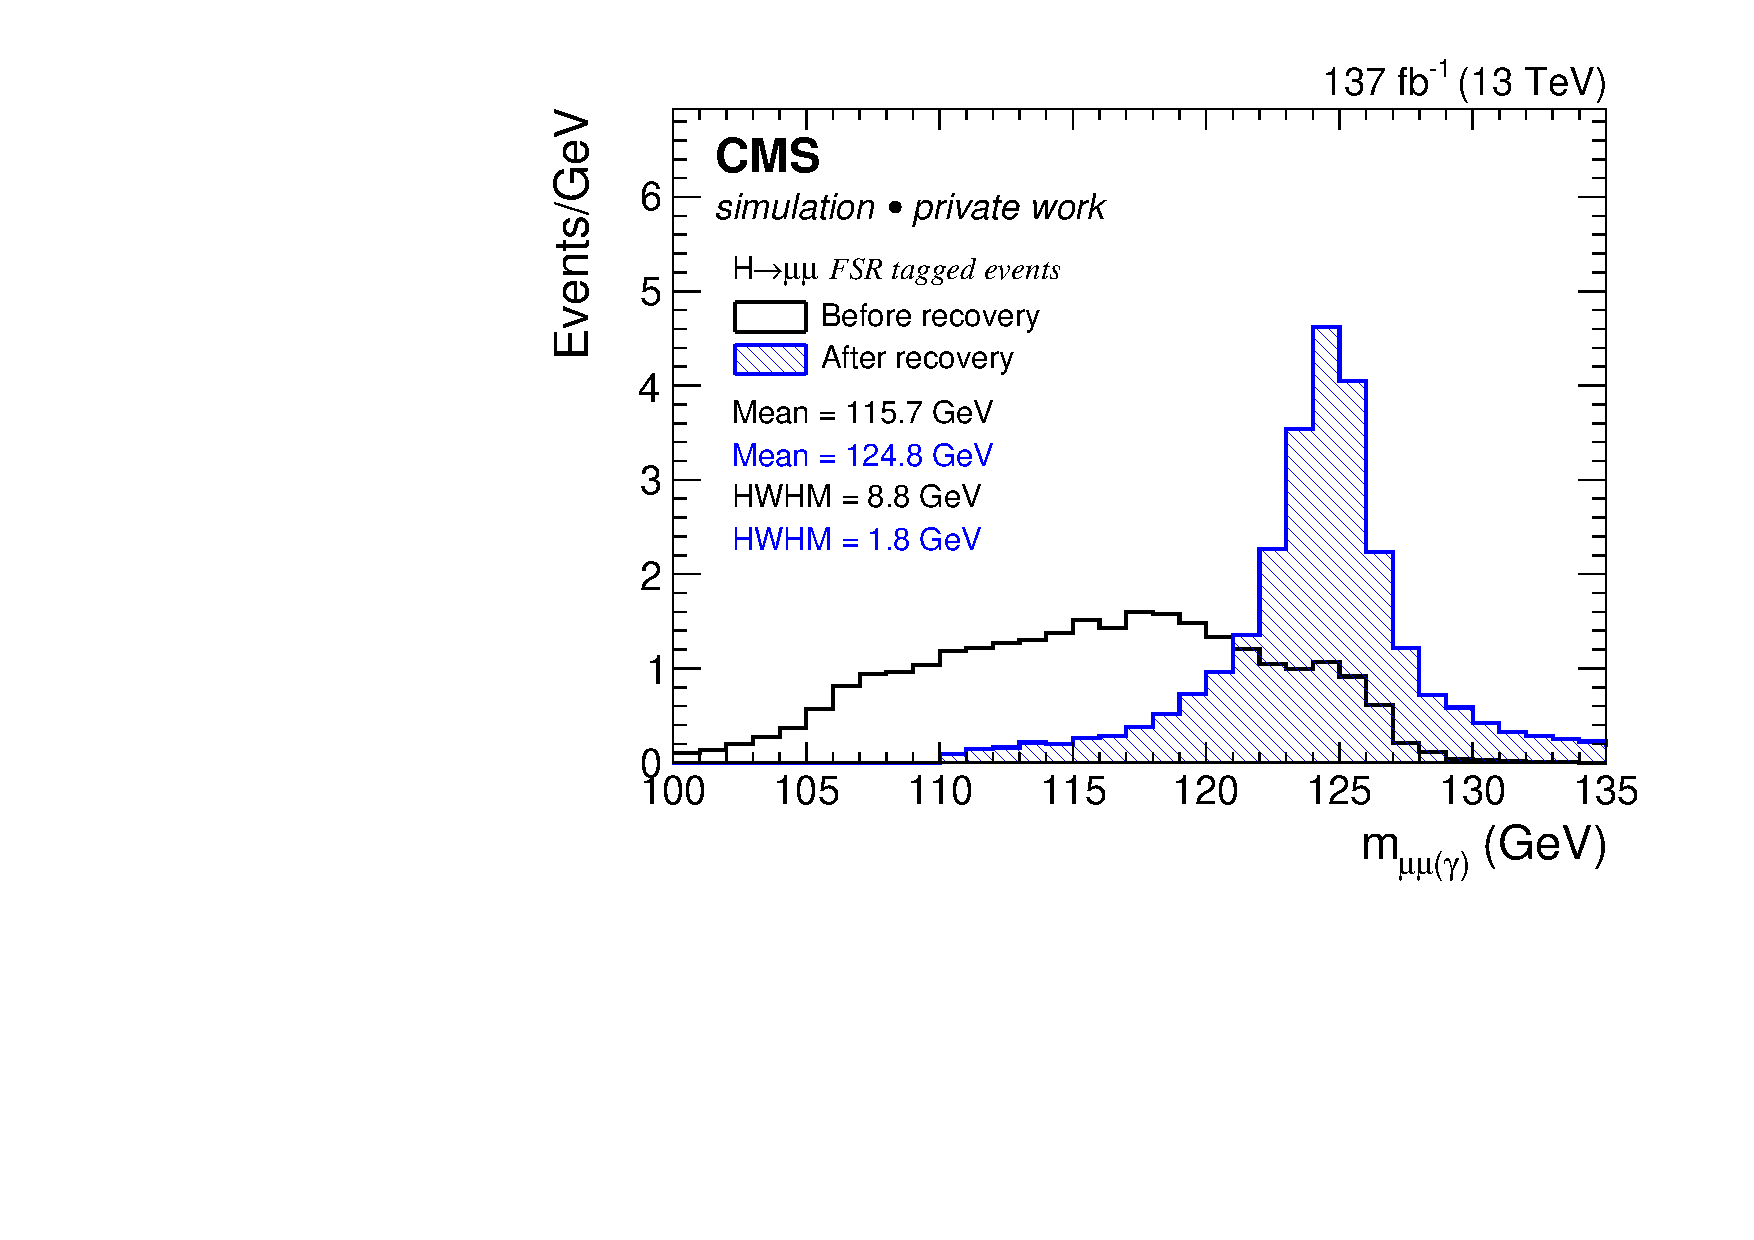
\includegraphics[width=0.45\textwidth]{pics/muon_corr/FSR/FSRrecovery_FSRtagged.pdf}
      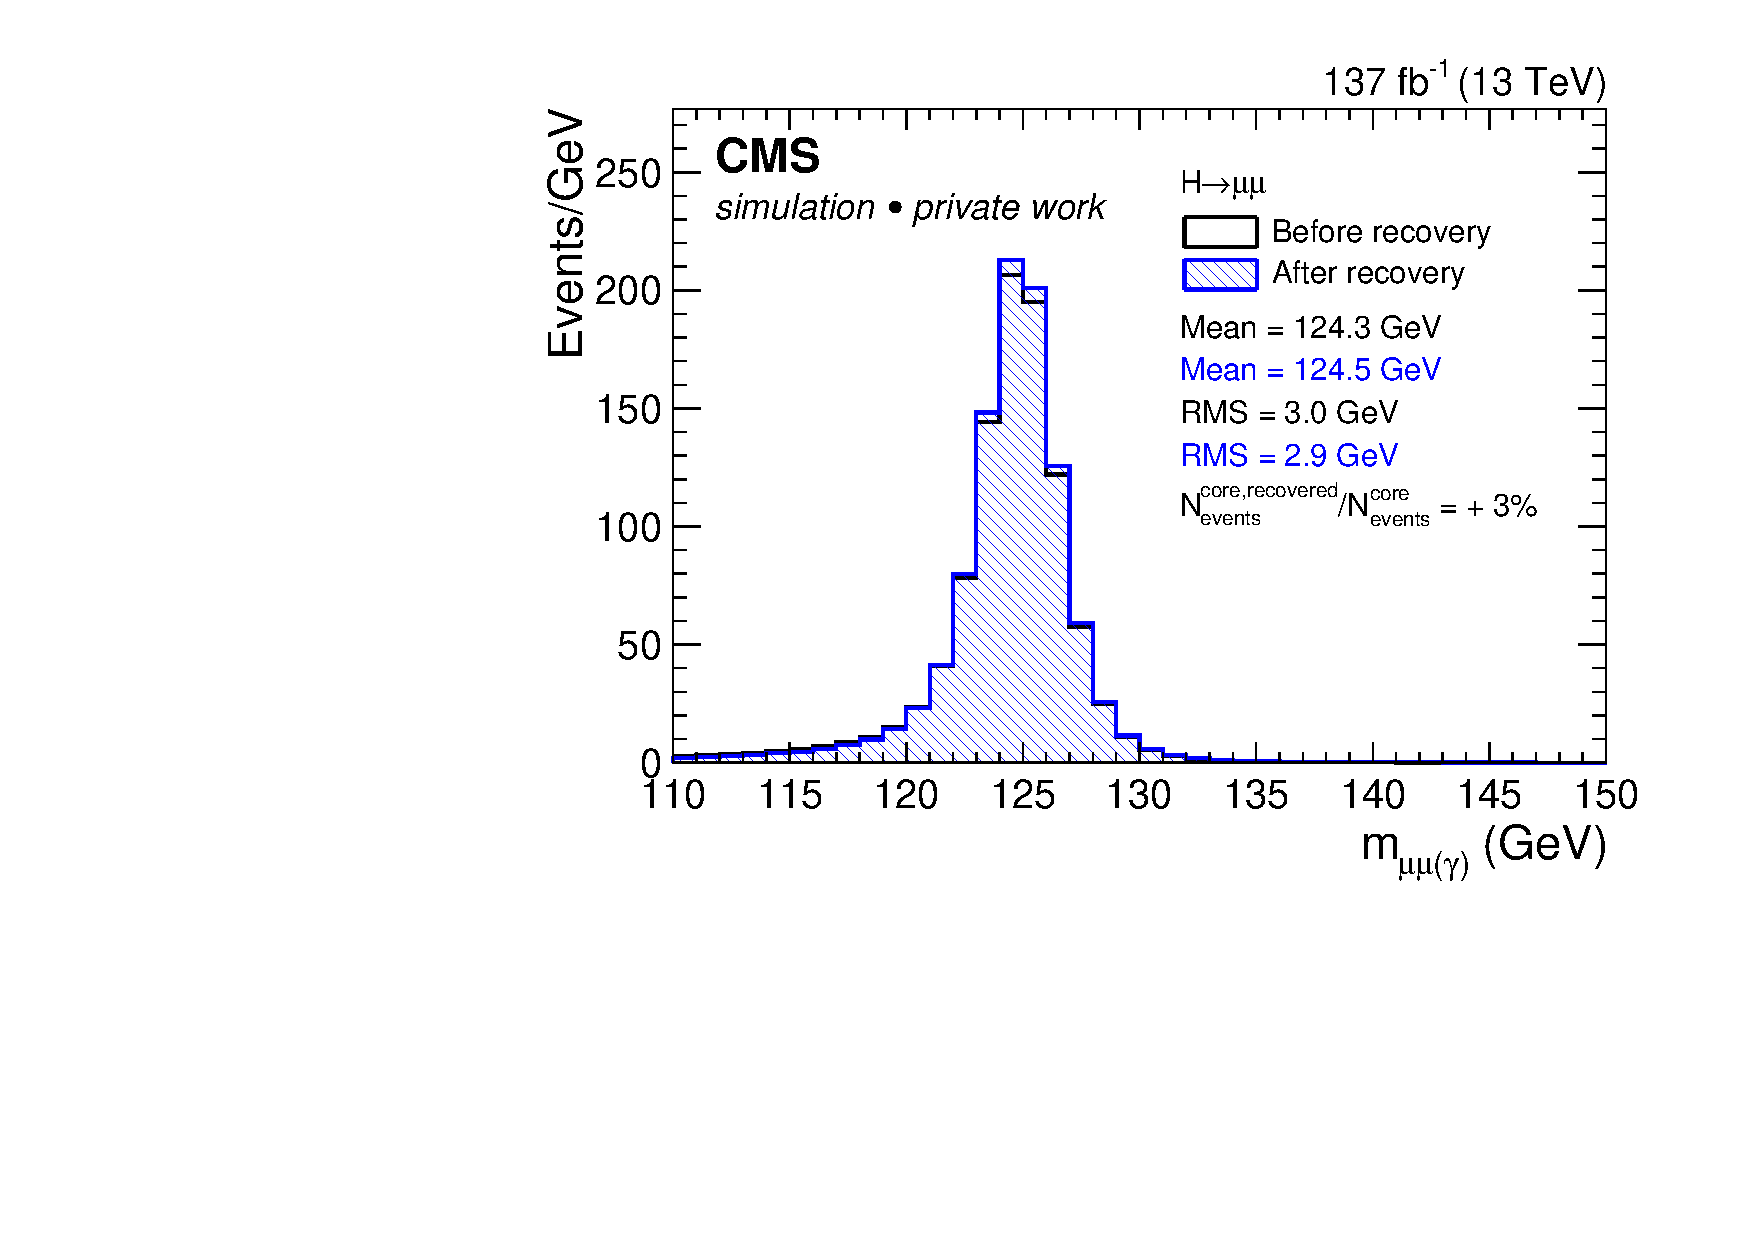
\includegraphics[width=0.45\textwidth]{pics/muon_corr/FSR/FSRrecovery_FullSignal.pdf}
      \caption{Performance of the \FSR in the simulated \hmm events. 
               The \mmm before and after the \FSR are shown for the events that contain at least one FSR photon (left),
               and for the inclusive signal events (right).
               Plot taken from Ref.~\cite{oliverthesis}.}
      \label{fig:fsr_sig}
\end{figure*}

\begin{figure*}[!htb]
      \centering
%      \captionsetup{justification=justified}
      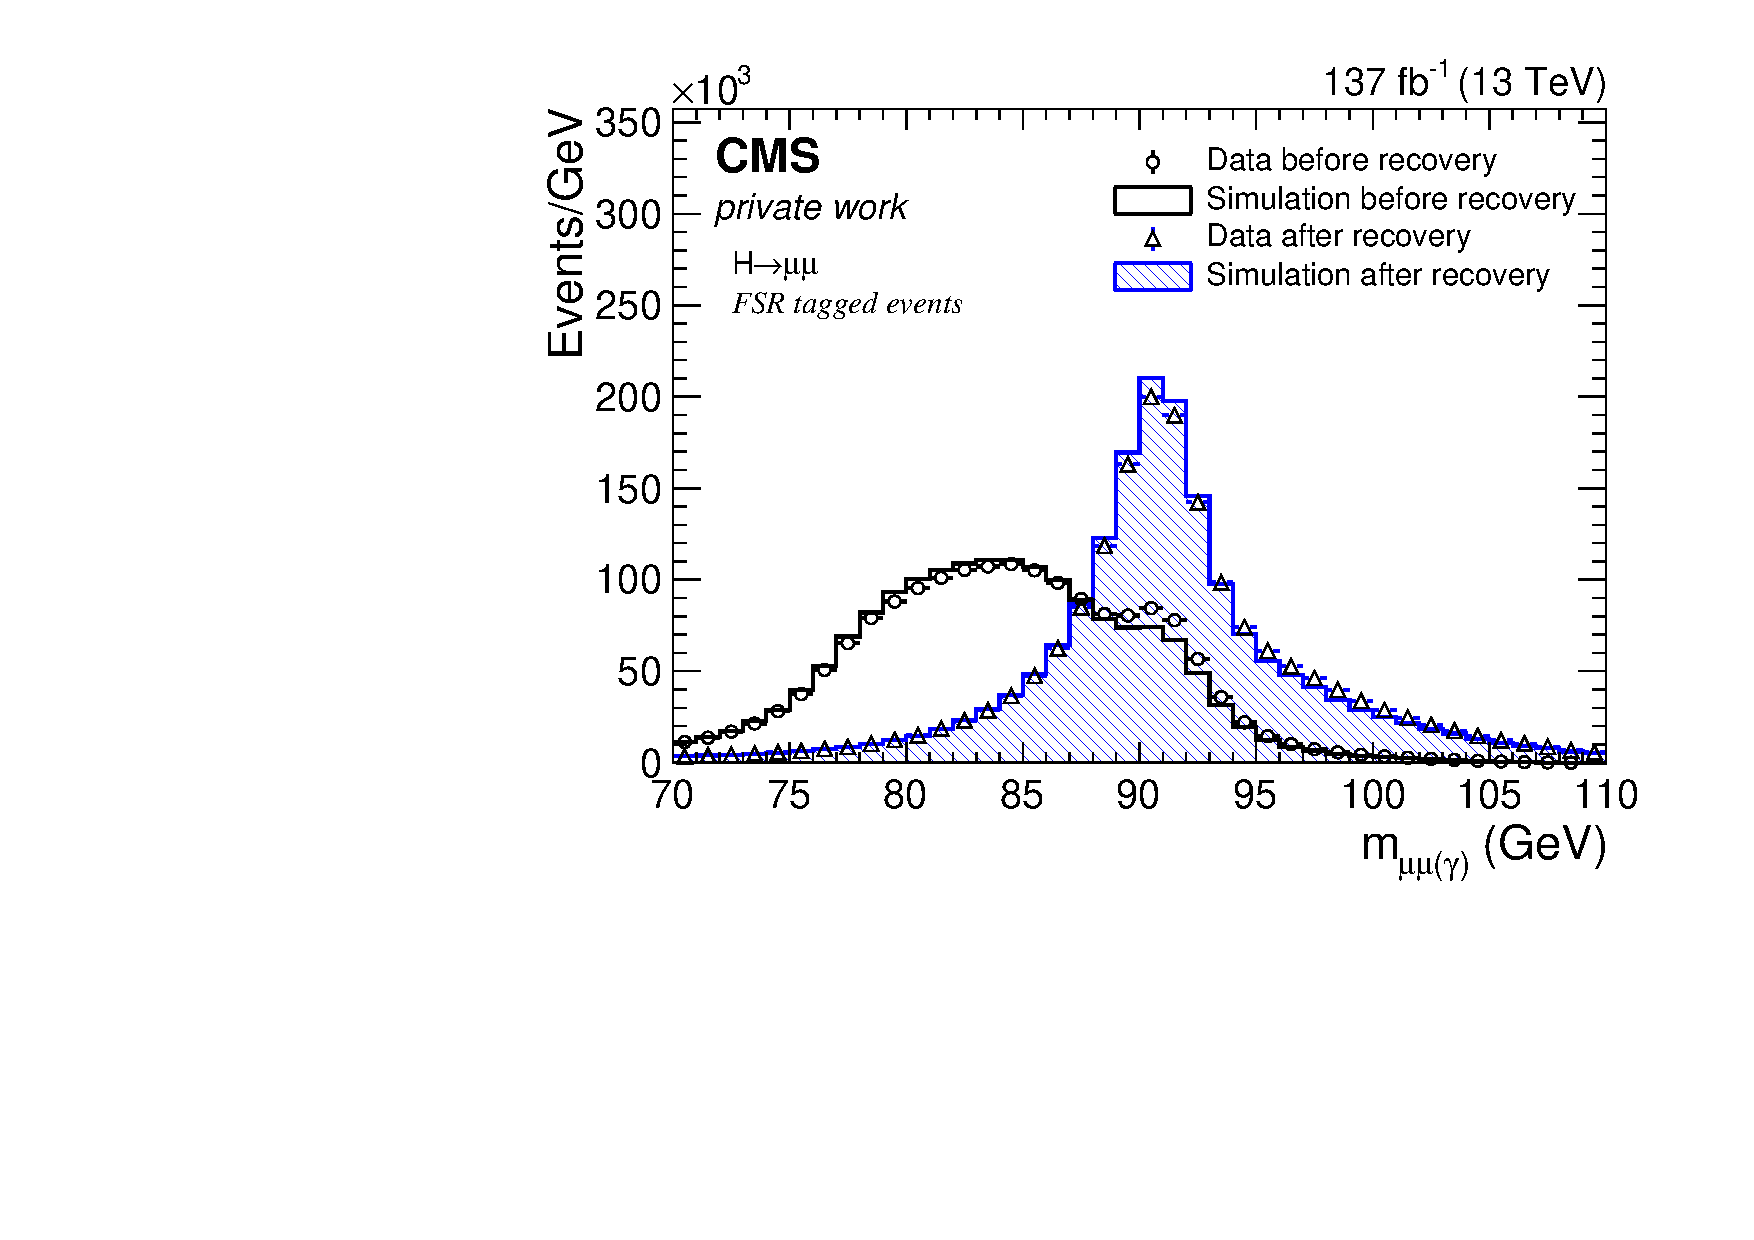
\includegraphics[width=0.45\textwidth]{pics/muon_corr/FSR/FSRrecovery_Validation.pdf}
      \caption{Performance of the \FSR in the \zmm events that contain FSR photons, in both data and simulation. 
               A good agreement between simulation and data is observed, both before and after the correction.
               Plot taken from Ref.~\cite{oliverthesis}.}
      \label{fig:fsr_val}
\end{figure*}


\section{GeoFit Correction} \label{sec:GeoFit}

As described in Section~\ref{sec:reco_track},
tracks are built from hits in silicon trackers and extrapolated to the collision region
without any assumption on their vertices.
Reconstructed tracks may have nonzero displacements from their true origins because of uncertainties in track fits.
If there is a way to locate the true origin of a track, 
it can be used as a constraint on the track to improve the track momentum measurement.
Prompt tracks originate from $pp$ interaction points, 
which are estimated by primary vertices (PV, Section~\ref{sec:reco_pv}) or the beamspot (BS, Section~\ref{sec:reco_bs}).
This section reports the development of a momentum correction for prompt muons (the \GeoFit)
by taking the PV or BS as their true origins.

This correction is based on a geometrical correlation between the \pt mismeasurement 
and the displacement from the reconstructed track to its true vertex.
The correction is applied as a simple analytic function whose parameters are determined from fits to simulations.
It is therefore named the \GeoFit.
Section~\ref{sec:d0_geometry} explains the geometry of the track displacement and the correlation between different variables.
Section~\ref{sec:dev_geofit} describes the studies on simulated samples to find the best fit parameters in that correlation.
The \GeoFit is developed using muon tracks from the $\PZ \to \mu\mu$ process.
It removes the dependence of \mmm on track displacement, which leads to an 
improvement on the \mmm resolution of the combined signal ranging from 3\% to 10\%, depending on the data-taking period.
Details of the \GeoFit performance, along with validation studies are shown in Section~\ref{sec:perf_geofit}.
In addition, an alternative way to correct this \pt bias is to redo the track fit including the colliding vertex as an additional hit in the track, 
which should achieve a more fundamental correction at the cost of more computational resources.
A preliminary study comparing the \GeoFit with the track refit shows the two methods give almost equivalent results,
detailed in Section~\ref{sec:track_refit}.


\subsection{Geometry of the Track Displacement}\label{sec:d0_geometry}

The displacement of a track from a vertex is usually measured as the impact parameters, $d_{xy}$ and $d_{z}$,
which are the signed distances between the vertex and its point of closest approach (PCA) to the track, in the transverse and longitudinal directions.
In CMS, because most studies only care about the transverse impact parameter, 
the PCA is defined as the point on the 2D-projection of the track in the transverse plane that is the closest to the vertex.
Note that the PCA of the 2D-track is not necessarily the 2D-projection of the PCA in the 3D-space. 
The $d_{z}$ is calculated at the 3D-point corresponding to the 2D-PCA, rather than the 3D-PCA.
As the $d_{z}$ is not used in our studies, the term "impact parameter", if not otherwise stated,
refers specifically to the transverse impact parameter $d_{xy}$, also denoted as $d_{0}$.
The definition of $d_0$ can be expressed as 
\begin{equation}\label{eq:d0_def}
  d_0 = -x_{0} \cdot \text{sin}(\phi_{0}) + y_{0} \cdot \text{cos}(\phi_{0})
\end{equation}
where $(x_{0}, y_{0})$ is the coordinate of a point near the vertex in the frame, in which the vertex is at $(0,0)$, 
and $\phi_{0}$ is the azimuthal angle of the track at $(x_{0}, y_{0})$.
A scheme for this definition is shown in Figure~\ref{fig:d0_def}.

\begin{figure*}[!htb]
      \centering
%      \captionsetup{justification=justified}
      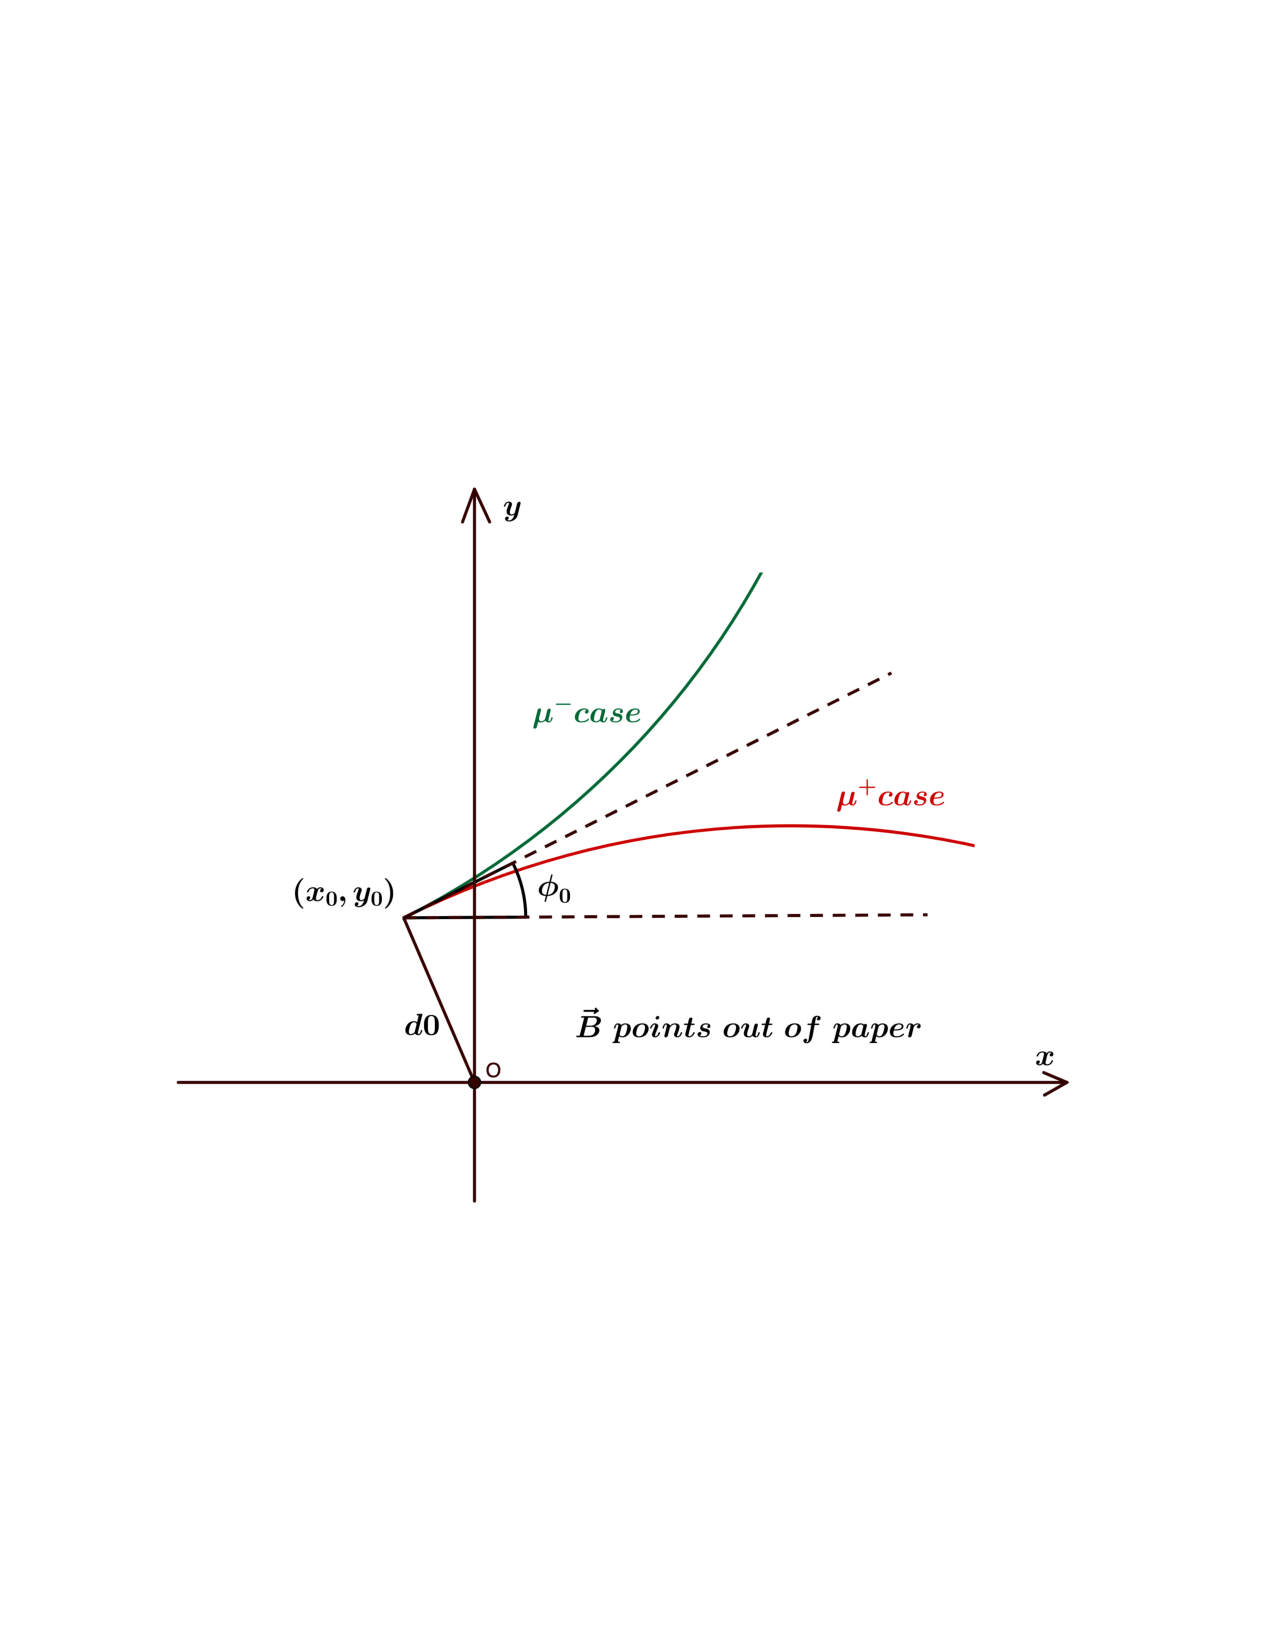
\includegraphics[width=0.70\textwidth]{pics/muon_corr/GeoFit/d0_def.pdf}
      \caption{Scheme of the $d_0$ definition in CMS. The $(x_{0}, y_{0})$ is the coordinate of 
               a point near the vertex in the frame where the vertex is at $(0,0)$, 
               and the $\phi_{0}$ is the azimuthal angle of the track at $(x_{0}, y_{0})$.}
      \label{fig:d0_def}
\end{figure*}

\begin{figure*}[!htb]
      \centering
%      \captionsetup{justification=justified}
      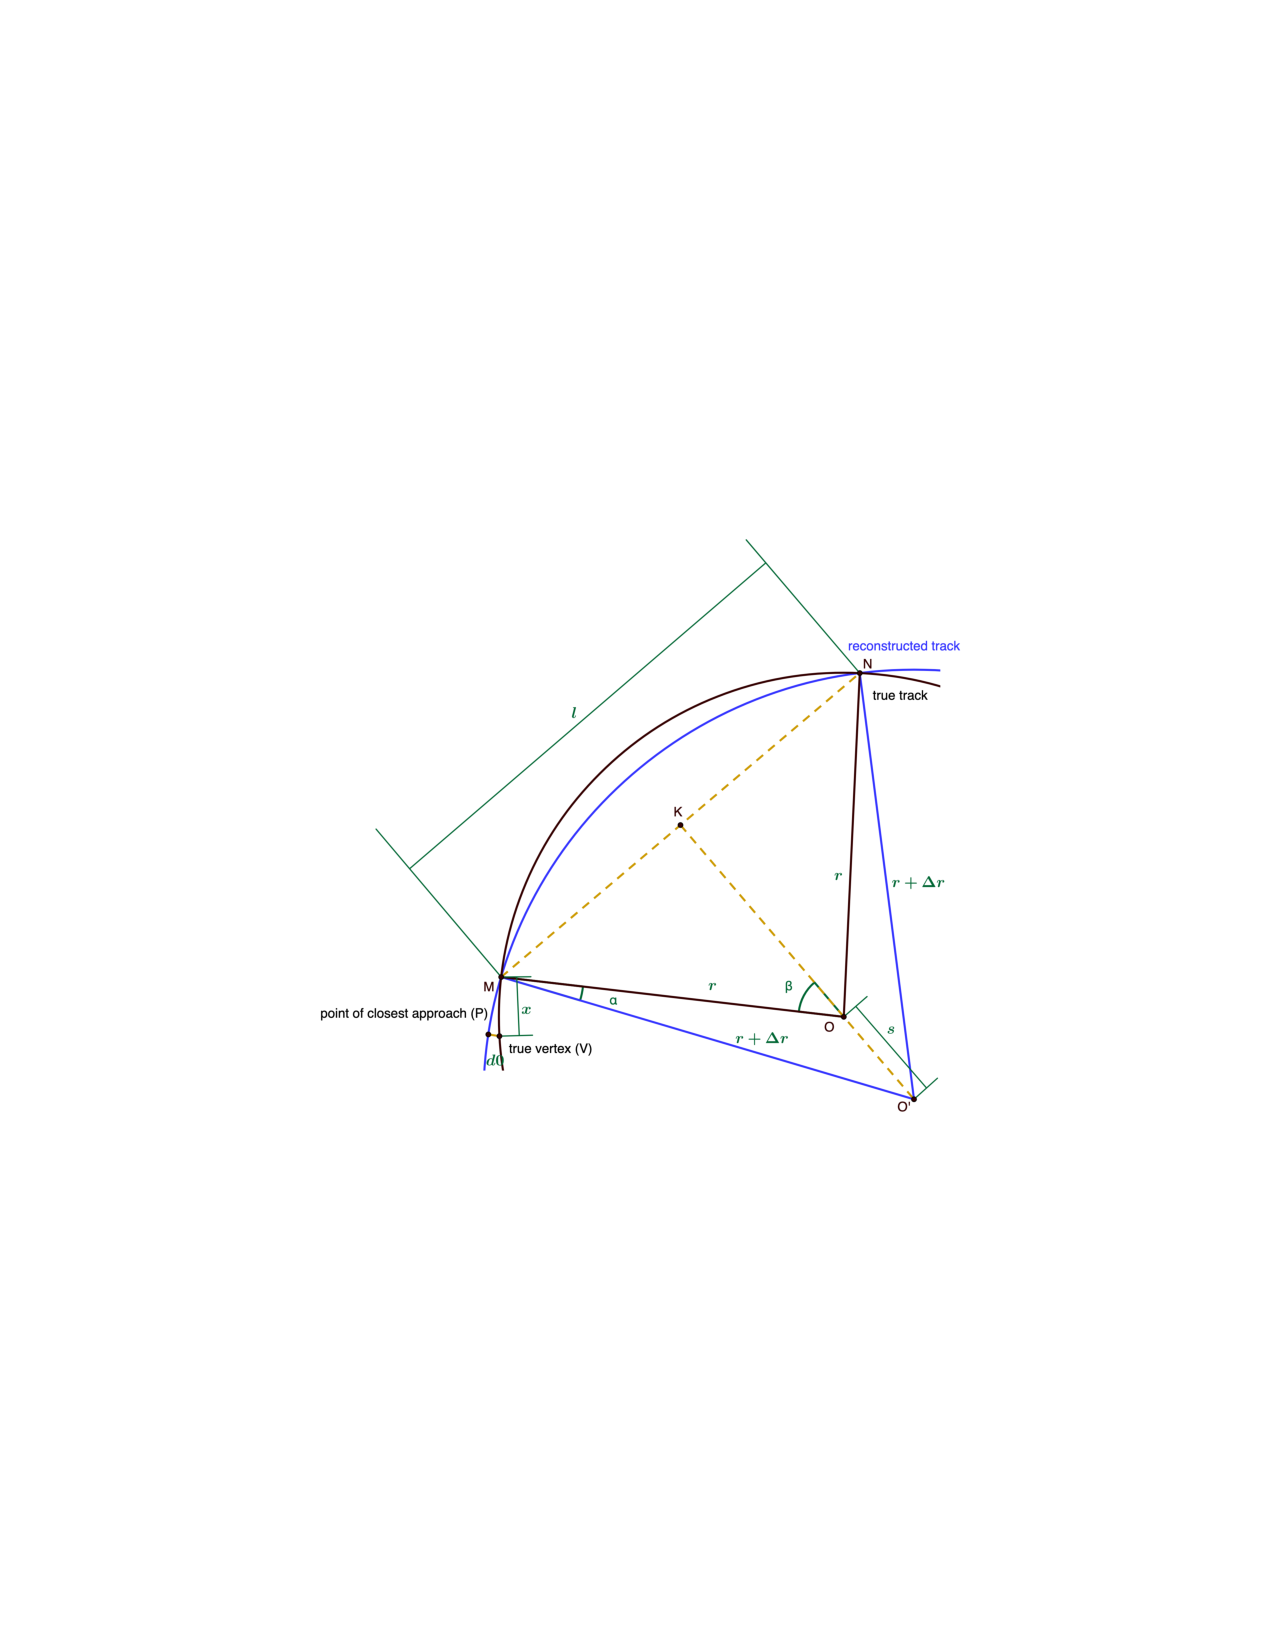
\includegraphics[width=\textwidth]{pics/muon_corr/GeoFit/d0_pt_geometry.pdf}
      \caption{Scheme of the track geometry in the transverse plane. 
               The blue lines show the geometry of the reconstructed track, 
               compared to the black lines, which are the geometry of the true track.
               The difference between the blue track and black track is exaggerated in this scheme.
               The blue track and the black track must intersect at two points.
               $l$ is the distance between the two intersections, 
               and $x$ is the distance between the true vertex and the first intersection.
               $s$ is the distance between the circular centers of the two tracks.}
      \label{fig:d0_pt_scheme}
\end{figure*}

In the track geometry, illustrated in Figure~\ref{fig:d0_pt_scheme}, 
the reconstructed track is very close to, but slightly deviated from, the true track,
which leads to a small $d_0$ between the reco track and the true vertex, 
as well as a small distance between the circular centers of the reco track and the true track.
The circular centers of the two tracks are labels as $O$ and $O'$ for the true track and the reconstructed track,
and $s$ is the distance between $O$ and $O'$. 
The radii of the two tracks are $r$ and $r'$, with $\Delta{}r = r' - r$.
The two circles must intersect at two points, labeled as point $M$ and $N$, 
with the distance between $M$ and $N$ denoted as $l$.
$\beta$ is half of the central angle spanned by the chord $l$ in the true track,
while $\alpha$ is the angle $\angle O'MO$.
The true vertex is denoted as $V$, with $d_0$ as the impact parameter of the reco track to it,
while the PCA on the reco track is denoted as $P$.
The distance between $M$ and $V$ is marked as $x$.
As this scheme represents typical muon tracks in CMS, 
the radii of the tracks under study are at the scale of several tens of meters,
and the $\Delta{}r$ is expected to be much smaller than $r$.
Points $M$ and $N$ are expected to be around the coverage of the CMS tracker system, which is about a meter.
Therefore $x$ and $l$ are expected to be much smaller than $r$ as well.
Finally, the $d_0$ scale of the tracks under study is about ten microns, which is much smaller than $x$, $l$, and $r$. 

In this setup, a few geometrical relationships can be found between different variables, listed as follows:
Since $x \ll r$, arc $\stackrel{\frown}{VM}$ and $\stackrel{\frown}{PM}$ can be viewed as line segments which are respectively perpendicular to $OM$ and $O'M$.
Therefore in triangle $\triangle VMP$, 
\begin{equation}\label{eq:d01}
      d_0 = x \cdot \text{sin}\alpha
\end{equation}      
In triangle $\triangle O'MO$, the sine law gives
\begin{equation}\label{eq:d02}
      \frac{s}{\text{sin}\alpha} = \frac{r+\Delta{}r}{\text{sin}\beta}
\end{equation}
And in triangle $\triangle OMK$, 
\begin{equation}\label{eq:d03}
      \text{sin}\beta = \frac{l/2}{r}
\end{equation}   
Then, using the Pythagorean theorem in both triangle $\triangle O'MK$ and triangle $\triangle OMK$, there is
\begin{equation}\label{eq:d04}
      s =  \sqrt{(r+\Delta{}r)^{2} - (l/2)^{2}} - \sqrt{r^{2} - (l/2)^{2}}
\end{equation}   
Combining Equation ~\ref{eq:d01} to ~\ref{eq:d04} and assuming $r \gg l$, one can get
\begin{equation}\label{eq:d05}
      d_0 = \frac{xl}{2} \cdot \frac{\Delta{}r}{r^{2}}
\end{equation}  
Note that in CMS, under the 3.8T magnetic field, tracks follow 
\begin{equation}
    \pt ~(\text{in ~\GeV}) = 1.14 \cdot r ~(~\text{in meter})   
\end{equation}
We reach
\begin{equation}\label{eq:d0_prop}
    d_0 \propto \frac{\Delta{}\pt}{\pt^{2}}
\end{equation}

Now a quantitative relationship is extracted between $d_0$ and \pt, but with one caveat:
the variables $x$ and $l$ in the scheme above may vary track by track, and are impossible to measure in real data,
meaning that the coefficient in the proportionality is not a constant for different tracks, and Equation~\ref{eq:d0_prop} can be smeared.
Therefore, to validate this proportionality, studies are performed on simulated samples comparing the reconstructed \pt and the generated \pt of muon tracks.
Plots of $(\pt^{reco}-\pt^{gen})/ (\pt^{gen})^{2}$ vs $d_0$ are made, 
to see whether the proportionality can be observed after the smearing,
which is the topic of Section~\ref{sec:dev_geofit}.

Another remark needs to be made, that in Figure~\ref{fig:d0_pt_scheme} the \pt mismeasurement is related to the relative position of the true vertex to the reconstructed track.
To be more specific, if the true vertex is inside of the reco track, the \pt is overestimated, 
while if the true vertex is outside of the reco track, the \pt is underestimated. 
However, in the CMS definition of $d_0$ shown in Figure~\ref{fig:d0_def}, the sign of $d_0$ corresponds to an opposite relative position between the vertex and the track
for the positively charged muons and the negatively charged muons. 
A positive $d_0$ value means the true vertex is inside of the reco track if the muon is positive, but outside of the reco track if the muon is negative.
Therefore in CMS convention the $d_0-\pt$ correlation is expected be reversed for different muon charges,
and in Section~\ref{sec:dev_geofit} studies are always performed evaluating $d_0 \times$ charge rather than just $d_0$.

\subsection{Development of GeoFit}\label{sec:dev_geofit}

The $(\pt^{reco}-\pt^{gen})/ (\pt^{gen})^{2}$ vs $d_0$ plots are made with the following steps:
The values $\pt^{reco}$, $\pt^{gen}$, and $d_0$ are extracted for each track in simulated samples.
The distribution of $(\pt^{reco}-\pt^{gen})/ (\pt^{gen})^{2}$ is made for tracks in different $d_0 \times$ charge bins.
The maximum position and the corresponding full-width-half-maximum (FWHM) is found for each 
fine-binned $(\pt^{reco}-\pt^{gen})/ (\pt^{gen})^{2}$ distribution and set as the value and the uncertainty
of one data point in the plots in Figure~\ref{fig:pv_vs_bs_fits}.
The plots are then fit with analytic functions, which are considered as the experimental realization of Equation~\ref{eq:d0_prop}.

In CMS, the colliding vertex is measured by two physics objects, 
the primary vertex (PV) and the beamspot (BS), as described in Sections~\ref{sec:reco_pv} and ~\ref{sec:reco_bs}.
Both vertex types are tested and compared in the development of \GeoFit.
Examples of the corresponding $(\pt^{reco}-\pt^{gen})/ (\pt^{gen})^{2}$ vs $d_0$ dependences are shown in Figure~\ref{fig:pv_vs_bs_fits}.
The dependence in the PV plot is not linear as the reconstructed PV is pulled towards the energetic muon tracks,
while the dependence in the BS plot follows a linear trend as predicted in Equation~\ref{eq:d0_def}.
This is understood as the PV position, reconstructed with a limited number of tracks, 
can be biased toward the few energetic tracks associated to it, 
while the BS, averaging numerous tracks from many events, is less affected by individual tracks.
Therefore the BS is considered as the position of the true vertex in the rest of the study.


\begin{figure*}[!htb]
      \centering
%      \captionsetup{justification=justified}
      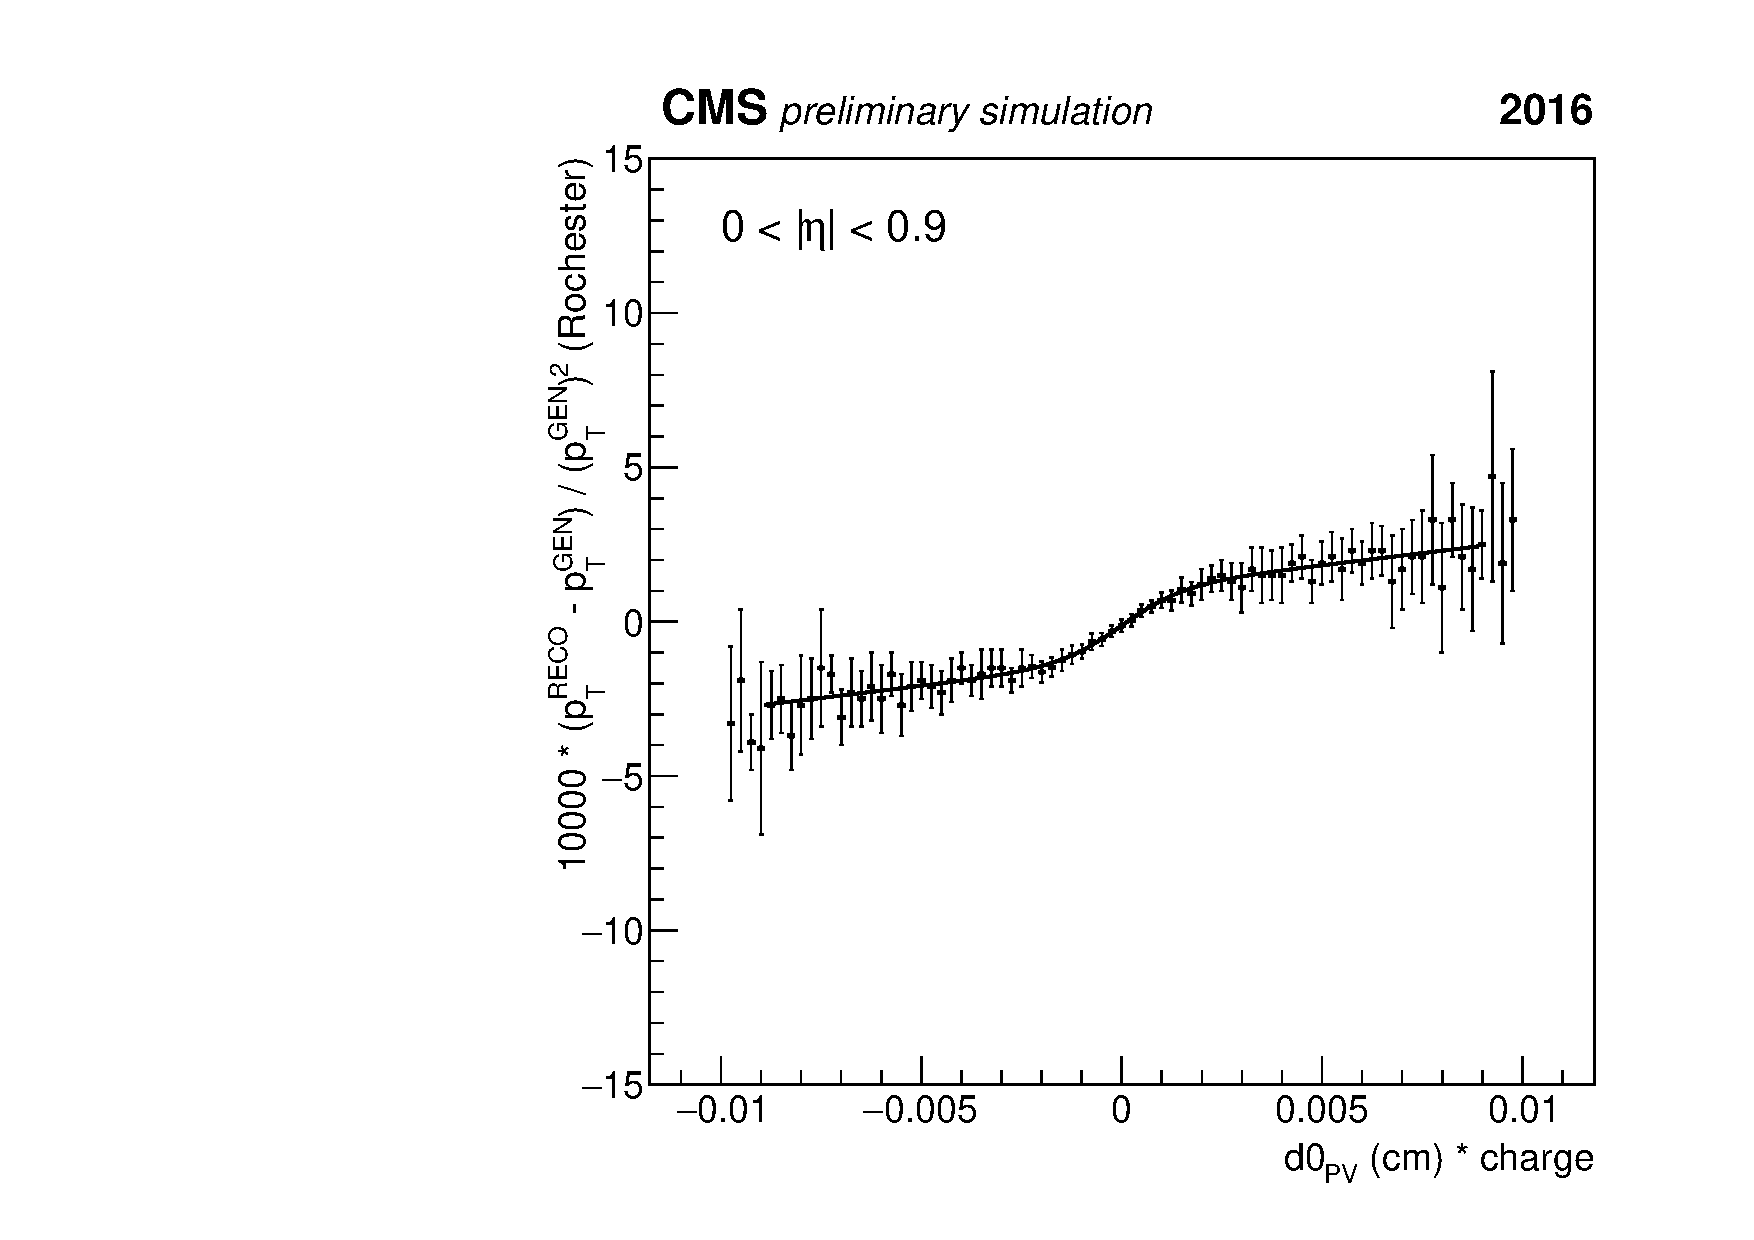
\includegraphics[width=0.45\textwidth]{pics/muon_corr/GeoFit/fit_results/d0_pt_PV_eg.pdf}
      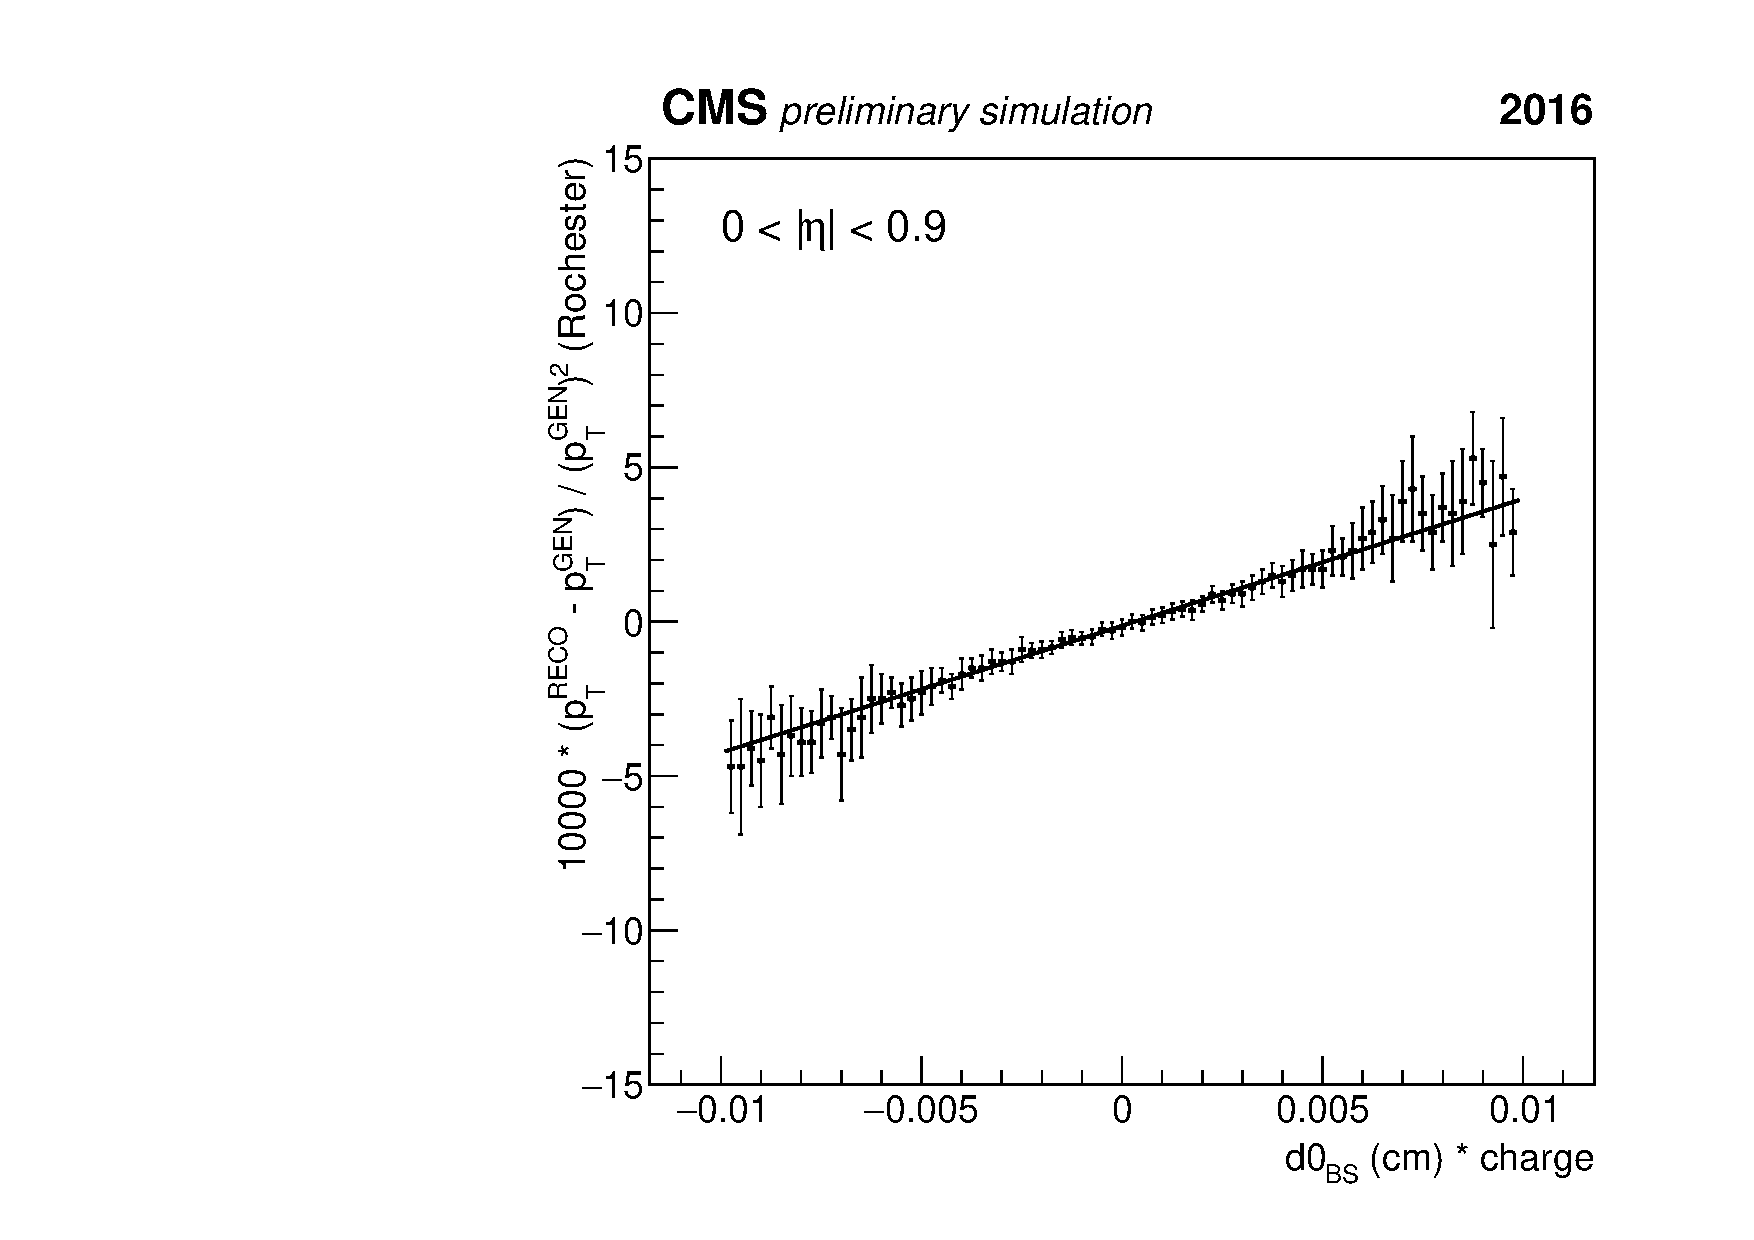
\includegraphics[width=0.45\textwidth]{pics/muon_corr/GeoFit/fit_results/d0_pt_BS_eg.pdf}
      \caption{Example plots showing the correlation between $(\pt^{reco}-\pt^{gen})/ (\pt^{gen})^{2}$ and $d_0 \times$ charge.
               The vertices used for the $d_0$ calculation are the PV (left) and the BS (right). 
               The PV plot shows a modulated dependence from expectation while the BS plot shows a linear shape as expected.
               Only barrel tracks from 2016 data are shown as examples. 
               Plots of other |\eta| regions and other data-taking periods show a similar behavior.
               Plots credit to Efe Yigitbasi.}
      \label{fig:pv_vs_bs_fits}
\end{figure*}

The $(\pt^{reco}-\pt^{gen})/ (\pt^{gen})^{2}$ vs $d_0$ correlation is found to be different in different |\eta| regions and data-taking periods: 
different |\eta| regions are covered by different detector components, and there have been upgrades on the detector and the reconstruction algorithm between different data-taking periods.
Overall, the $(\pt^{reco}-\pt^{gen})/ (\pt^{gen})^{2}$ vs $d_0$ correlation is evaluated by three years (2016, 2017, 2018) and 
three |\eta| regions (barrel, overlap, endcap), shown in Figure~\ref{fig:geofit_param_2016} for 2016, ~\ref{fig:geofit_param_2017} for 2017, and ~\ref{fig:geofit_param_2018} for 2018.
Each of the plots is fit with a linear function, whose best fit parameters are also shown in the plot.

\begin{figure*}[!htb]
      \centering
%      \captionsetup{justification=justified}
      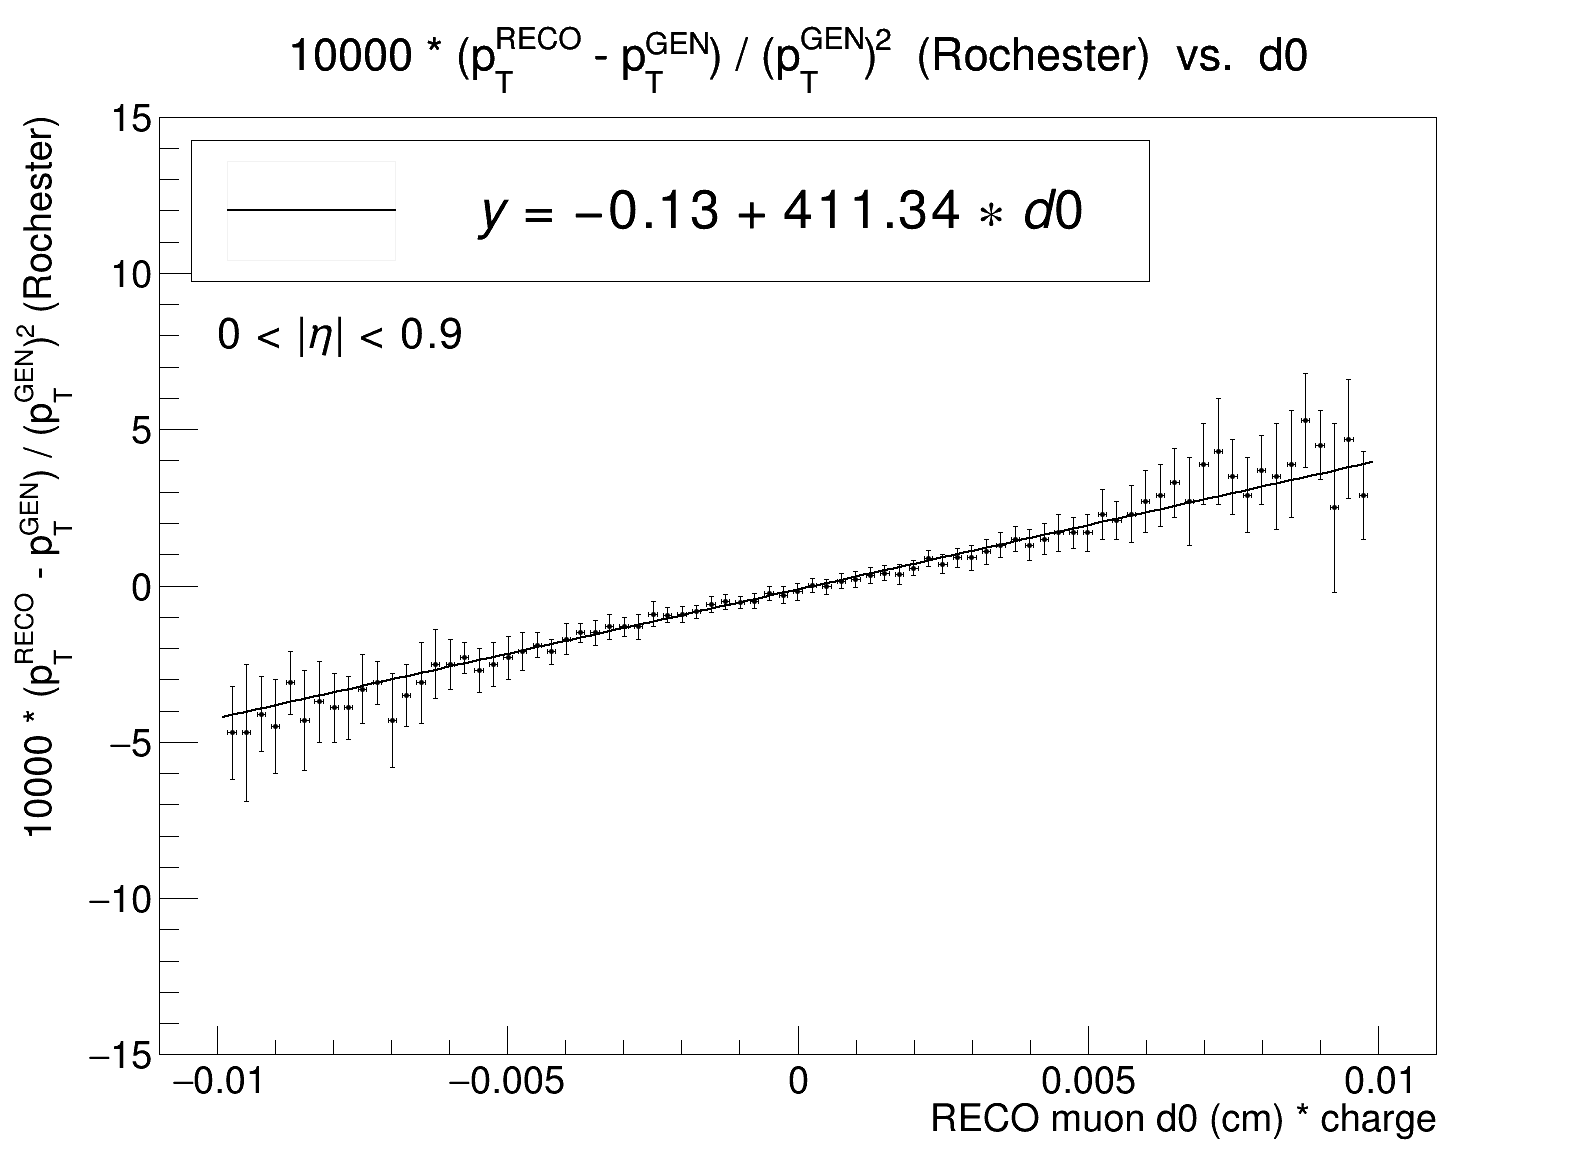
\includegraphics[width=0.32\textwidth]{pics/muon_corr/GeoFit/fit_results/2016_DY_eta_0_0p9_dRelPt2p0_Roch.png}
      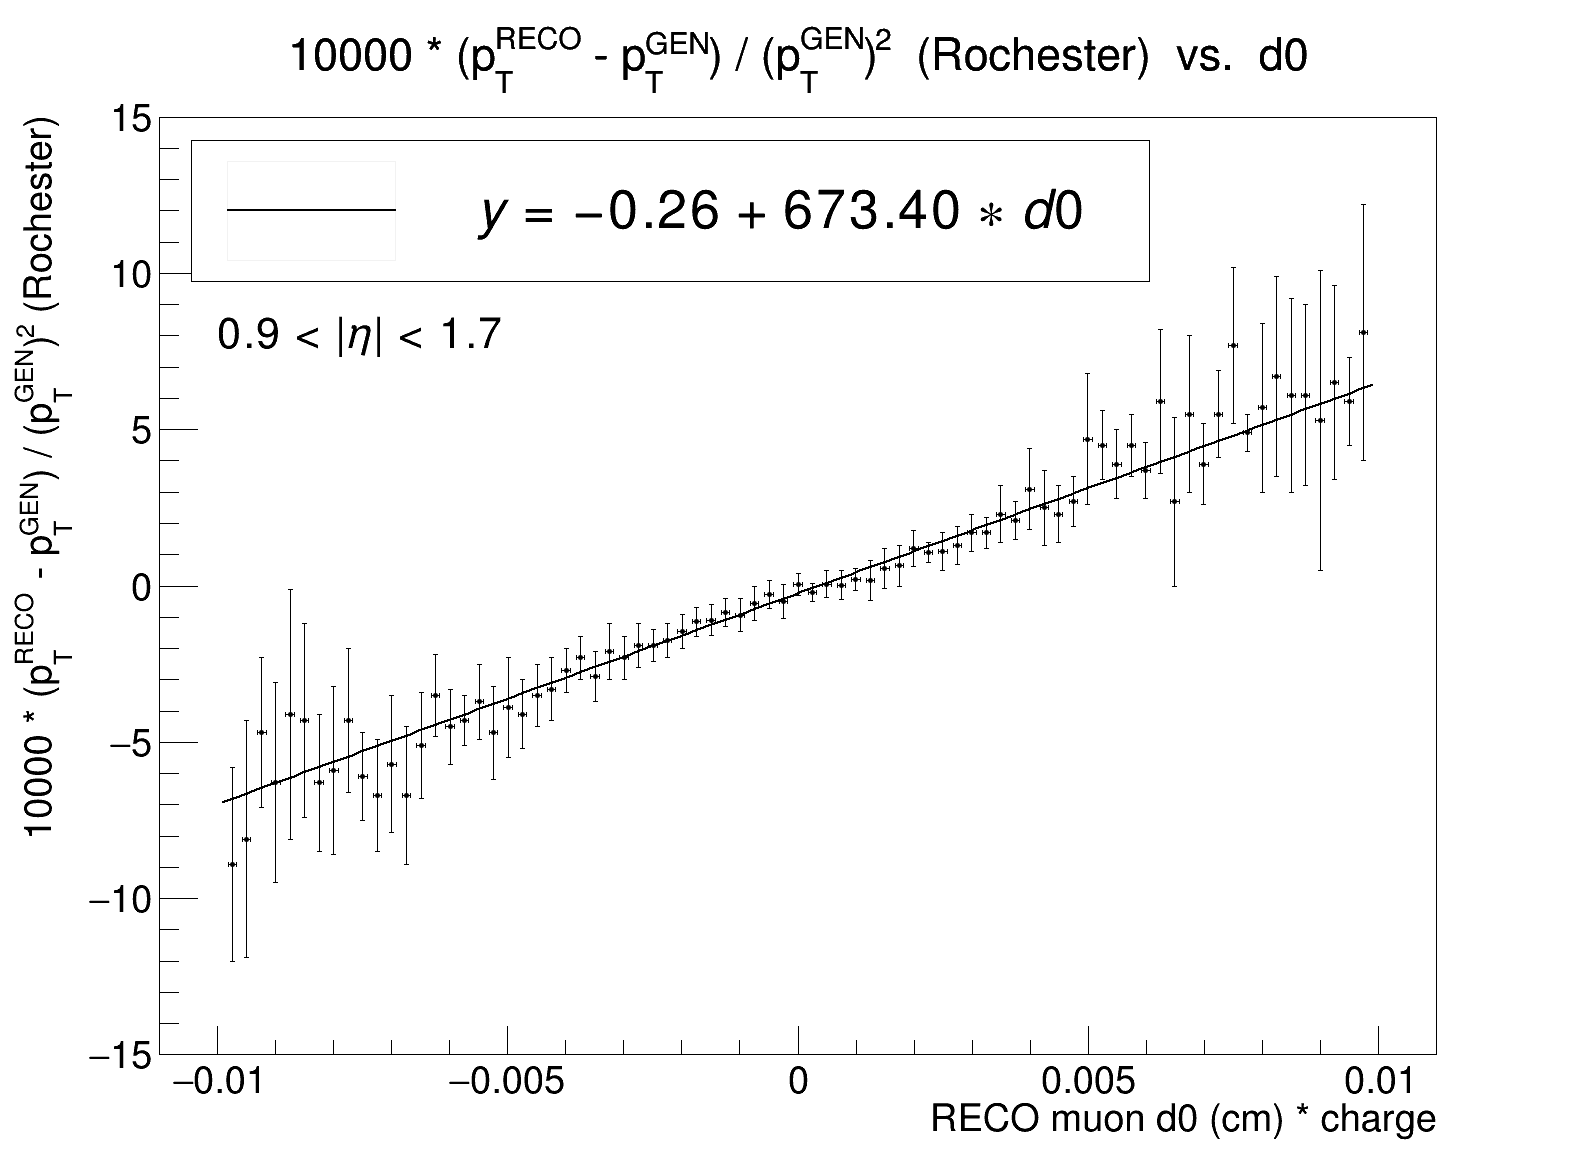
\includegraphics[width=0.32\textwidth]{pics/muon_corr/GeoFit/fit_results/2016_DY_eta_0p9_1p7_dRelPt2p0_Roch.png}
      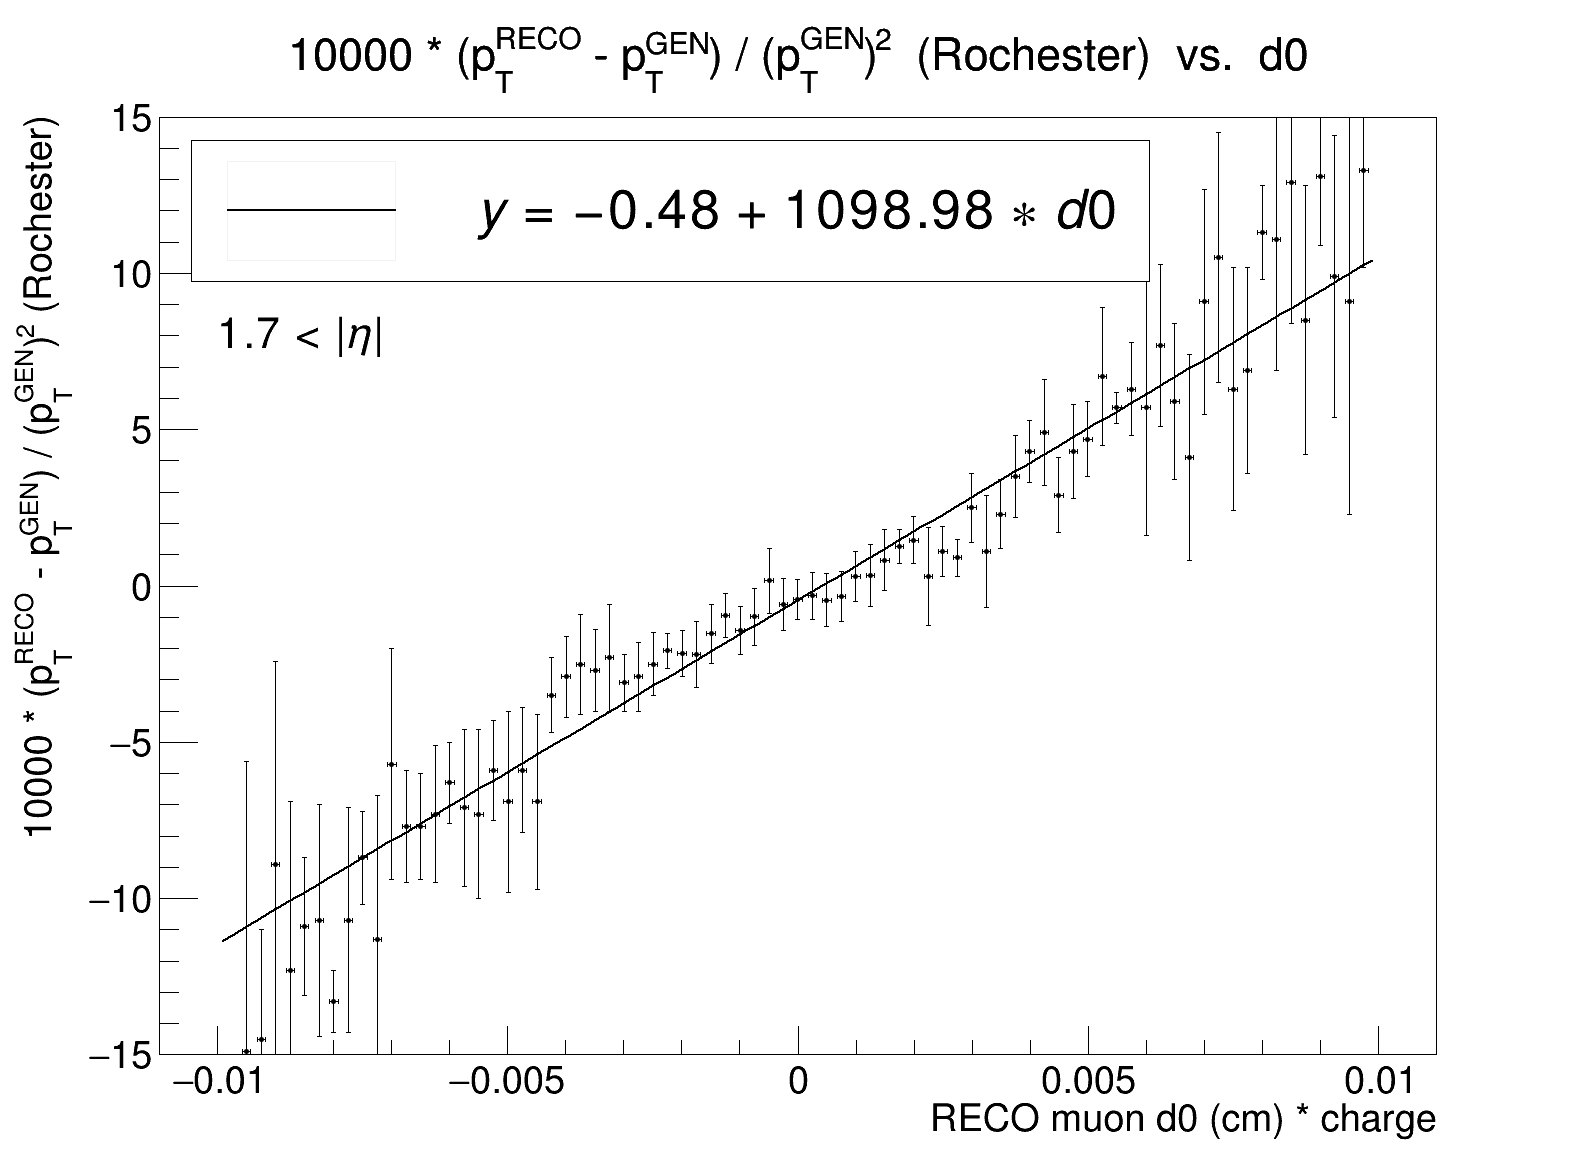
\includegraphics[width=0.32\textwidth]{pics/muon_corr/GeoFit/fit_results/2016_DY_eta_1p7_inf_dRelPt2p0_Roch.png}
      \caption{Plots for the $(\pt^{reco}-\pt^{gen})/ (\pt^{gen})^{2}$ vs $d_0$ correlation in the 2016 \DY simulation, 
               and the linear fits to them. Muon tracks are divided into three different |\eta| regions:
               $|\eta| <$ 0.9 (left), 0.9 $< |\eta| <$ 1.7 (middle), and 1.7 $< |\eta|$ (right).
               Plots credit to Efe Yigitbasi.}
      \label{fig:geofit_param_2016}
\end{figure*}

\begin{figure*}[!htb]
      \centering
%      \captionsetup{justification=justified}
      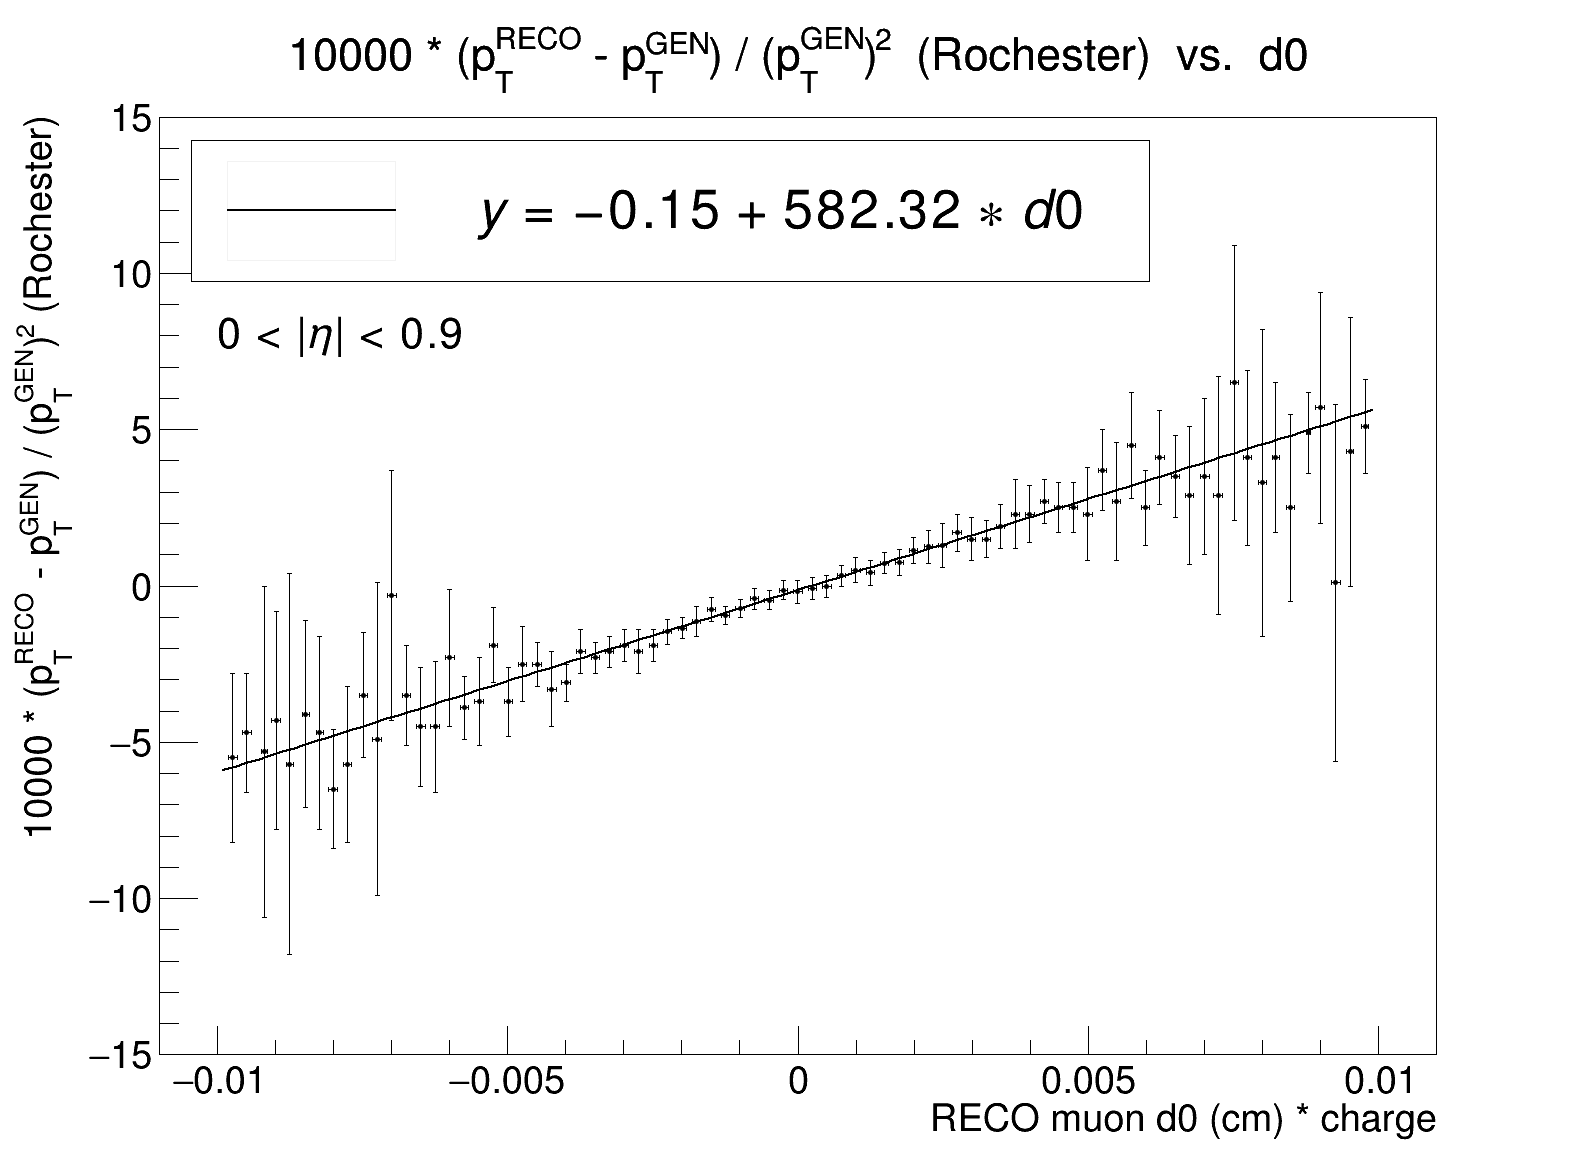
\includegraphics[width=0.32\textwidth]{pics/muon_corr/GeoFit/fit_results/2017_DY_eta_0_0p9_dRelPt2p0_Roch.png}
      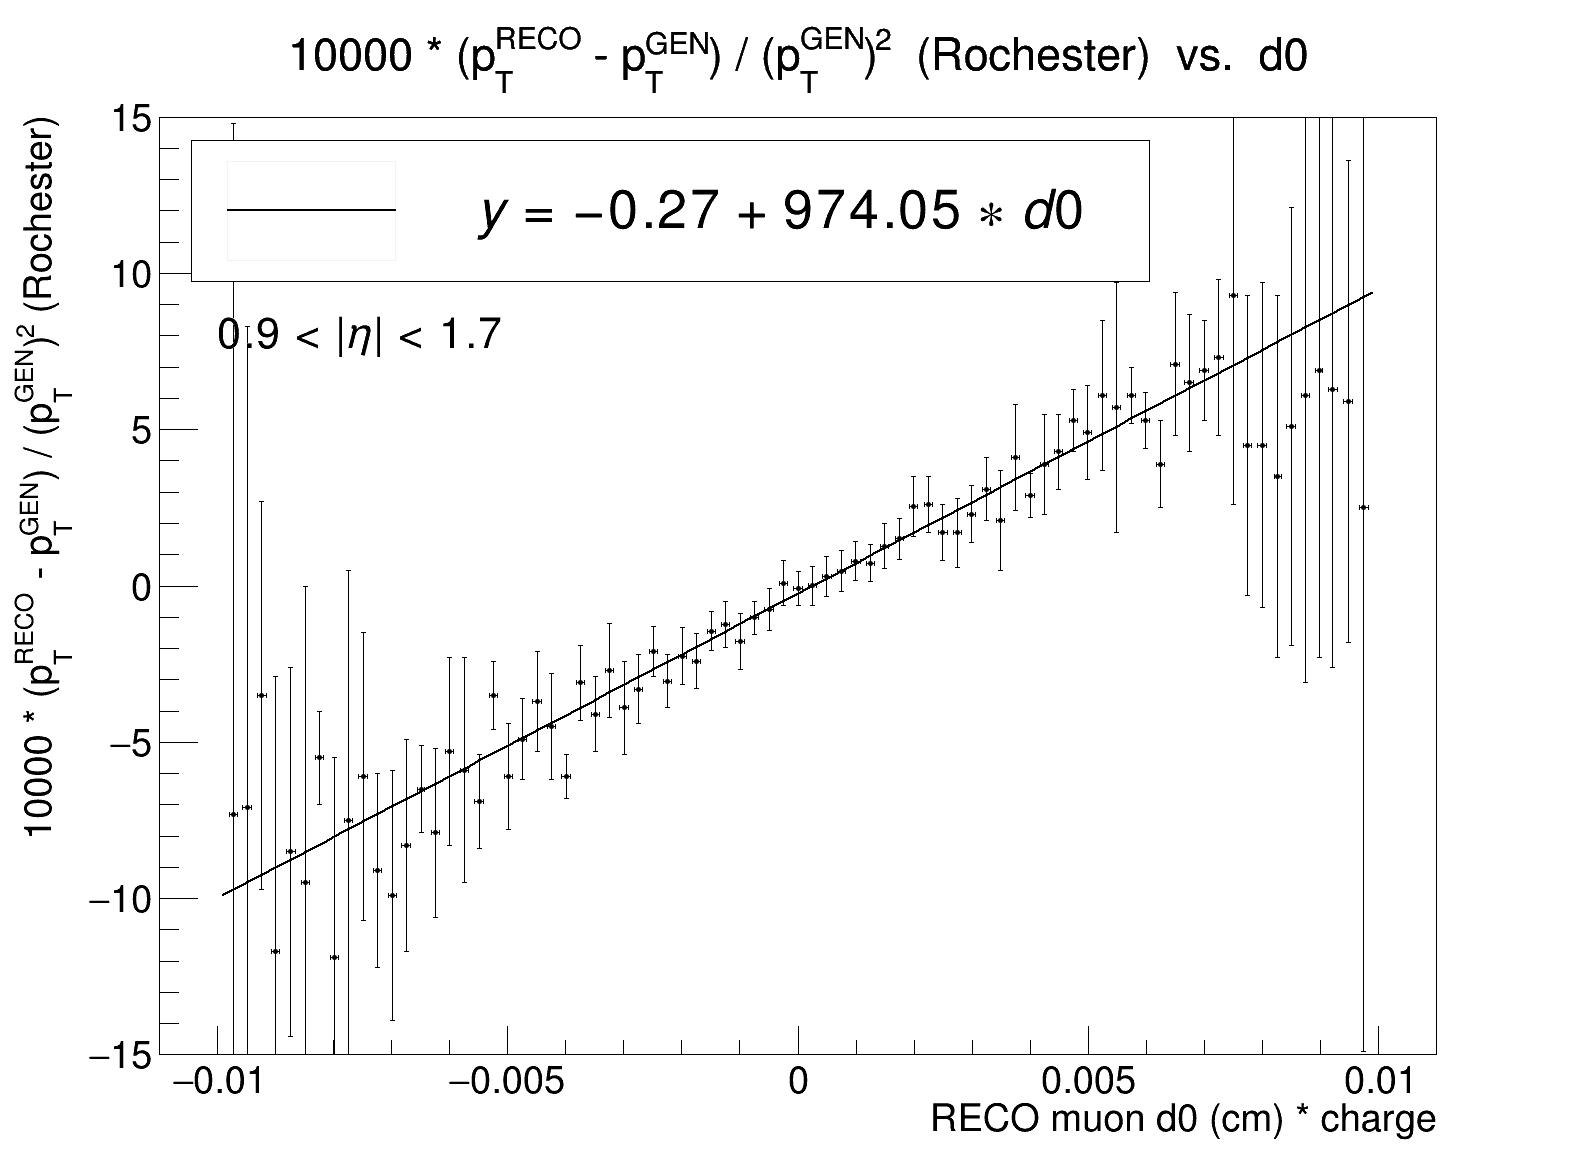
\includegraphics[width=0.32\textwidth]{pics/muon_corr/GeoFit/fit_results/2017_DY_eta_0p9_1p7_dRelPt2p0_Roch.png}
      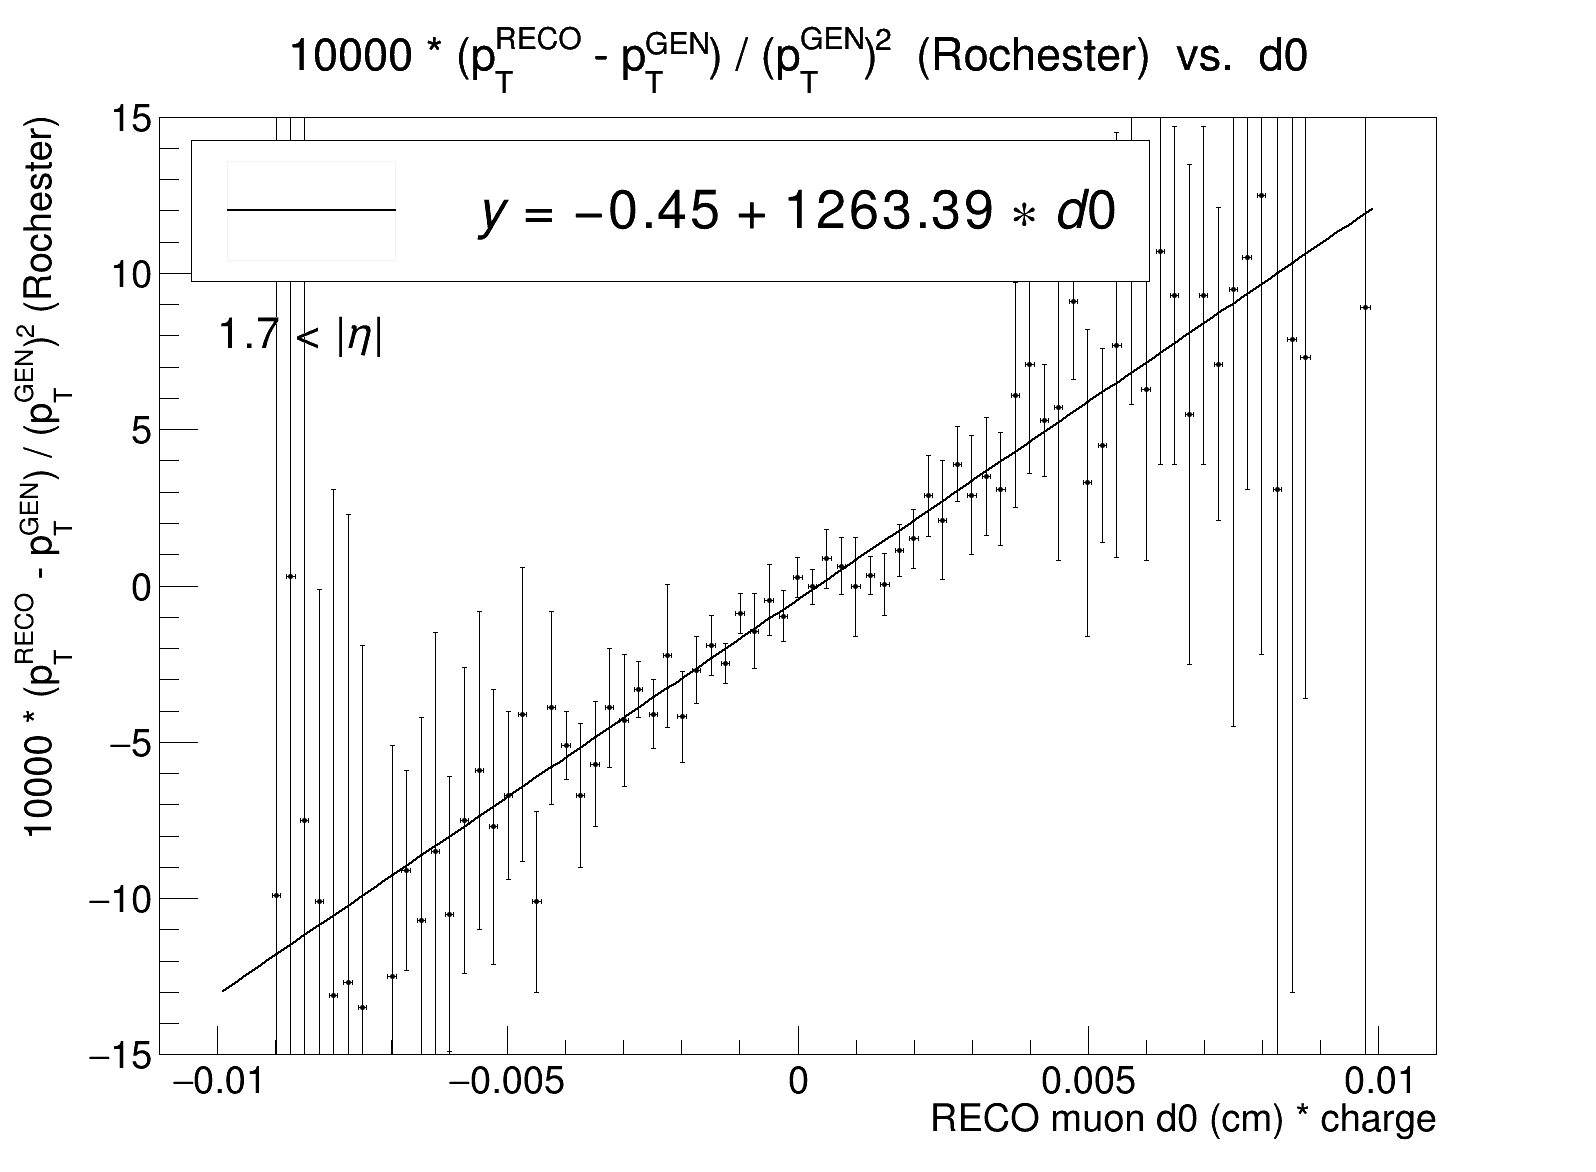
\includegraphics[width=0.32\textwidth]{pics/muon_corr/GeoFit/fit_results/2017_DY_eta_1p7_inf_dRelPt2p0_Roch.png}
      \caption{Plots for the $(\pt^{reco}-\pt^{gen})/ (\pt^{gen})^{2}$ vs $d_0$ correlation in the 2017 \DY simulation, 
               and the linear fits to them. Muon tracks are divided into three different |\eta| regions:
               $|\eta| <$ 0.9 (left), 0.9 $< |\eta| <$ 1.7 (middle), and 1.7 $< |\eta|$ (right).
               Plots credit to Efe Yigitbasi.}
      \label{fig:geofit_param_2017}
\end{figure*}

\begin{figure*}[!htb]
      \centering
%      \captionsetup{justification=justified}
      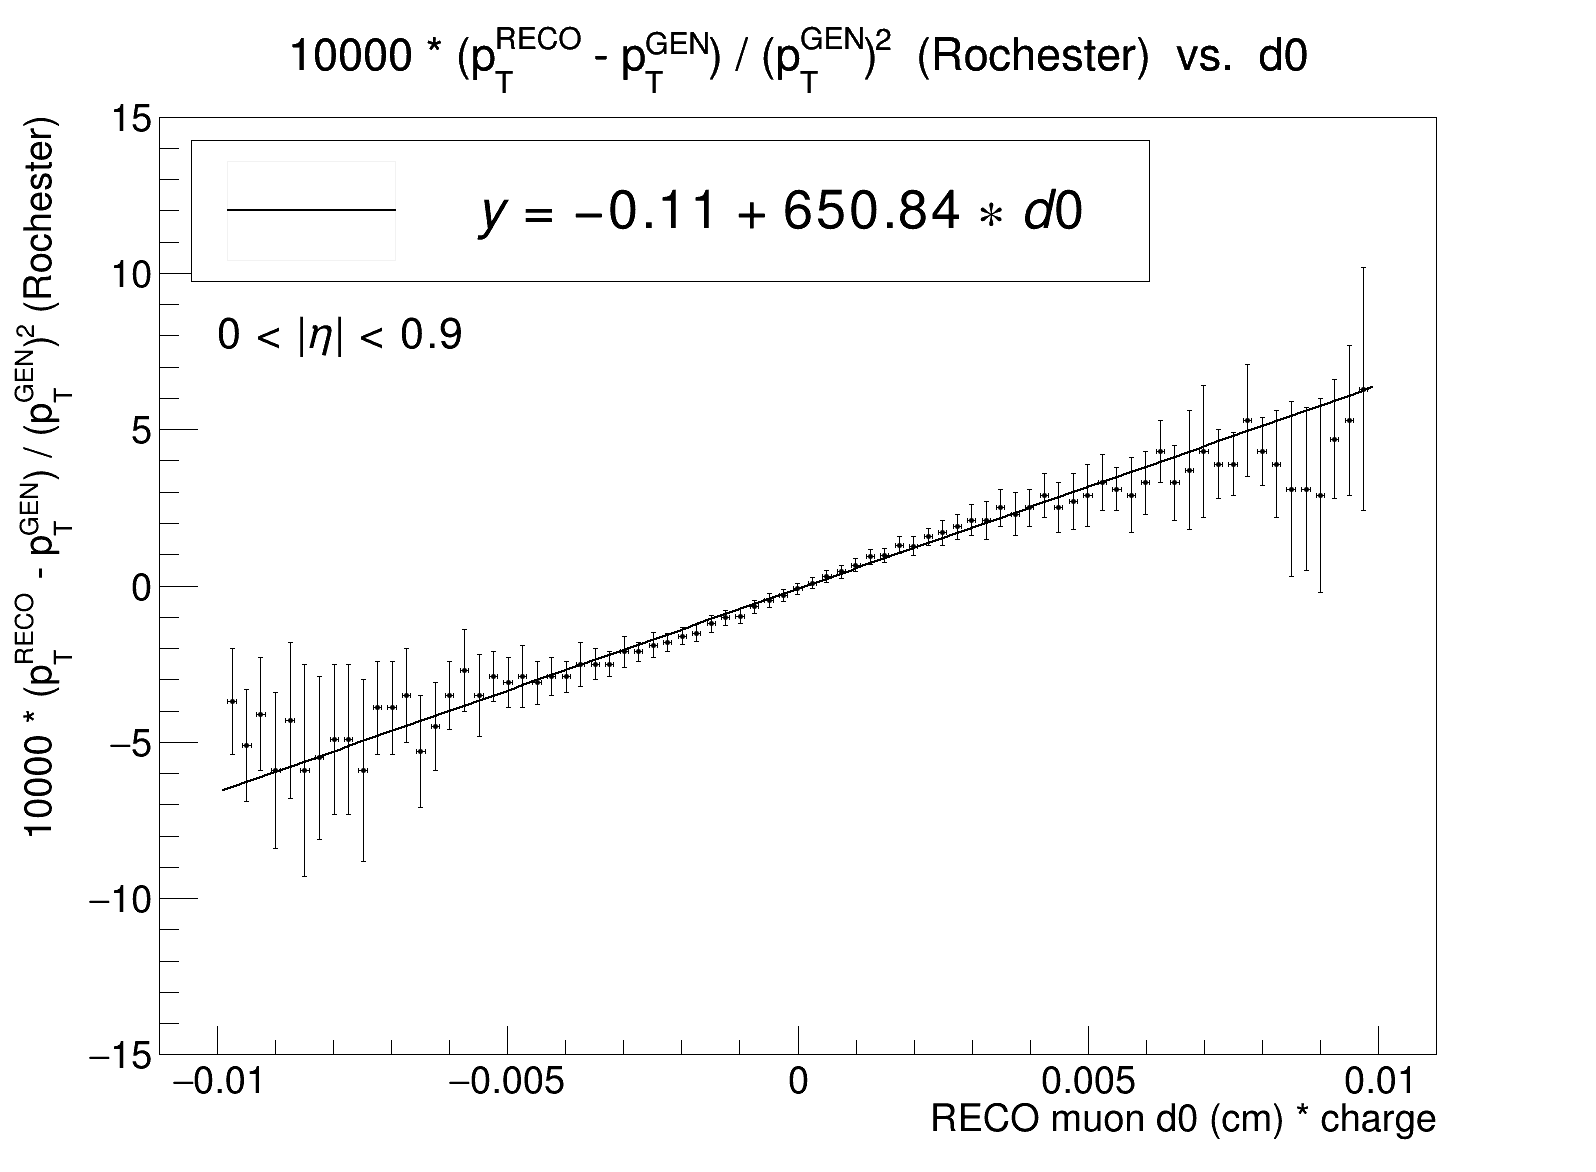
\includegraphics[width=0.32\textwidth]{pics/muon_corr/GeoFit/fit_results/2018_DY_eta_0_0p9_dRelPt2p0_Roch.png}
      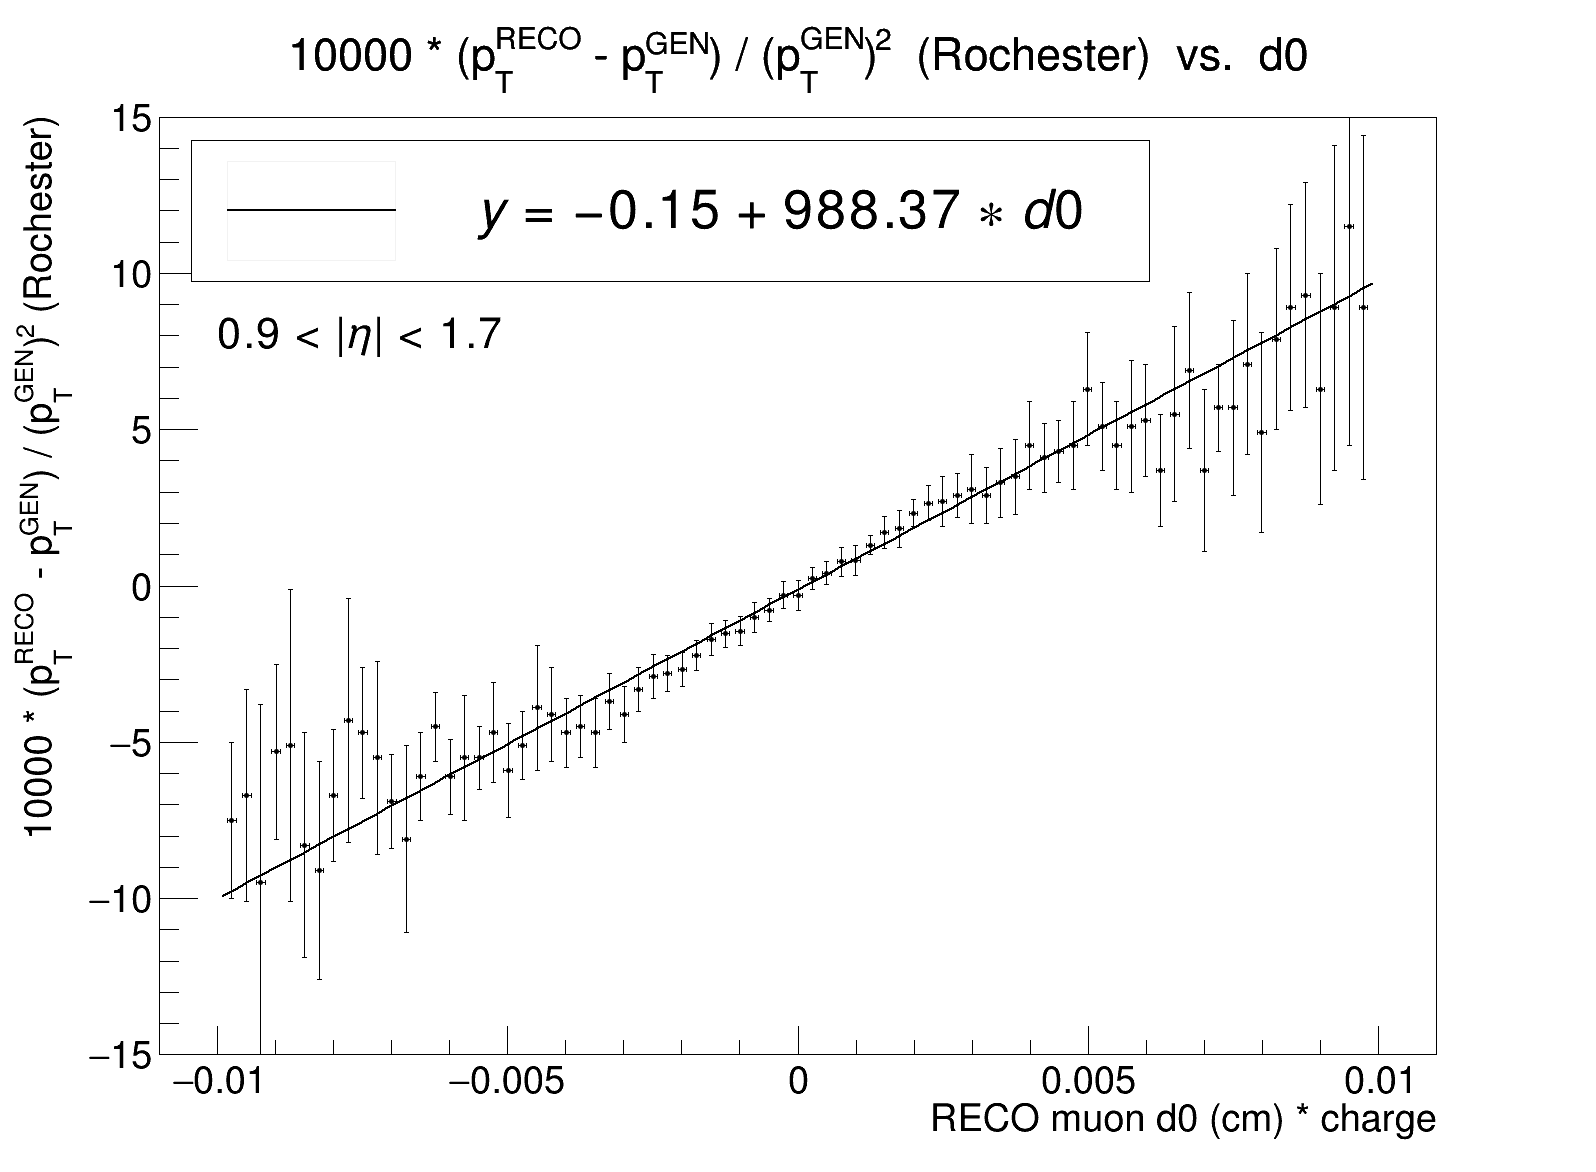
\includegraphics[width=0.32\textwidth]{pics/muon_corr/GeoFit/fit_results/2018_DY_eta_0p9_1p7_dRelPt2p0_Roch.png}
      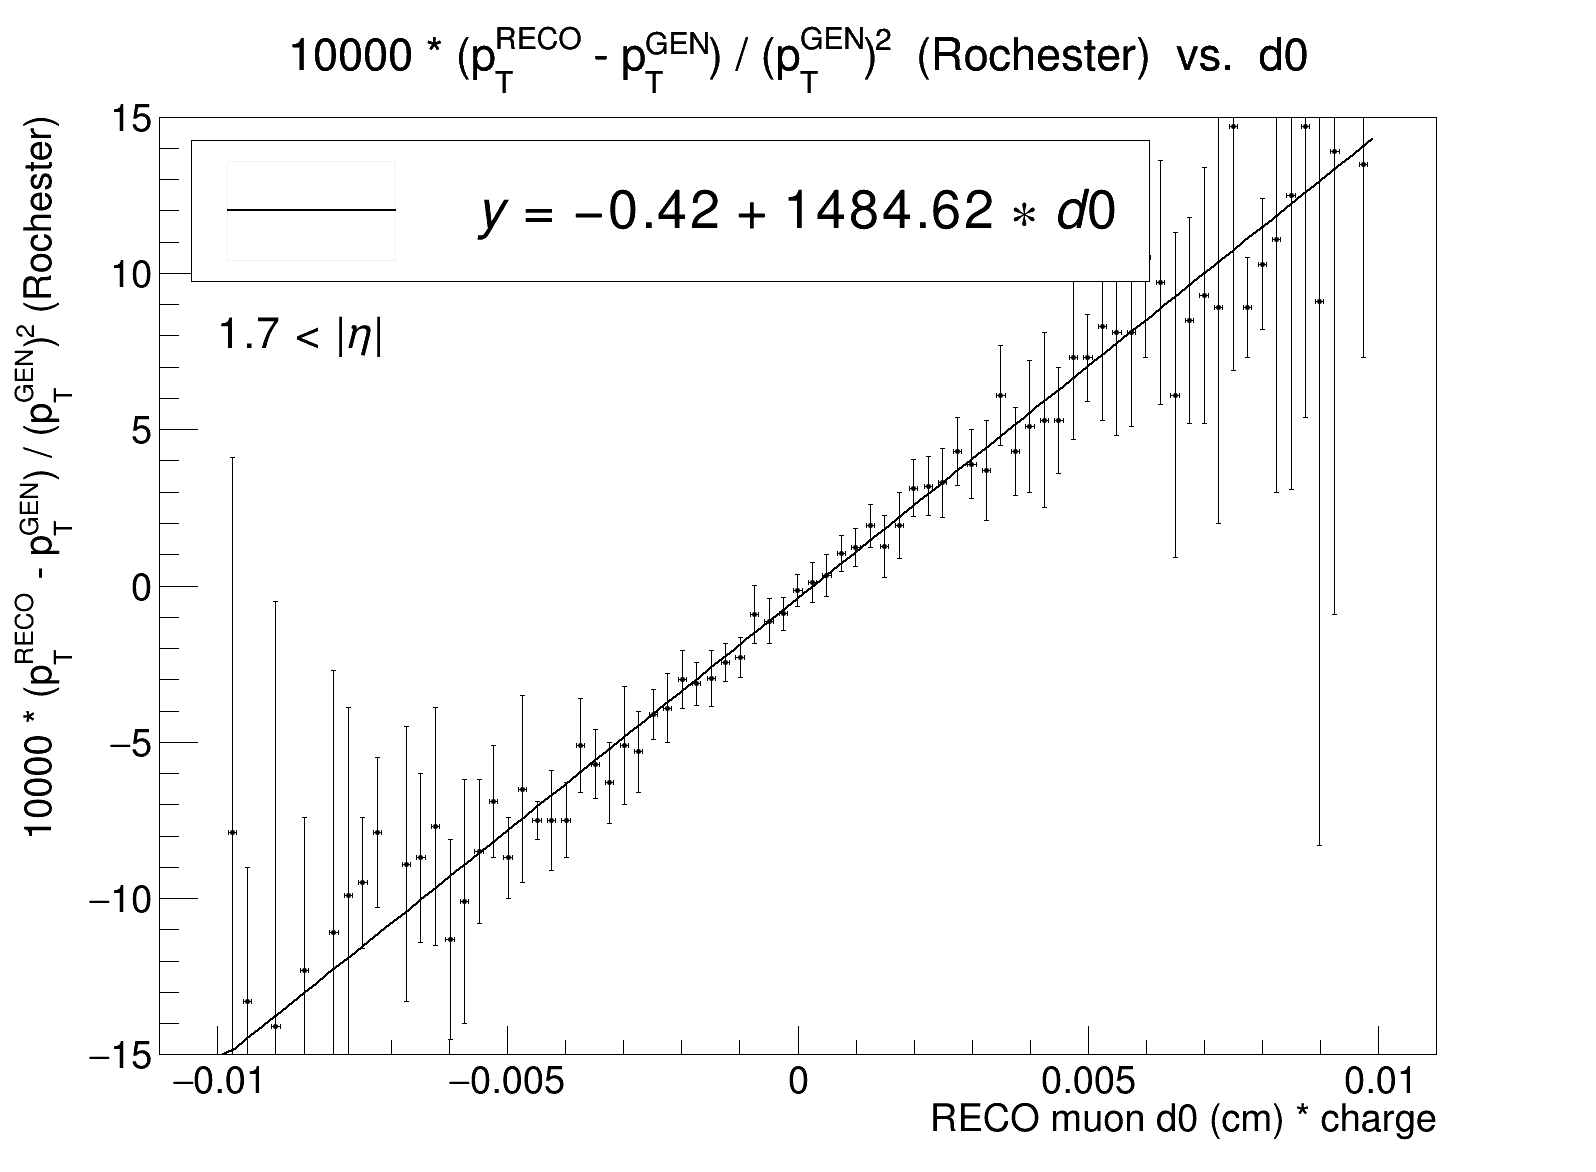
\includegraphics[width=0.32\textwidth]{pics/muon_corr/GeoFit/fit_results/2018_DY_eta_1p7_inf_dRelPt2p0_Roch.png}
      \caption{Plots for the $(\pt^{reco}-\pt^{gen})/ (\pt^{gen})^{2}$ vs $d_0$ correlation in the 2018 \DY simulation, 
               and the linear fits to them. Muon tracks are divided into three different |\eta| regions:
               $|\eta| <$ 0.9 (left), 0.9 $< |\eta| <$ 1.7 (middle), and 1.7 $< |\eta|$ (right).
               Plots credit to Efe Yigitbasi.}
      \label{fig:geofit_param_2018}
\end{figure*}

These fit results are applied as the analytic correction to muon \pt, 
based on the $d_0$, \pt, |\eta|, and charge of the muon.
The correction is applied to all muons in data and simulation in all categories in the \hmm analysis, 
unless the muon is tagged for \FSR.
The performance of this correction is detailed in Section~\ref{sec:perf_geofit}.

\subsection{Performance and Validation}\label{sec:perf_geofit}

The \GeoFit removes the \pt dependence on $d_0$, 
whose overall effect on the \zmm peak is illustrated in Figure~\ref{fig:mucal_d0_run2}.
A clear trend in the \mmm is seen regarding $d_0$ before the \GeoFit, 
while no significant dependence remains after the correction.
As a side remark, the \mmm mismeasurement in Figure~\ref{fig:mucal_d0_run2} can be as large as 1.5 \GeV for extreme $d_0$ values,
but in data and simulation the distribution of the muon $d_0$ is roughly a Gaussian shape with a standard deviation around 15 \mum.
So most of the events are near the center of the plots, and the size of the correction is not as exaggerated as the values at the tails. 

\begin{figure*}[!htb]
      \centering
%      \captionsetup{justification=justified}
      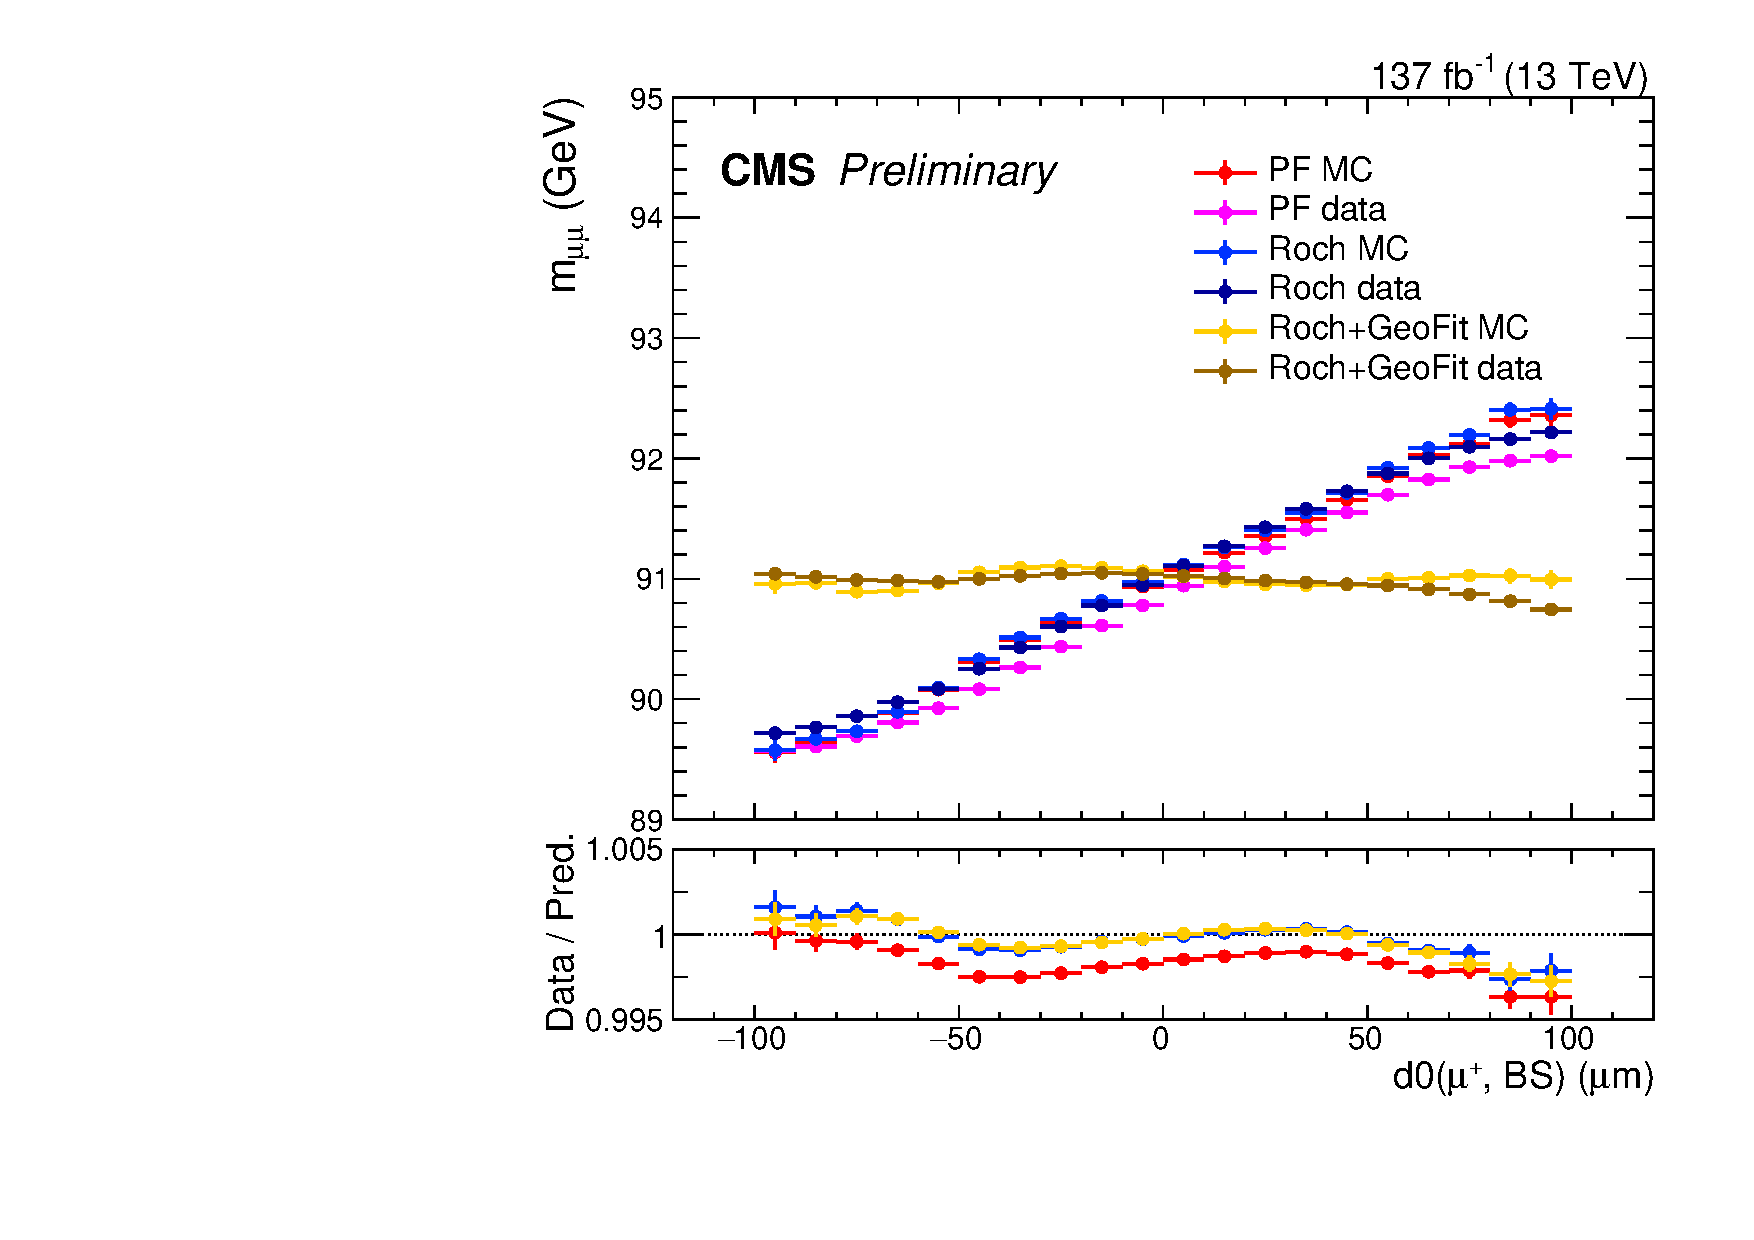
\includegraphics[width=0.45\textwidth]{pics/muon_corr/GeoFit/performance/muP_d0_summary_mean.pdf}
      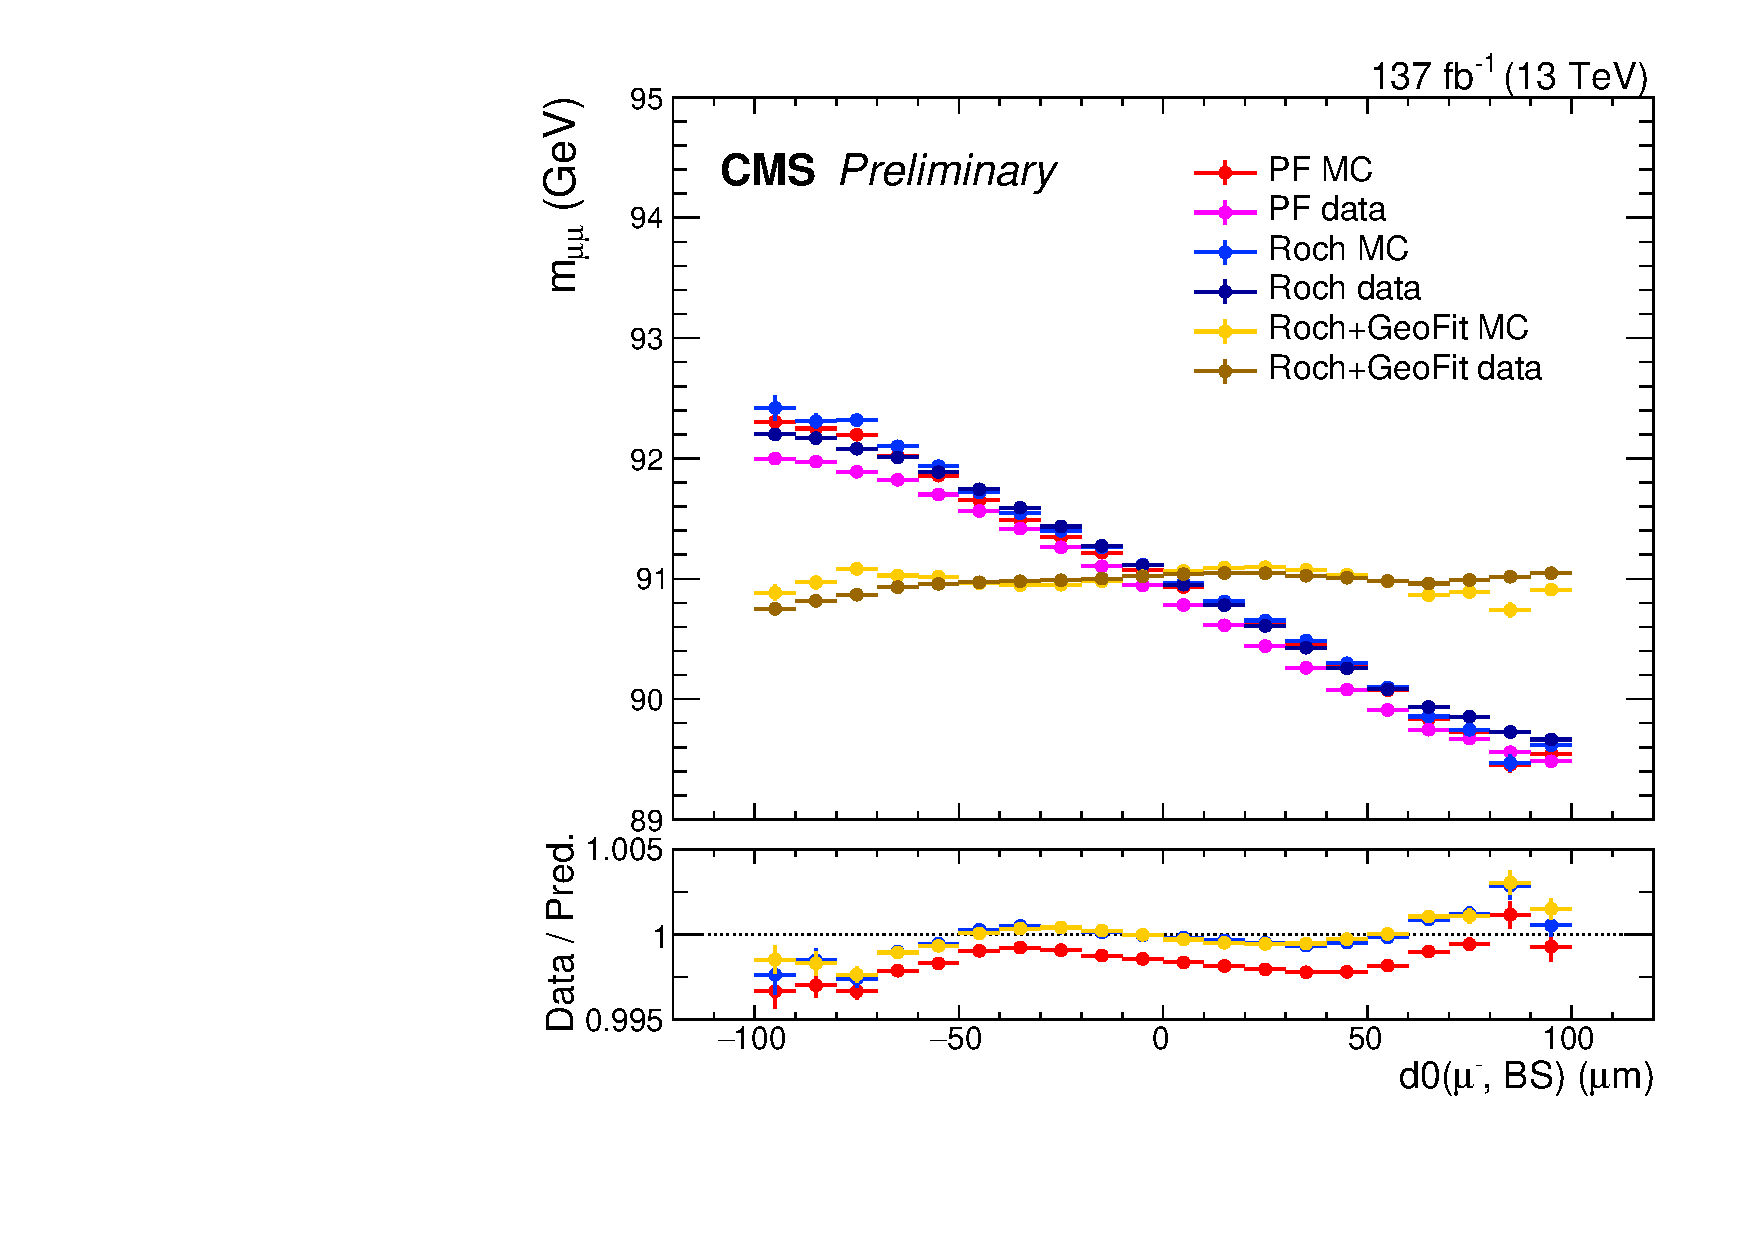
\includegraphics[width=0.45\textwidth]{pics/muon_corr/GeoFit/performance/muN_d0_summary_mean.pdf}
      \caption{Plots showing the \pt dependence on the $d_0$ value with different stages of muon correction.
               The plots compare the \zmm peak in data and simulation for three years (2016-2018) combined.
               All positively charged muons are put in the left plot and all negatively charged ones are put in the right plot.
               The $\pt-d_0$ dependence is reversed for positive and negative muons.
               }
      \label{fig:mucal_d0_run2}
\end{figure*}


\begin{figure*}[!htb]
      \centering
%      \captionsetup{justification=justified}
      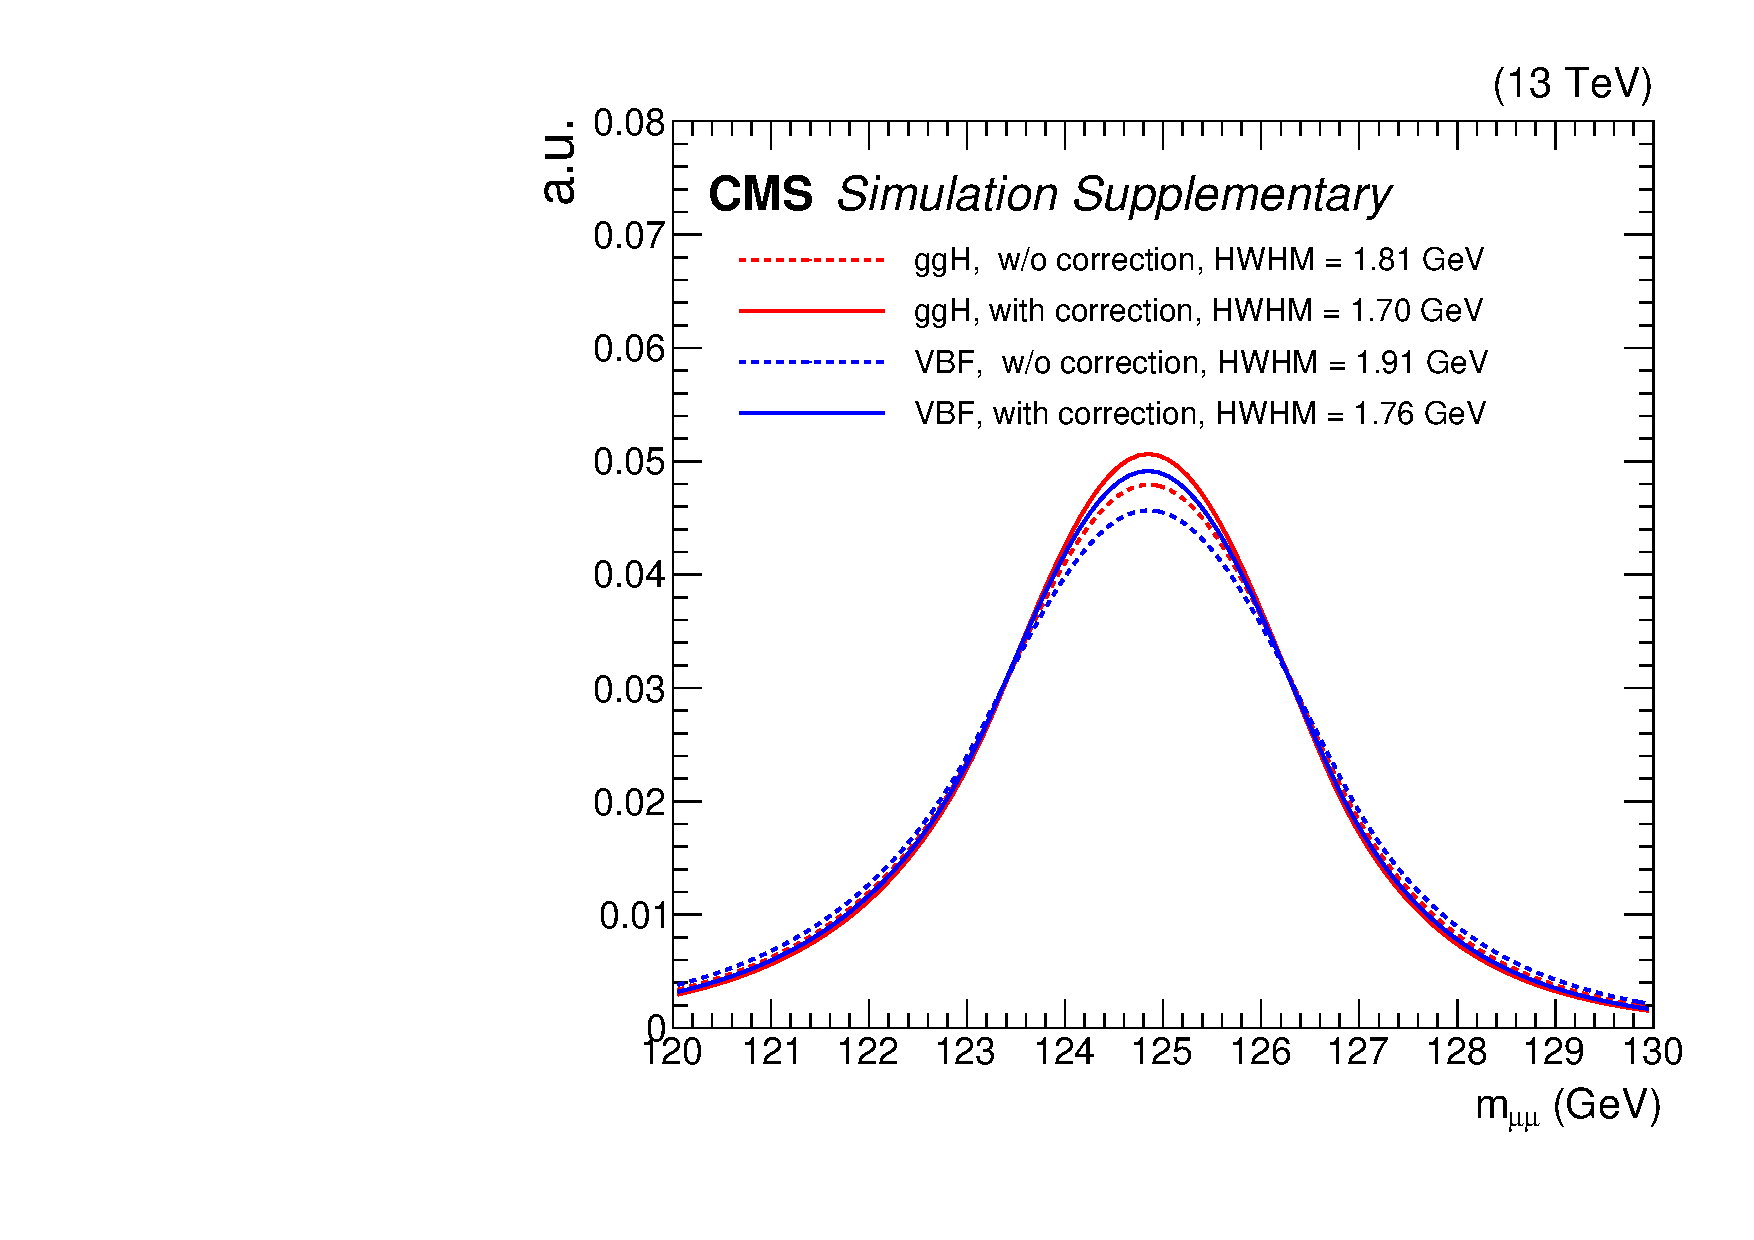
\includegraphics[width=0.45\textwidth]{pics/muon_corr/GeoFit/performance/ggHVBF.pdf}
      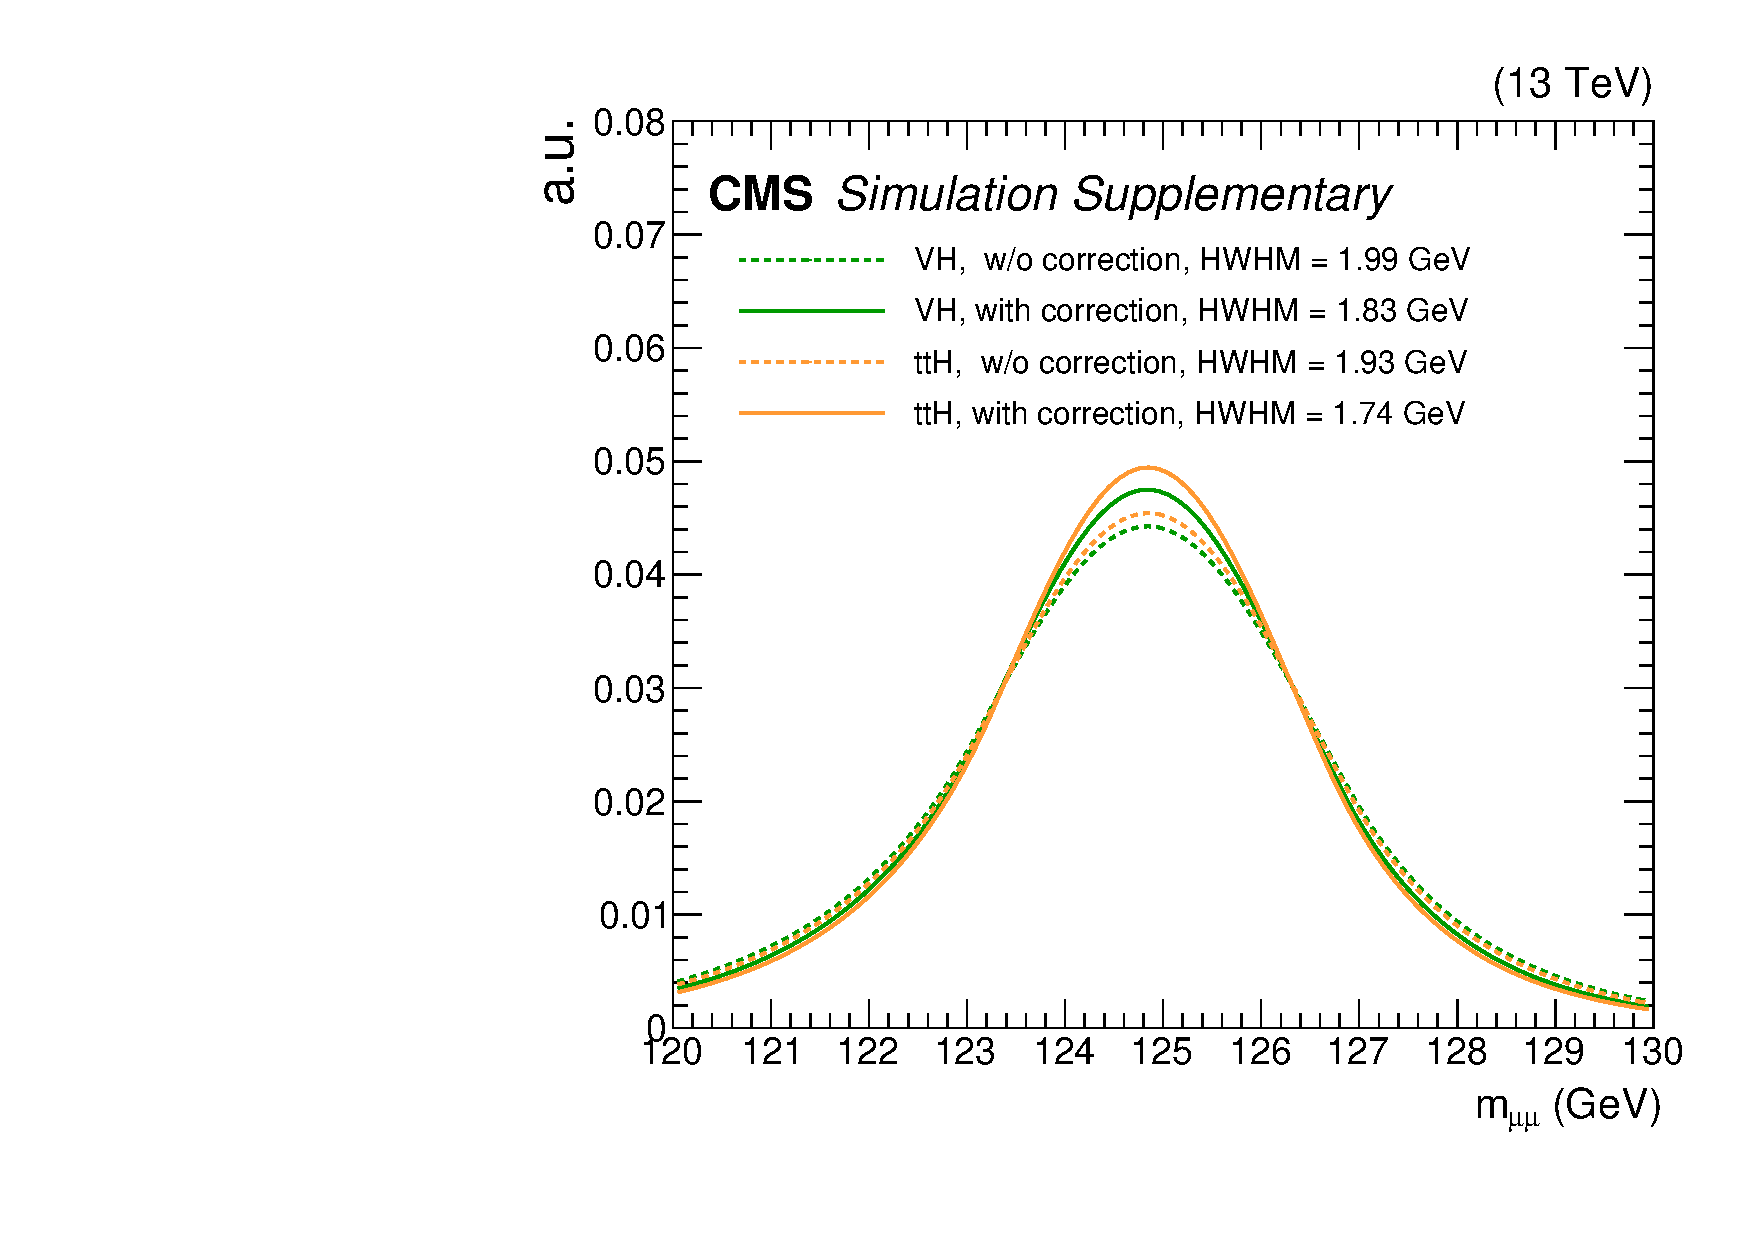
\includegraphics[width=0.45\textwidth]{pics/muon_corr/GeoFit/performance/VHttH.pdf}
      \caption{Plots showing the \GeoFit improvement on the four main \hmm signal modes, 
               \ggH and \qqH plotted on the left, and \VH and \ttH plotted on the right.
               The plots are made combining the expected signal in all three years of data-taking (2016-2018).
               The relative improvements on \mmm resolution for \ggH, \qqH, \VH, and \ttH modes are, respectively,
               6.1\%, 7.8\%, 8.0\%, and 9.8\%.
               }
      \label{fig:geofit_sigs}
\end{figure*}

Overall, the removal of the $\pt-d_0$ dependence leads to an improvement on the inclusive \mmm resolution.
This improvement is different for different processes depending on their kinematic profiles in \pt and |\eta|.
Figure~\ref{fig:geofit_sigs} shows the improvement on \mmm resolution in the four main expected signal modes, \ggH, \qqH, \VH, and \ttH.
The relative improvements on \mmm resolution for \ggH, \qqH, \VH, and \ttH modes are, 
respectively, 6.1\%, 7.8\%, 8.0\%, and 9.8\%.
This improvement on signal resolution translates to about 5\% improvement on the significance of the inclusive \hmm analysis.

The different improvements in different signal modes comes from their \pt profiles.
As the correction is proportional to $d_0$ and $\pt^{2}$, 
the relative improvement $\Delta\pt / \pt$ is proportional to $d_0$ and \pt. 
Figure~\ref{fig:sigs_d0_pt} shows the $d_0$ (left) and \pt (right) distributions of different signal modes.
The $d_0$ profiles of the 4 signals are exactly the same,
while the \pt profiles are different.
\ttH signal has more high \pt muons than other signal modes,
while \ggH signal has more muons on the low \pt side.
Therefore they gain the largest and smallest improvements from the \GeoFit, respectively.
\qqH and \VH signals have very similar \pt profiles, 
and their improvements from the \GeoFit are about the same.

\begin{figure*}[!htb]
      \centering
%      \captionsetup{justification=justified}
      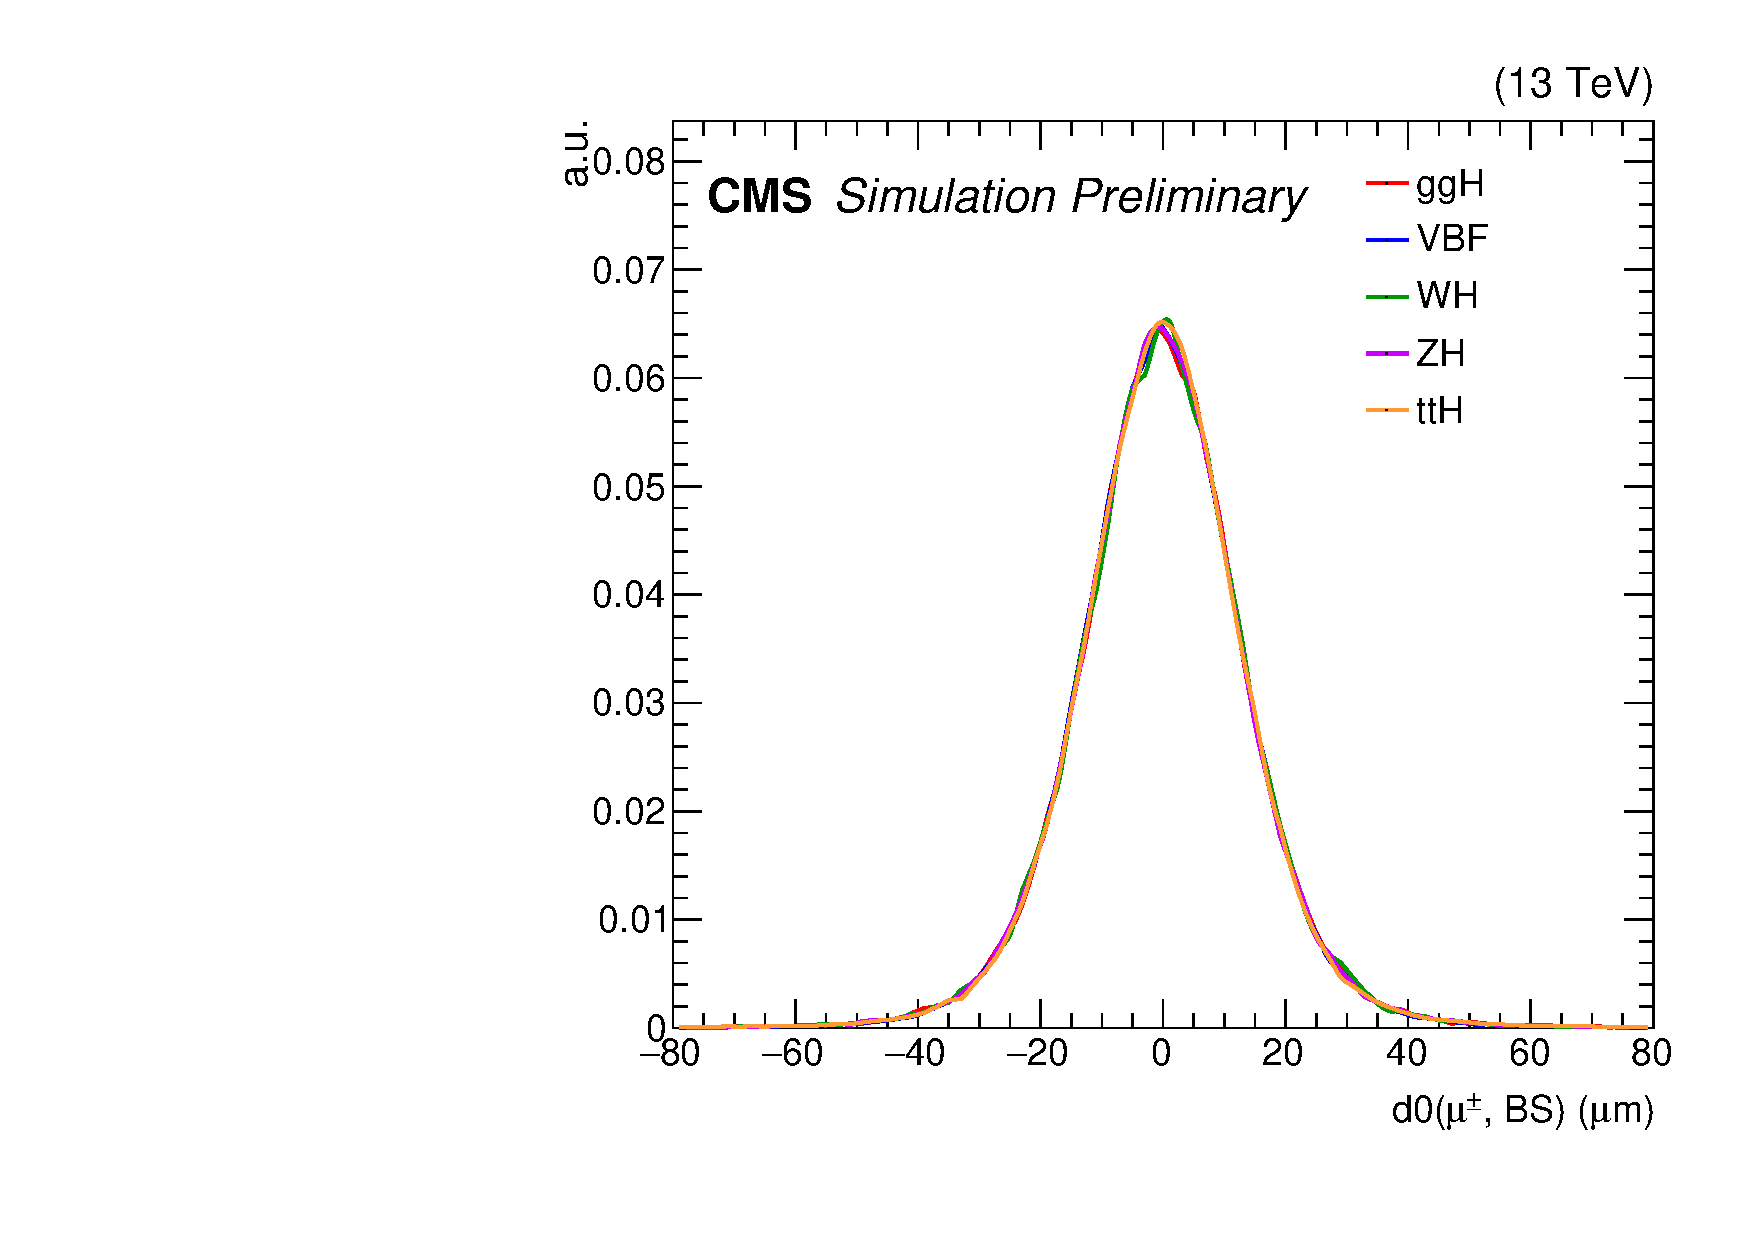
\includegraphics[width=0.45\textwidth]{pics/muon_corr/GeoFit/performance/samp_d0.pdf}
      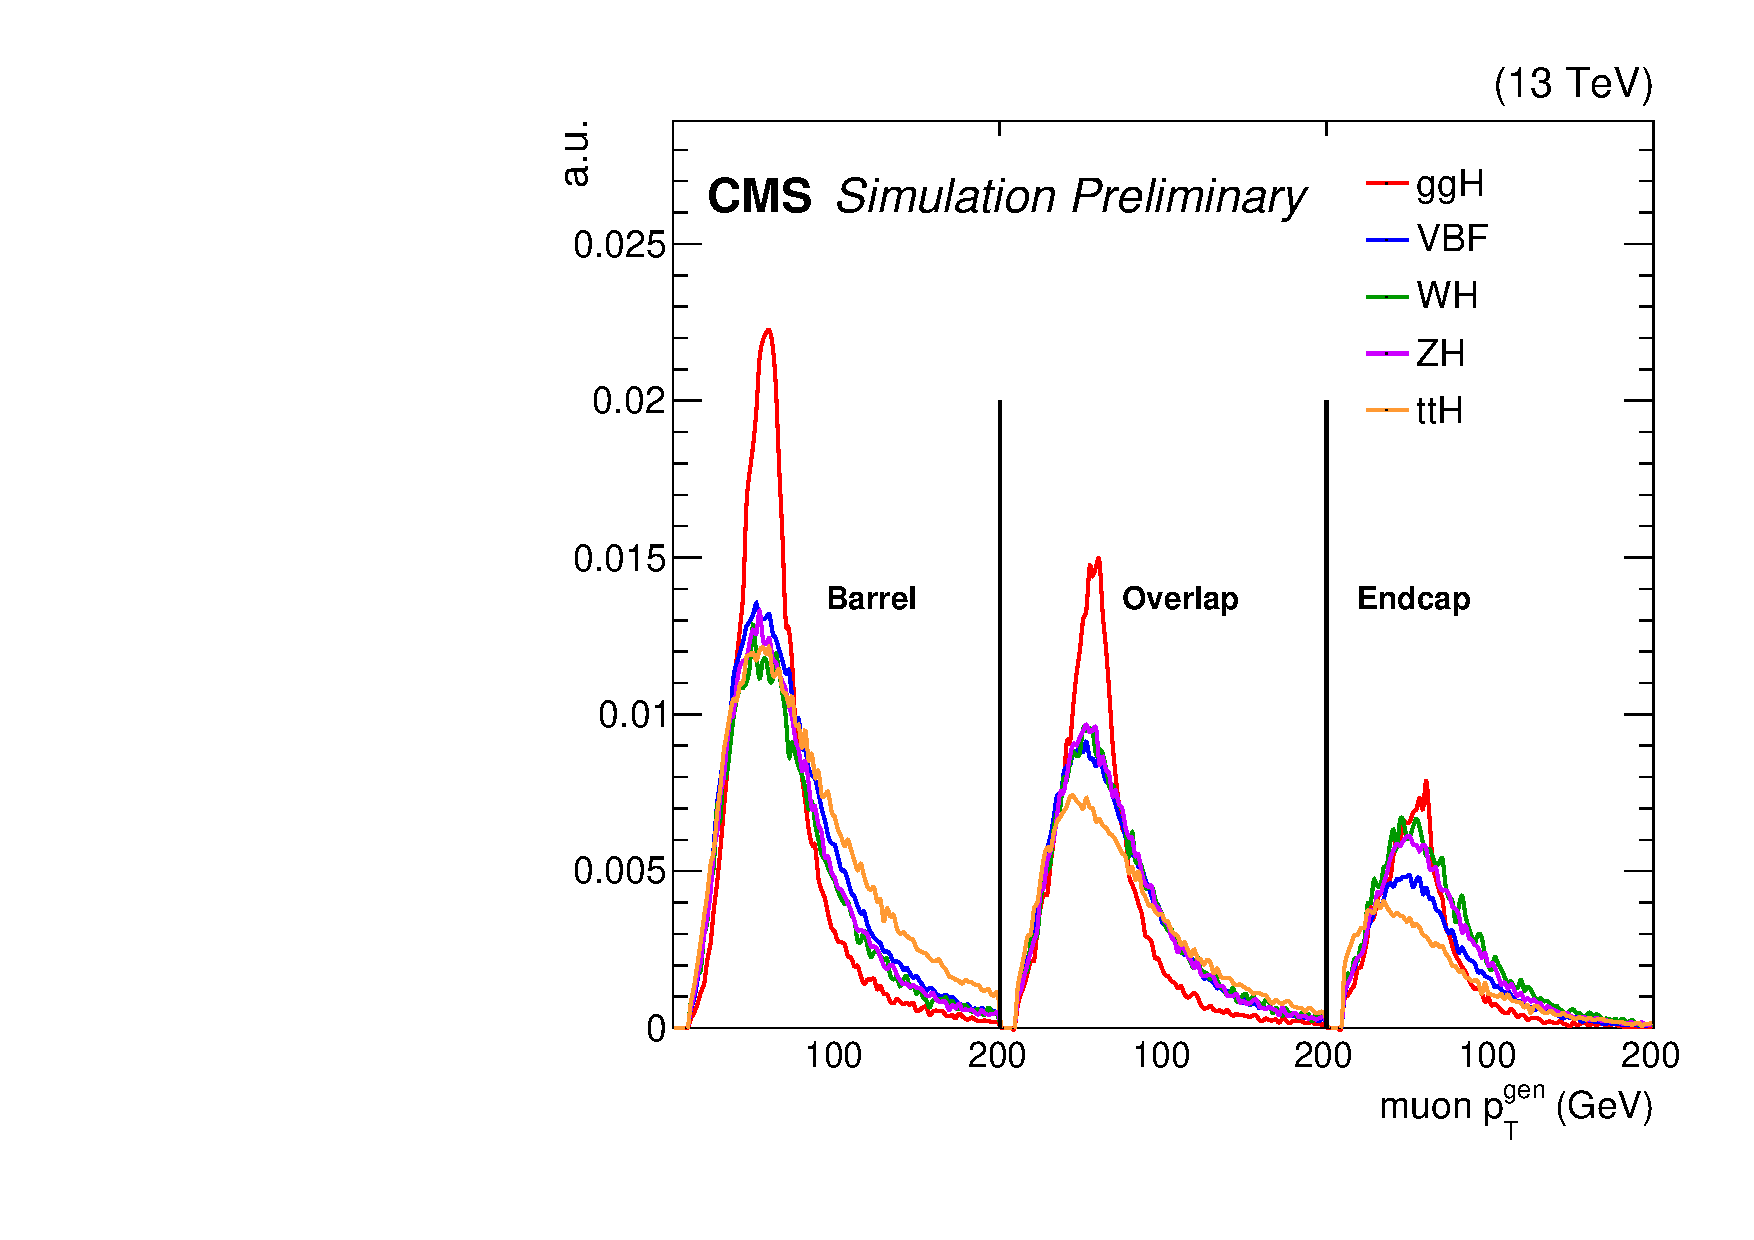
\includegraphics[width=0.45\textwidth]{pics/muon_corr/GeoFit/performance/samp_pt_BOE.pdf}
      \caption{Plots showing $d_0$ and \pt distributions of the four main \hmm signal modes. 
               The $d_0$ profiles (left plot) of the 4 signals are the same.
               The \pt profiles (right plot) are different, which explains the different relative improvements  
               that the signals receive from the \GeoFit.
               }
      \label{fig:sigs_d0_pt}
\end{figure*}



\subsection{GeoFit vs Track Refit}\label{sec:track_refit}

The \GeoFit provides a simple method to correct the \pt dependence on d0 based on high level physics variables.
Since the origin of this \pt dependence is well-understood, it is also possible to derive a more fundamental correction
by refitting each muon track including the BS position as an additional constraint to the track.
This method requires lower-level information of muon reconstruction and is computationally more expensive,
but is in principle more precise.
To compare the performance of the \GeoFit and the refit method, a preliminary study is made on the 2018 \ggH signal simulation.
The \mmm shape of the inclusive signal is plotted applying the track refit method vs applying the \GeoFit, shown in Figure~\ref{fig:refit_vs_geofit}.
This comparison shows that the \mmm shapes from the two methods are almost equivalent.
The \GeoFit, although an approximation method, captures most of the effect and provides about the same improvement in \mmm resolution as the refit method.
The \GeoFit is therefore chosen in the \hmm analysis to speed up the workflow.

\begin{figure*}[!htb]
      \centering
%      \captionsetup{justification=justified}
      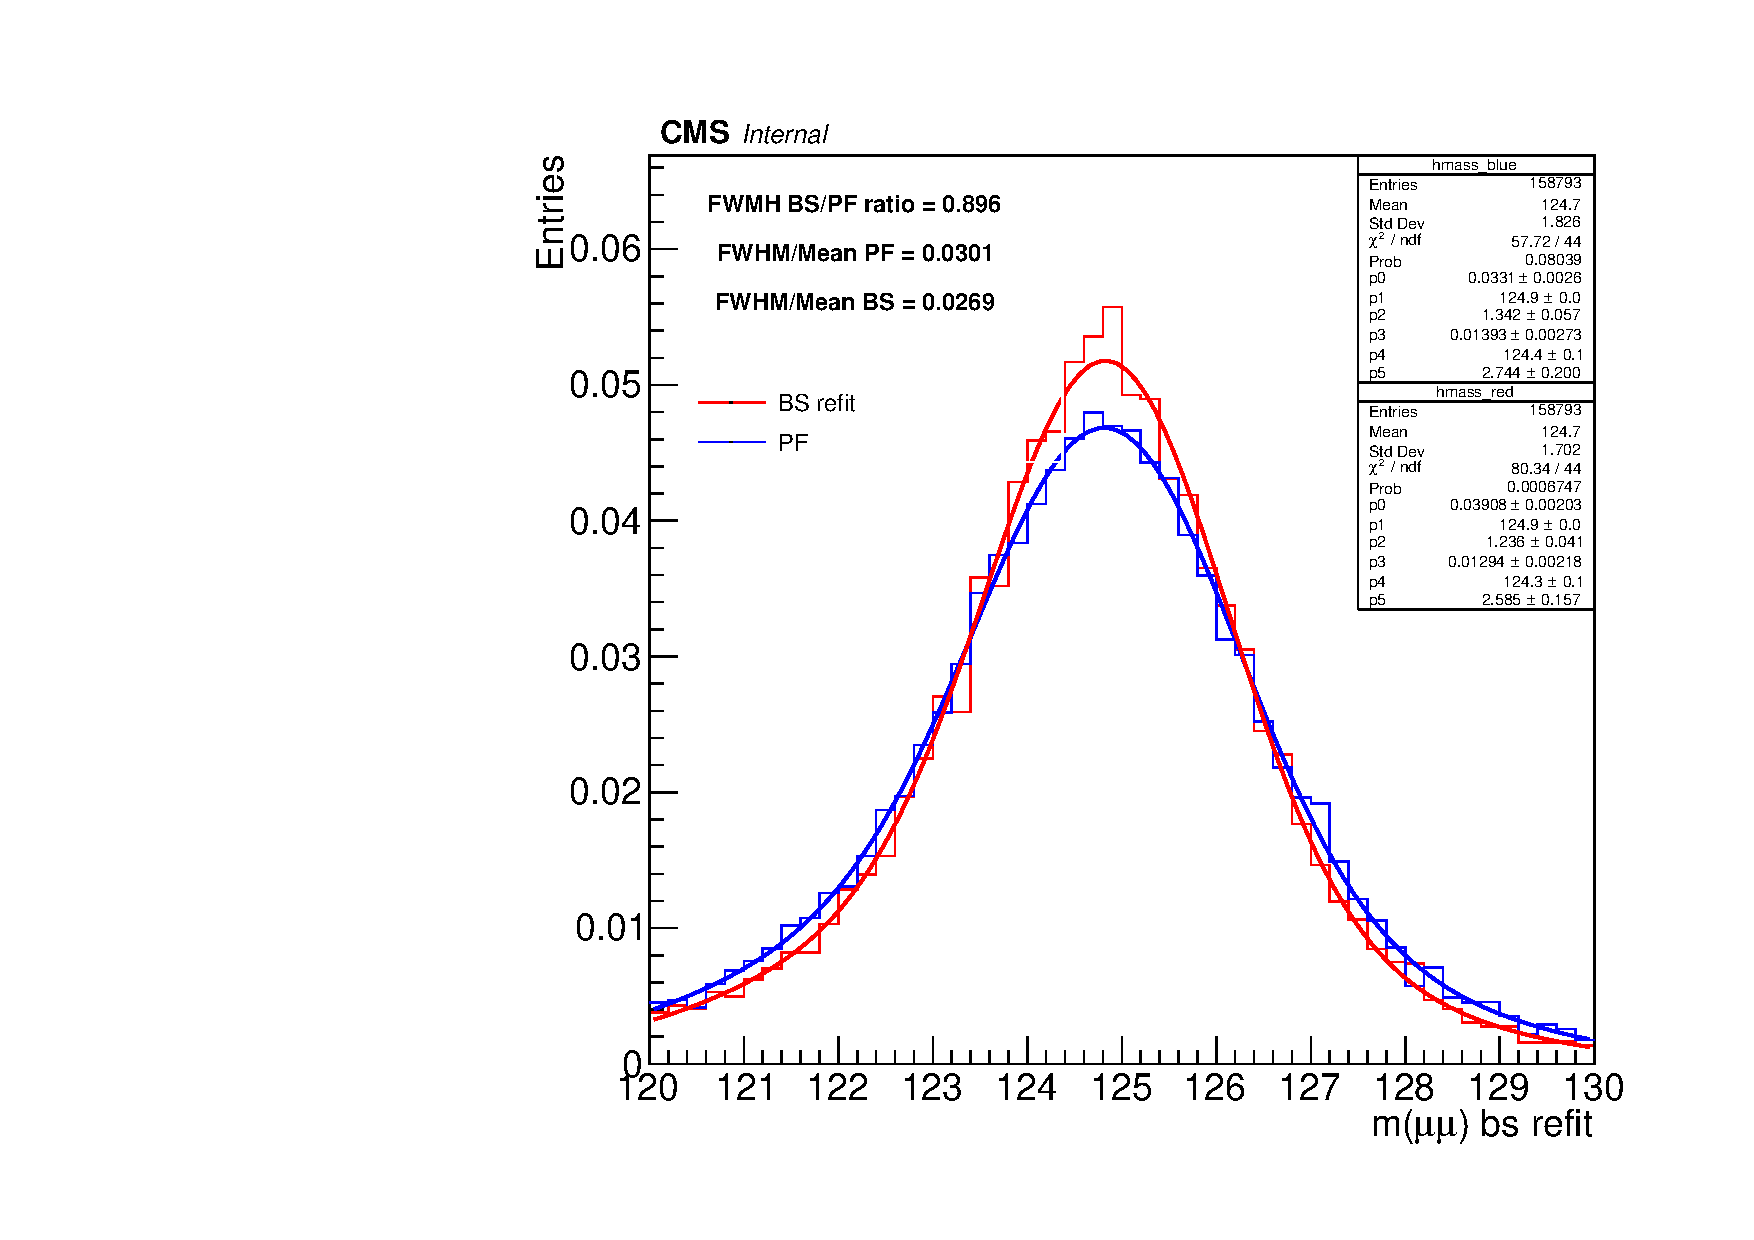
\includegraphics[width=0.45\textwidth]{pics/muon_corr/GeoFit/track_refit/ggH_mass_muon_fit_bs_pf_2018.pdf}
      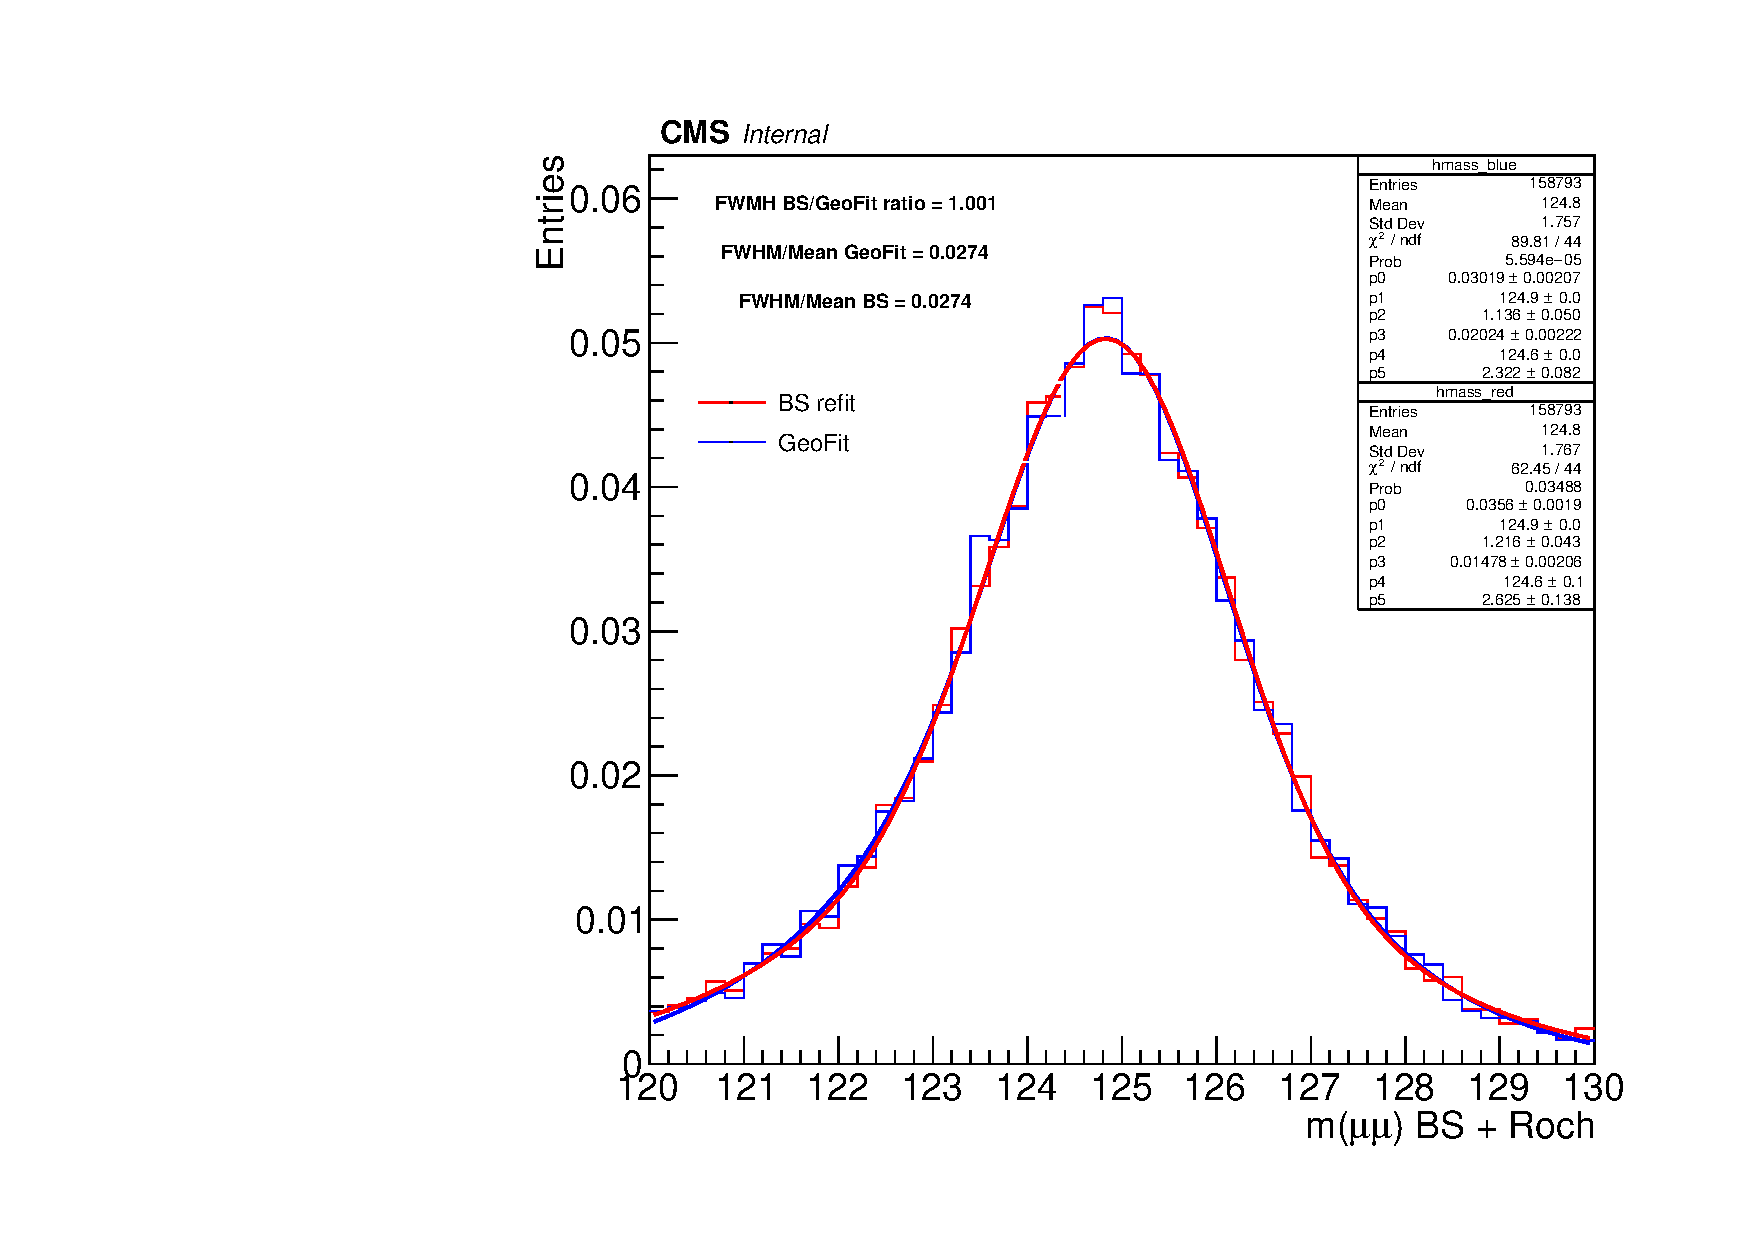
\includegraphics[width=0.45\textwidth]{pics/muon_corr/GeoFit/track_refit/ggH_mass_muon_fit_bs_geofit_2018.pdf}
      \caption{Plots of the \mmm shape of the 2018 \ggH simulation sample, comparing different muon correction methods.
               The left plot shows the \mmm distribution calculated with muon tracks refitted with the additional BS constraint, 
               compared with the particle flow shape (left plot).
               The \RochCorr is not applied in the left plot for both the red and the blue lines.
               The right plot shows the \mmm distribution from the refit method, with the \RochCorr applied,
               compared with the shape from \GeoFit + \RochCorr (right plot).
               Plots credit to Pierluigi Bortignon.}
      \label{fig:refit_vs_geofit}
\end{figure*}

\section{Muon Calibration Results} \label{sec:muon_cal}

The \zmm is a well-understood process with a mass scale not far from the Higgs boson and with a much larger number of events at the LHC.
It is therefore used as a candle to monitor the performance of the \RochCorr and the \GeoFit, 
and validate that these corrections do not introduce new biases.
In this study, the distribution of the \mmm is plotted in different bins of various dimuon kinematic variables.
The \mmm distributions are fit with a Voigtian + Exponential function, 
in which the Voigtian part is a convolution of a Breit-Wigner function and a Gaussian function.
The parameter "mean mass" from the Breit-Wigner part and standard deviation from the Gaussian part are 
taken as the mean value and the experimental resolution of the \mmm distribution.
They are plotted against the dimuon kinematic variable of interest to check for potential trends.

The calibration plots are made by year as the corrections are provided by year.
Events containing \FSR are removed from this study as it is a separate effect.
Different variables are tested in the Figures listed: 
Figure~\ref{fig:mucal_muP_eta} for the \eta ~of the positive muon,
Figure~\ref{fig:mucal_muP_phi} for the \phi ~of the positive muon,
Figure~\ref{fig:mucal_muN_phi} for the \phi ~of the negative muon,
Figure~\ref{fig:mucal_muP_pt} for the \pt ~of the positive muon,
Figure~\ref{fig:mucal_dimu_pt} for the \pt ~of the dimuon system,
Figure~\ref{fig:mucal_dimu_eta} for the \eta ~of the dimuon system,
Figure~\ref{fig:mucal_muP_d0} for the $d_0$ of the positive muon,
and Figure~\ref{fig:mucal_muN_d0} for the $d_0$ of the negative muon.

From these plots, it can be concluded that all the known biases in muon \pt are removed and no new bias has been introduced.
The \RochCorr and \GeoFit correct orthogonal effects, and do not interfere with the performance of each other.
After the corrections, a per-mille level agreement is achieved between data and simulation in the \mmm value,
while the agreement in \mmm resolution is about a few percent. 

\begin{figure*}[!htb]
      \centering
%      \captionsetup{justification=justified}
      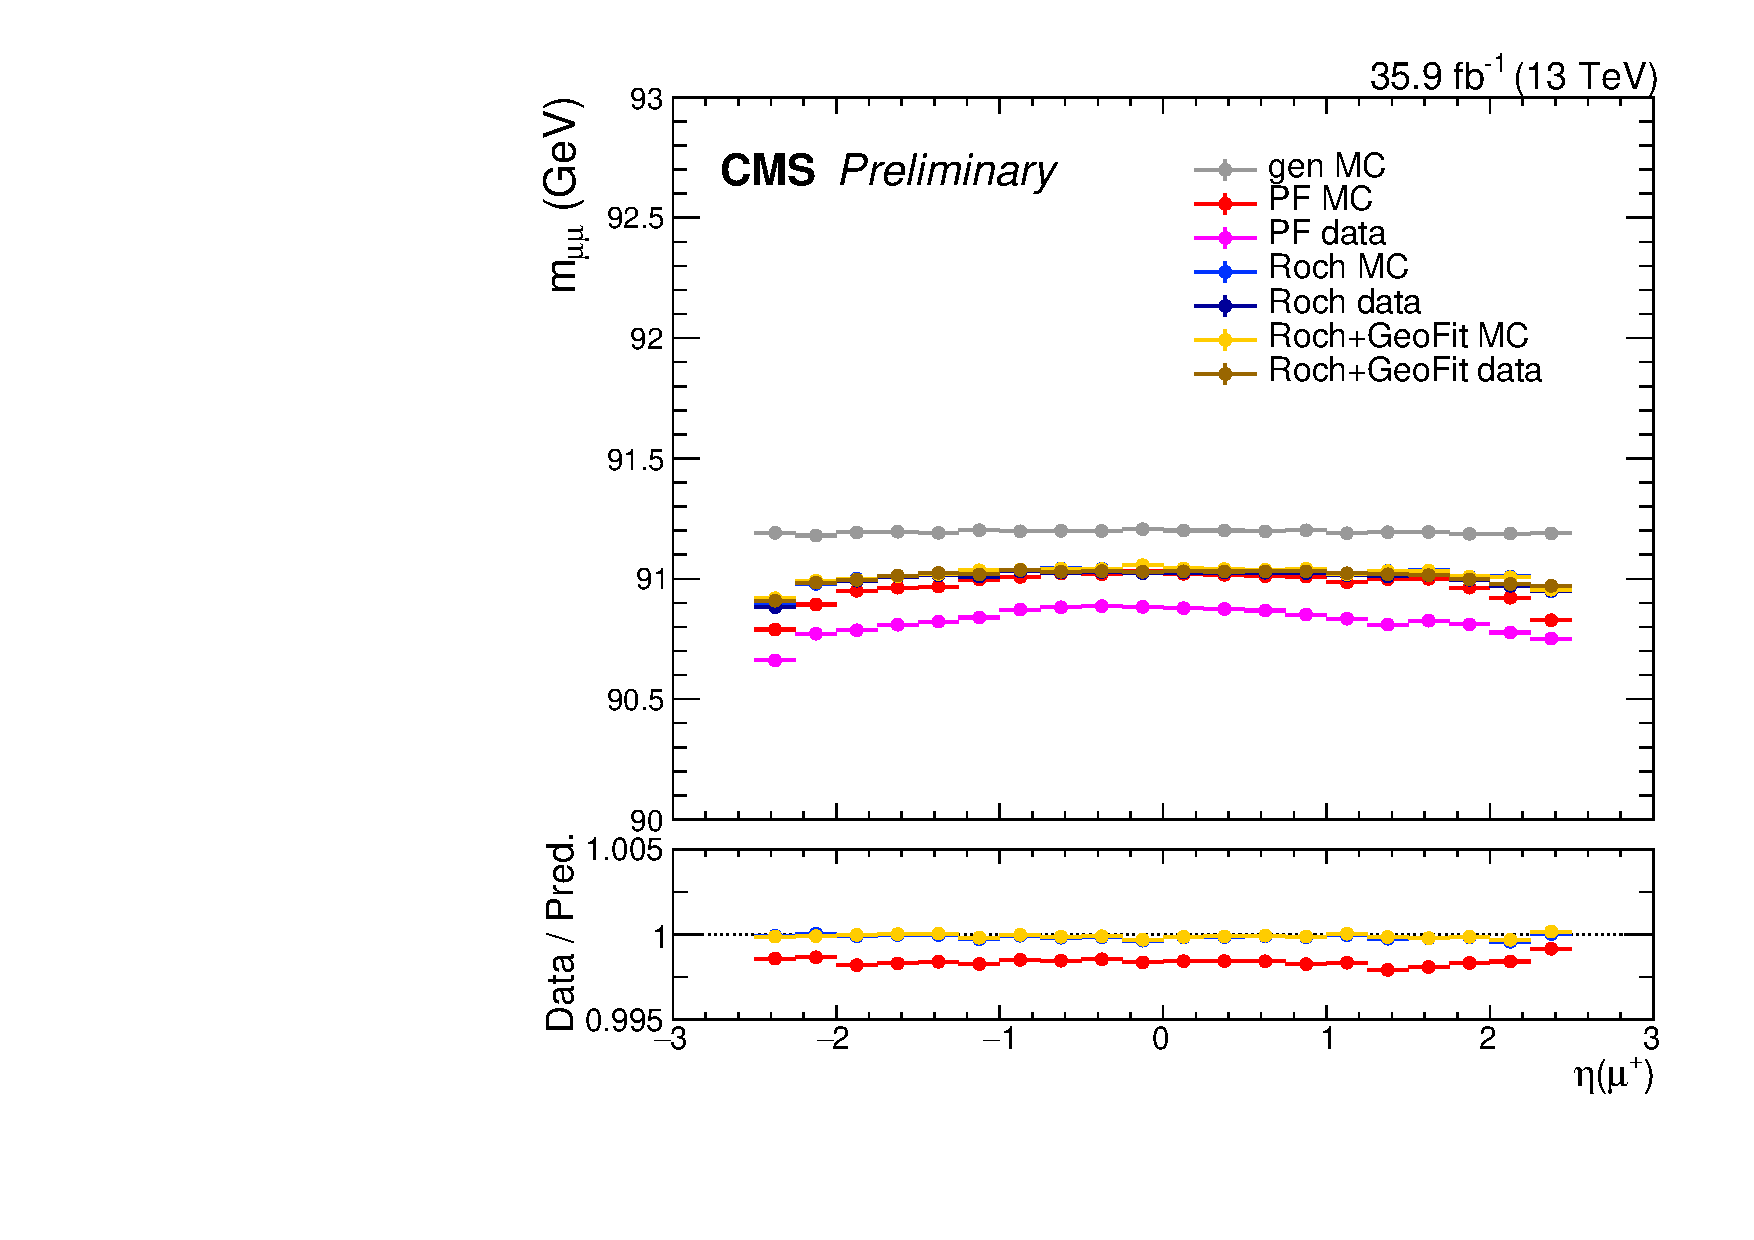
\includegraphics[width=0.32\textwidth]{pics/muon_corr/muon_cal/2016/muP_eta_summary_mean.pdf}
      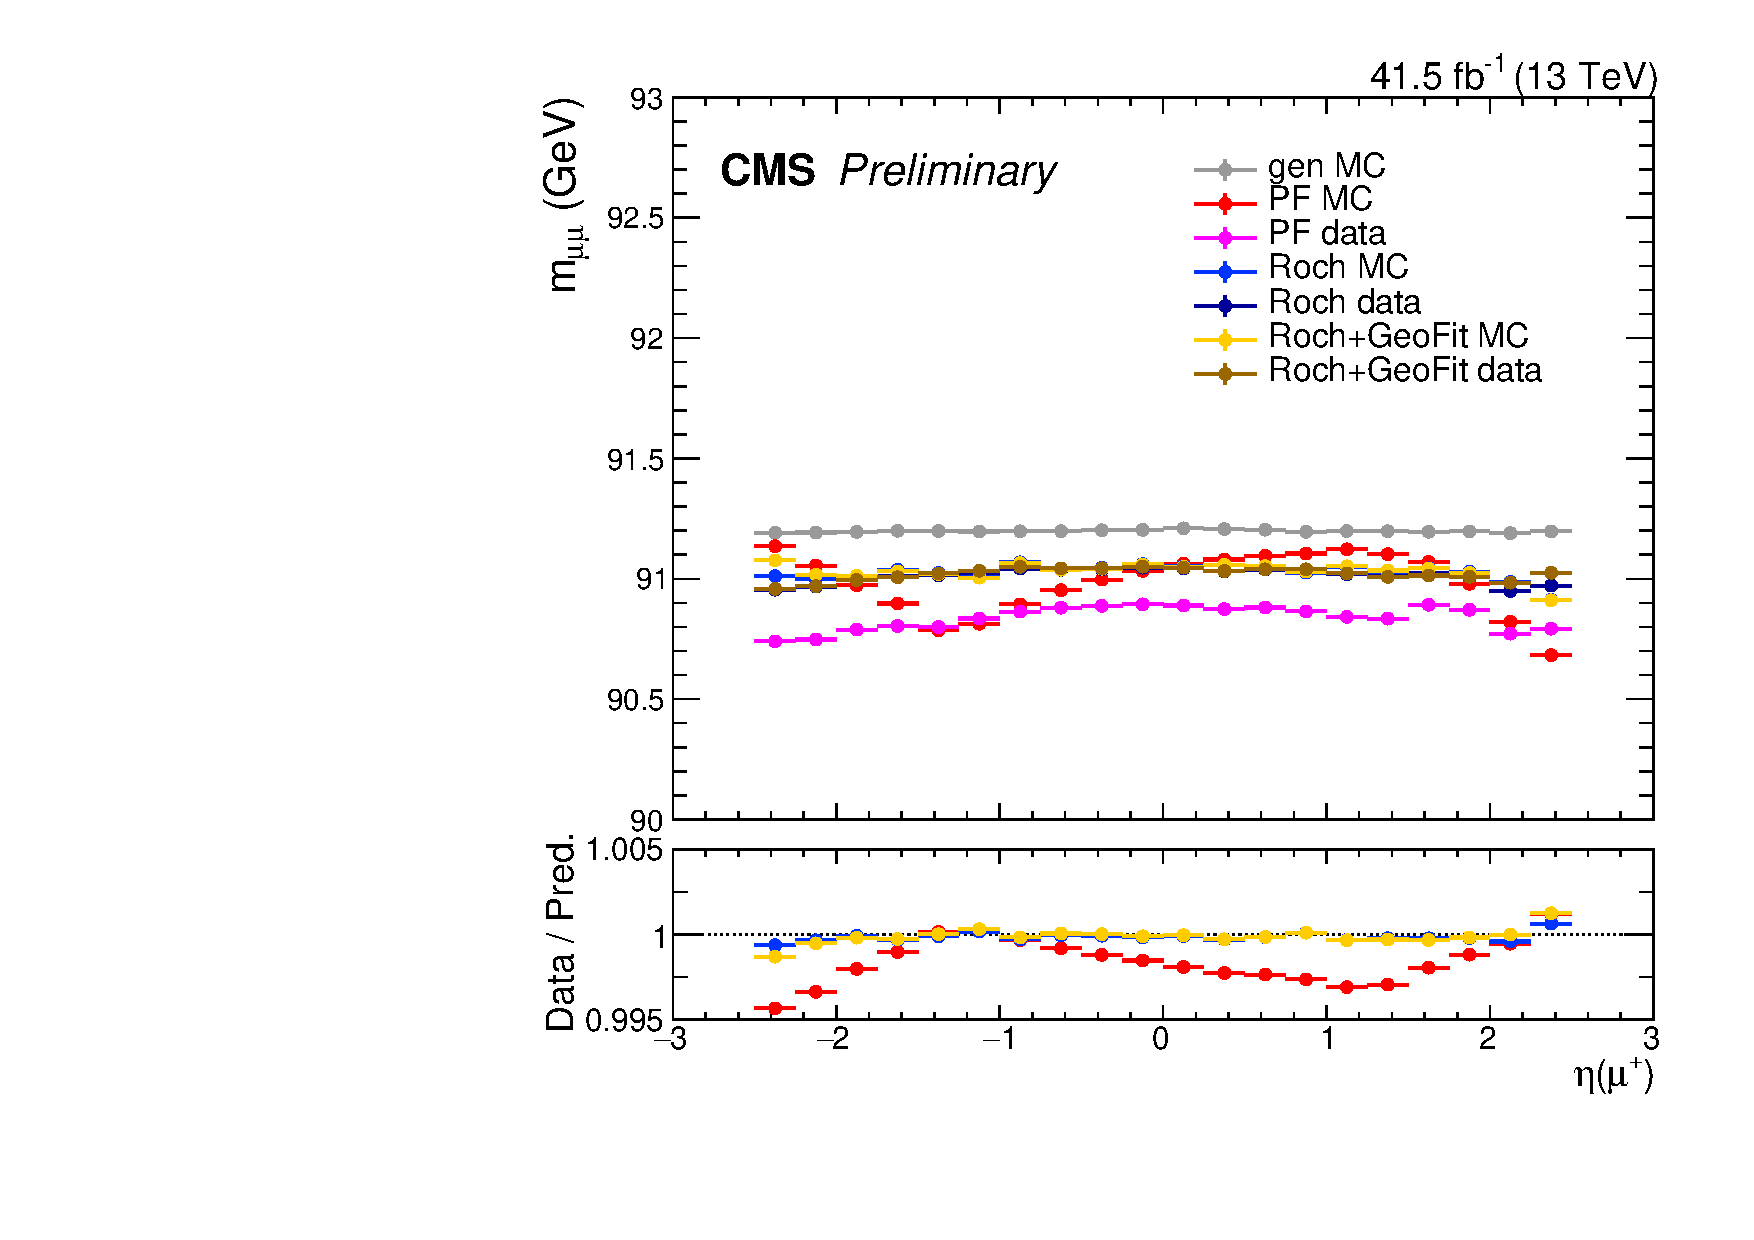
\includegraphics[width=0.32\textwidth]{pics/muon_corr/muon_cal/2017/muP_eta_summary_mean.pdf}
      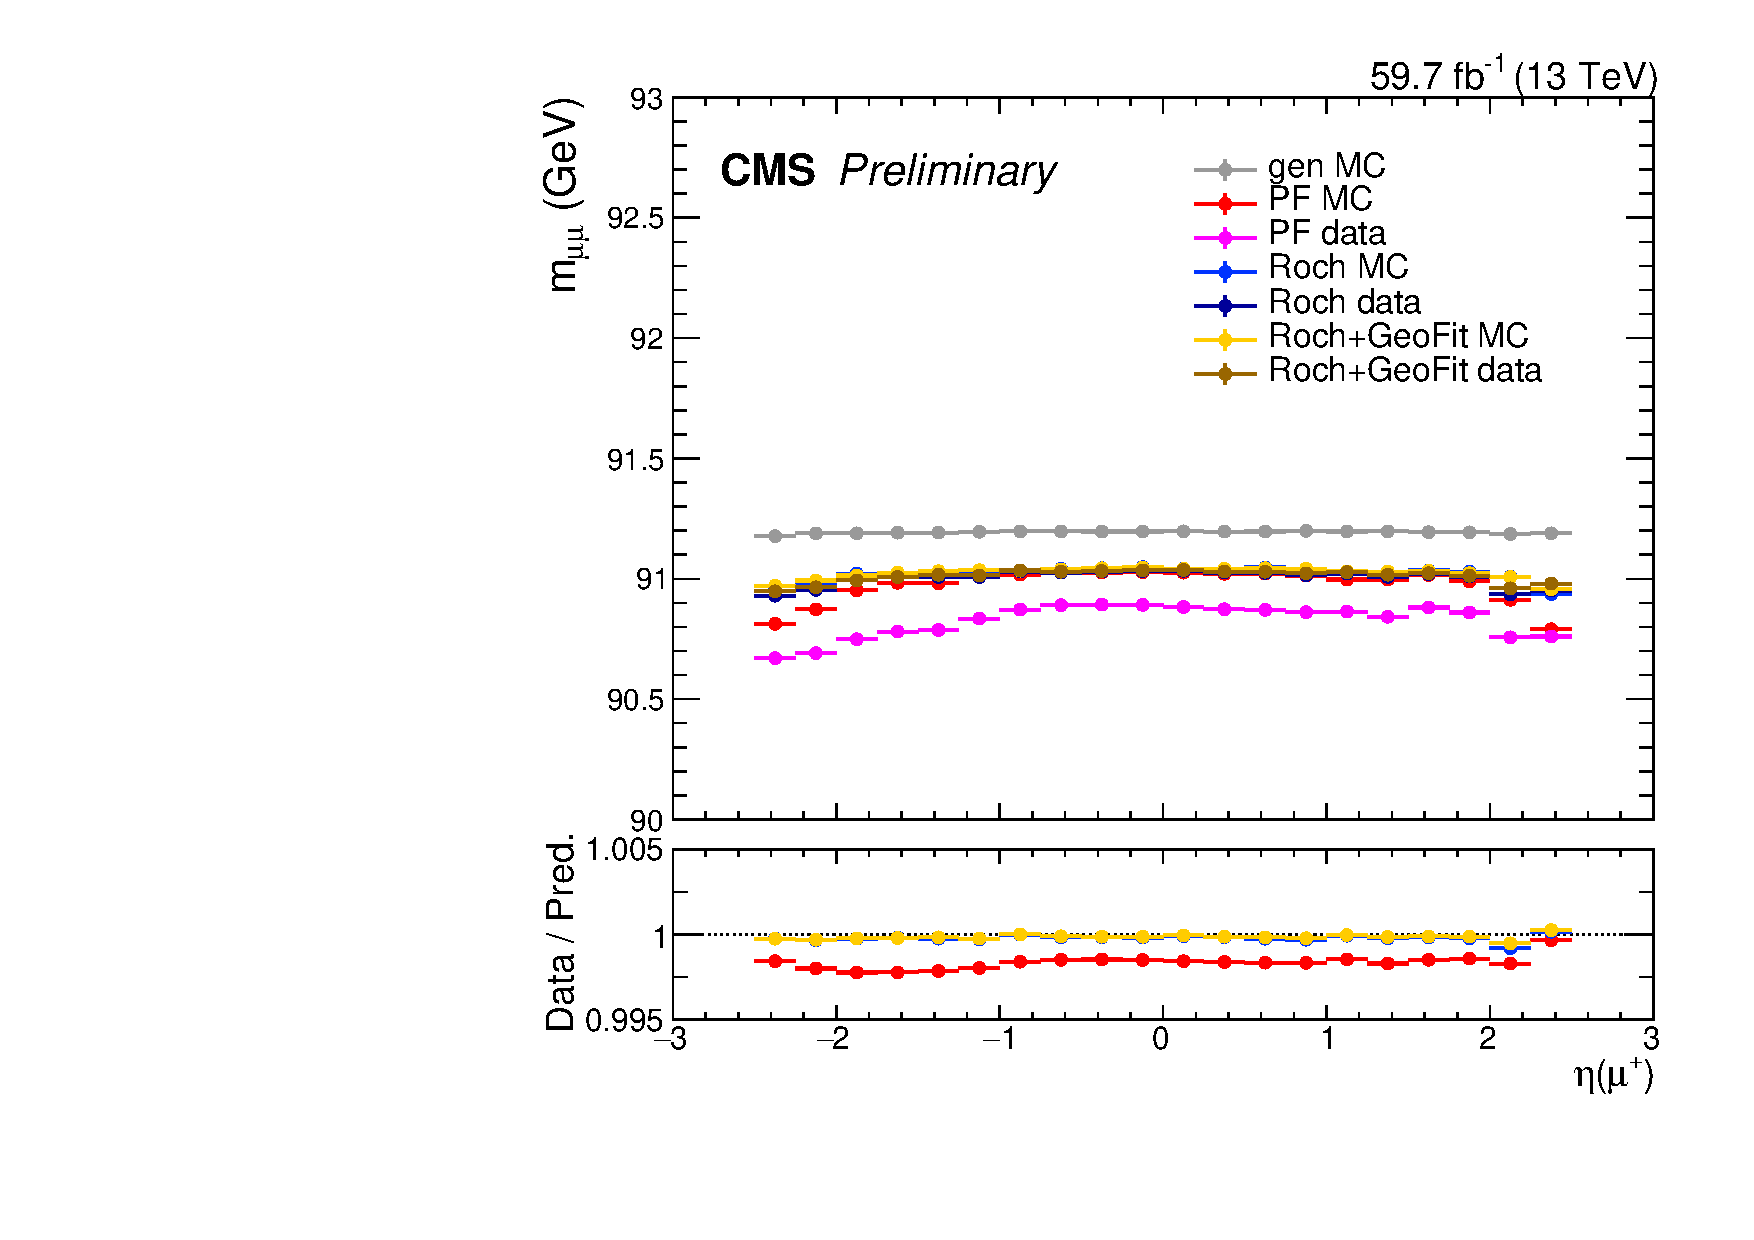
\includegraphics[width=0.32\textwidth]{pics/muon_corr/muon_cal/2018/muP_eta_summary_mean.pdf}
      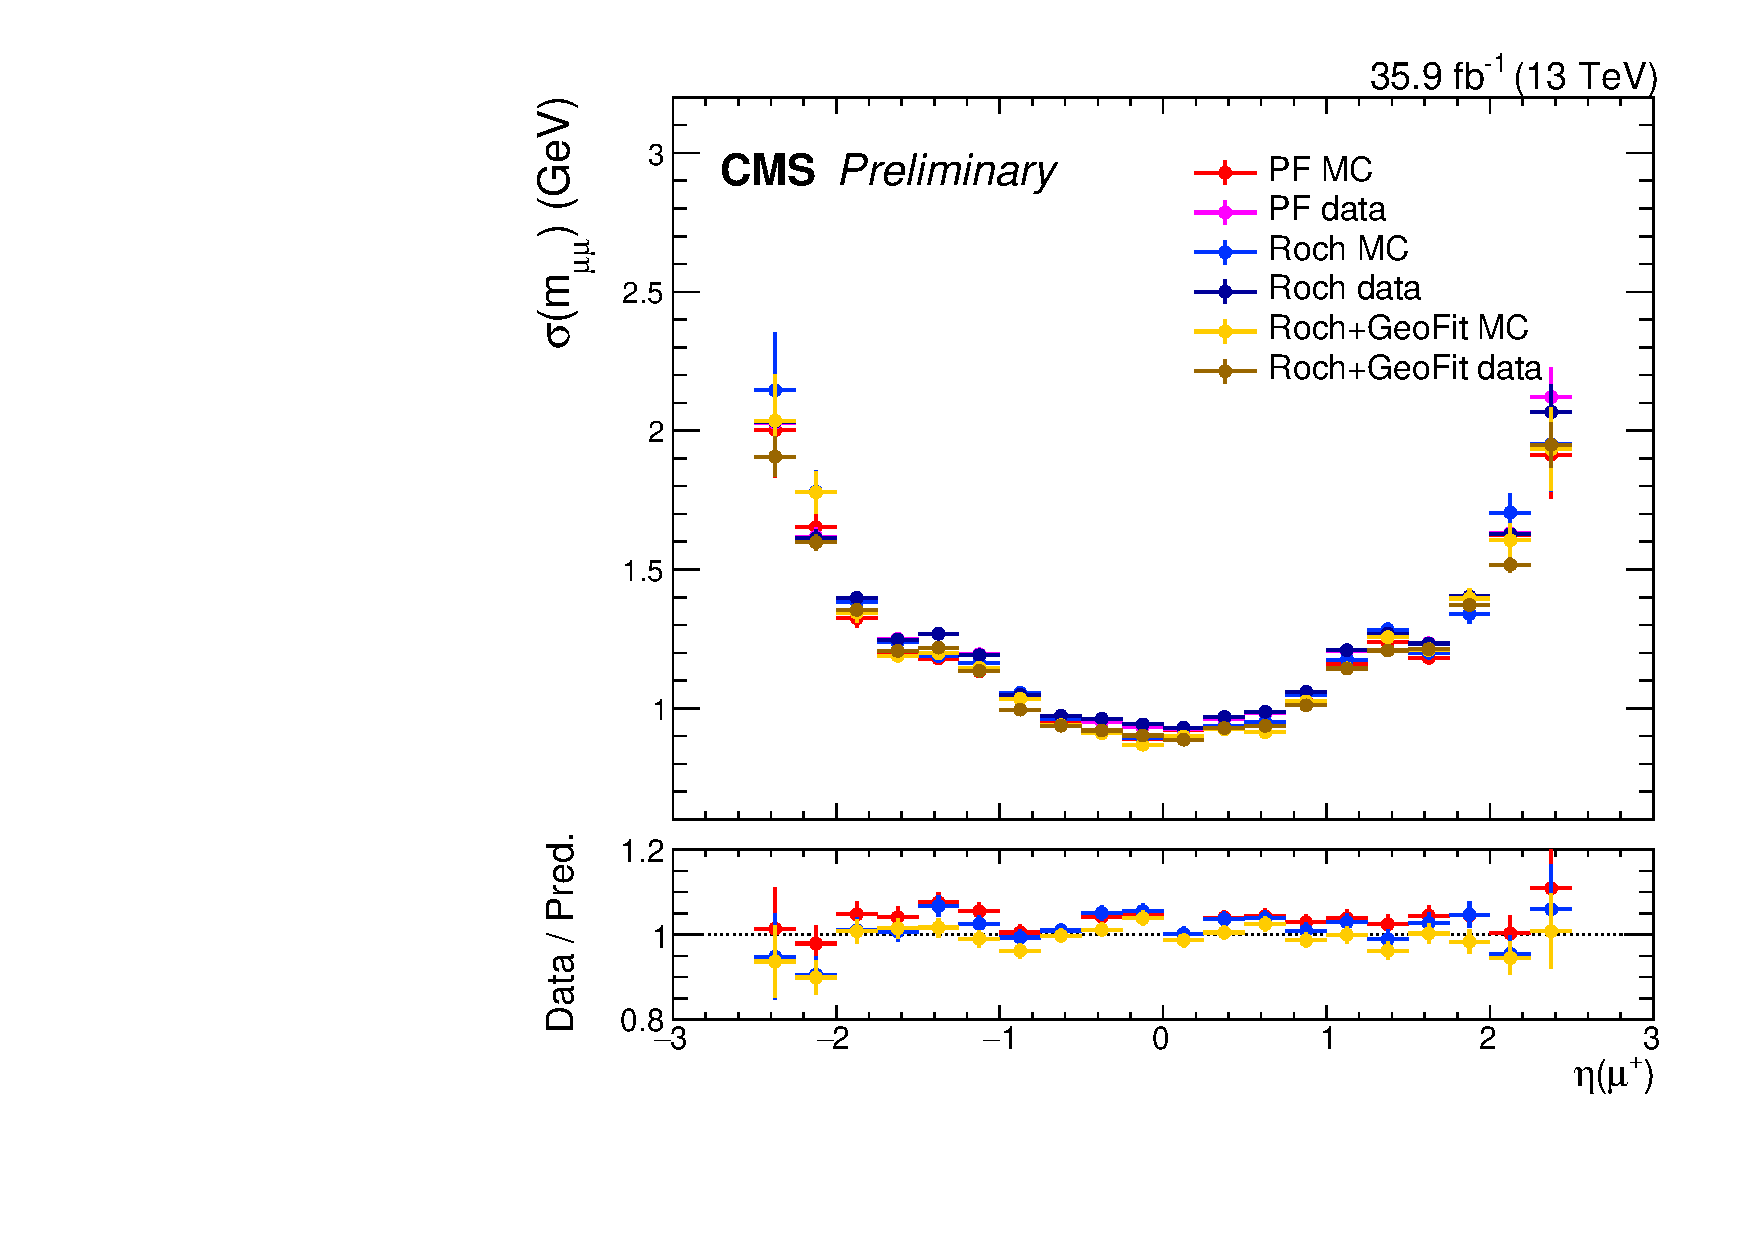
\includegraphics[width=0.32\textwidth]{pics/muon_corr/muon_cal/2016/muP_eta_summary_reso.pdf}
      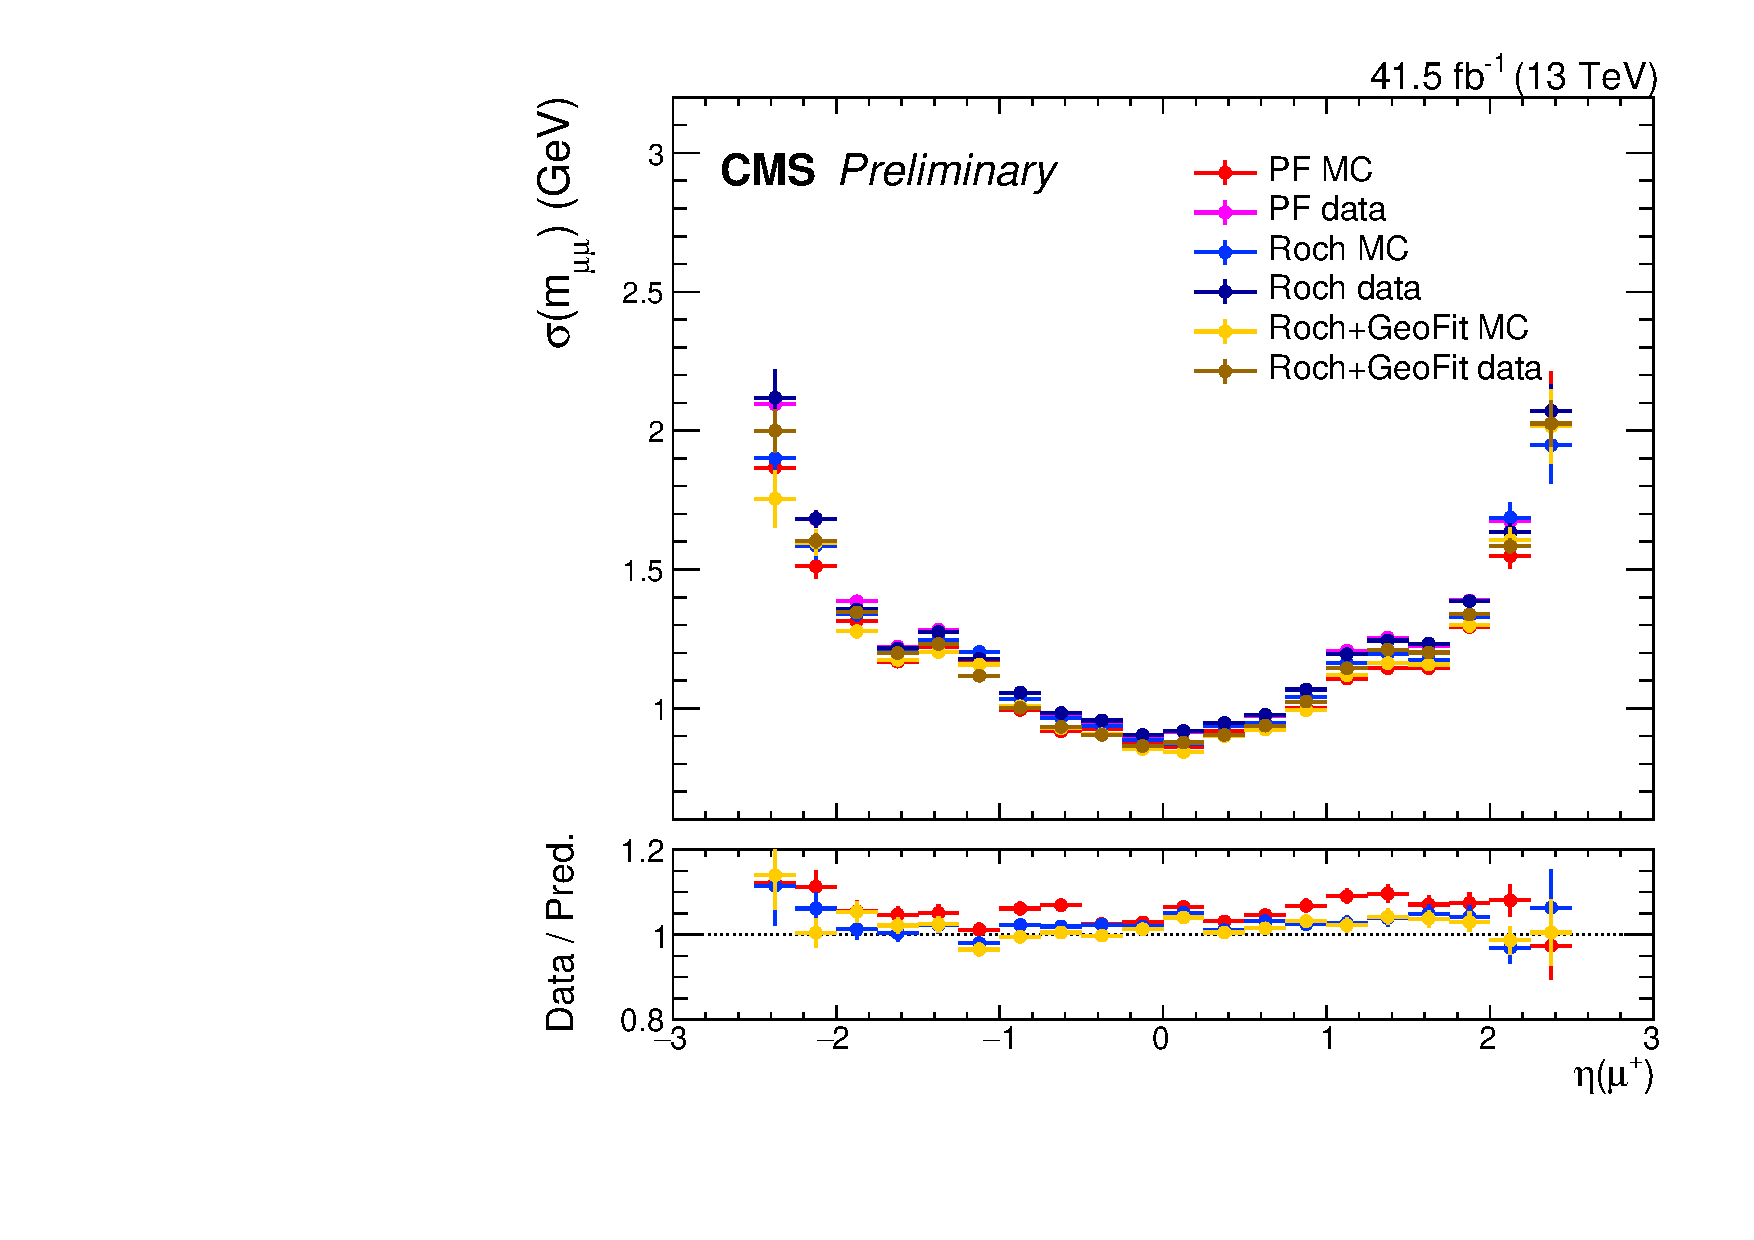
\includegraphics[width=0.32\textwidth]{pics/muon_corr/muon_cal/2017/muP_eta_summary_reso.pdf}
      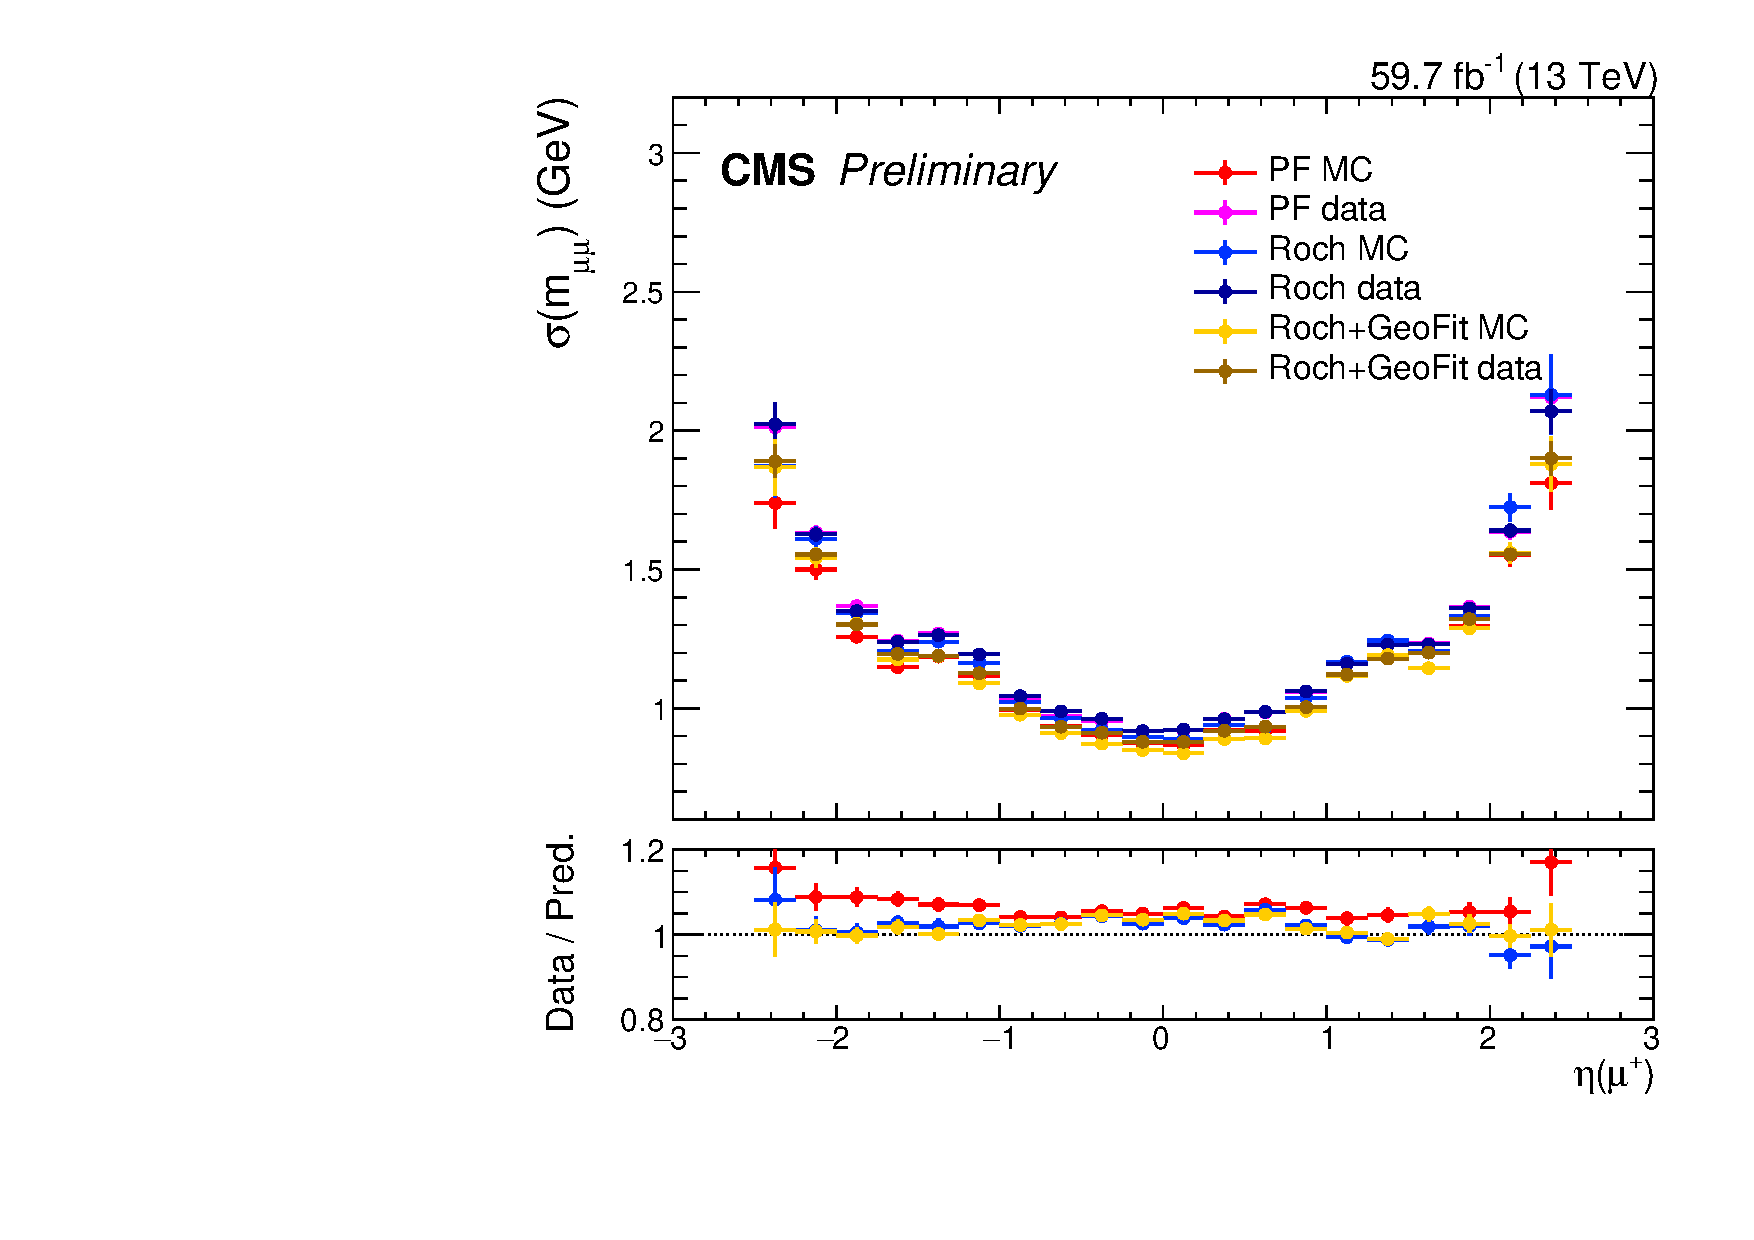
\includegraphics[width=0.32\textwidth]{pics/muon_corr/muon_cal/2018/muP_eta_summary_reso.pdf}
      \caption{Muon calibration plots vs $\eta(\mu^{+})$, for 2016 (left column), 2017 (middle column) and 2018 (right column).
               The top row shows the mean value of the Voigtian fit to the \mmm distribution, 
               while the bottom row shows its experimental resolution.}
      \label{fig:mucal_muP_eta}
\end{figure*}


\begin{figure*}[!htb]
      \centering
%      \captionsetup{justification=justified}
      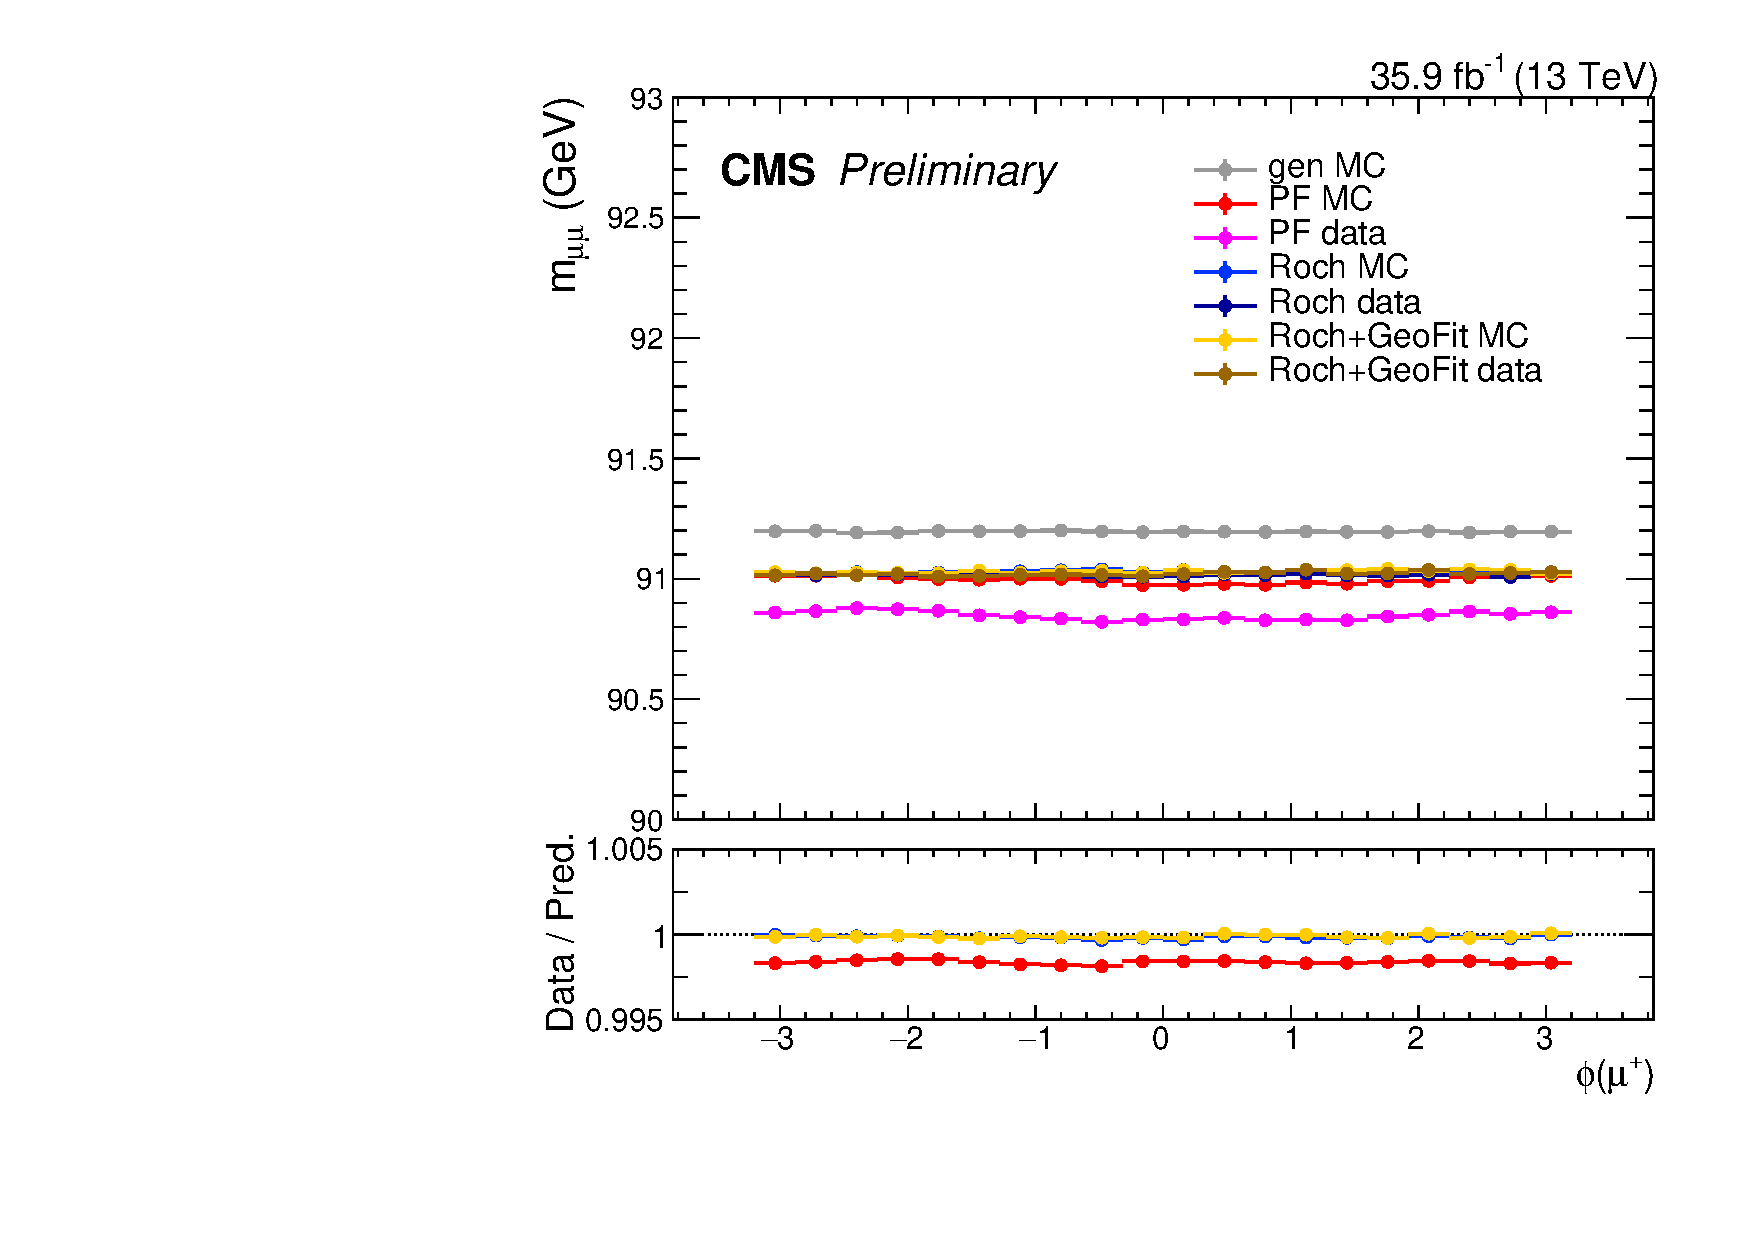
\includegraphics[width=0.32\textwidth]{pics/muon_corr/muon_cal/2016/muP_phi_summary_mean.pdf}
      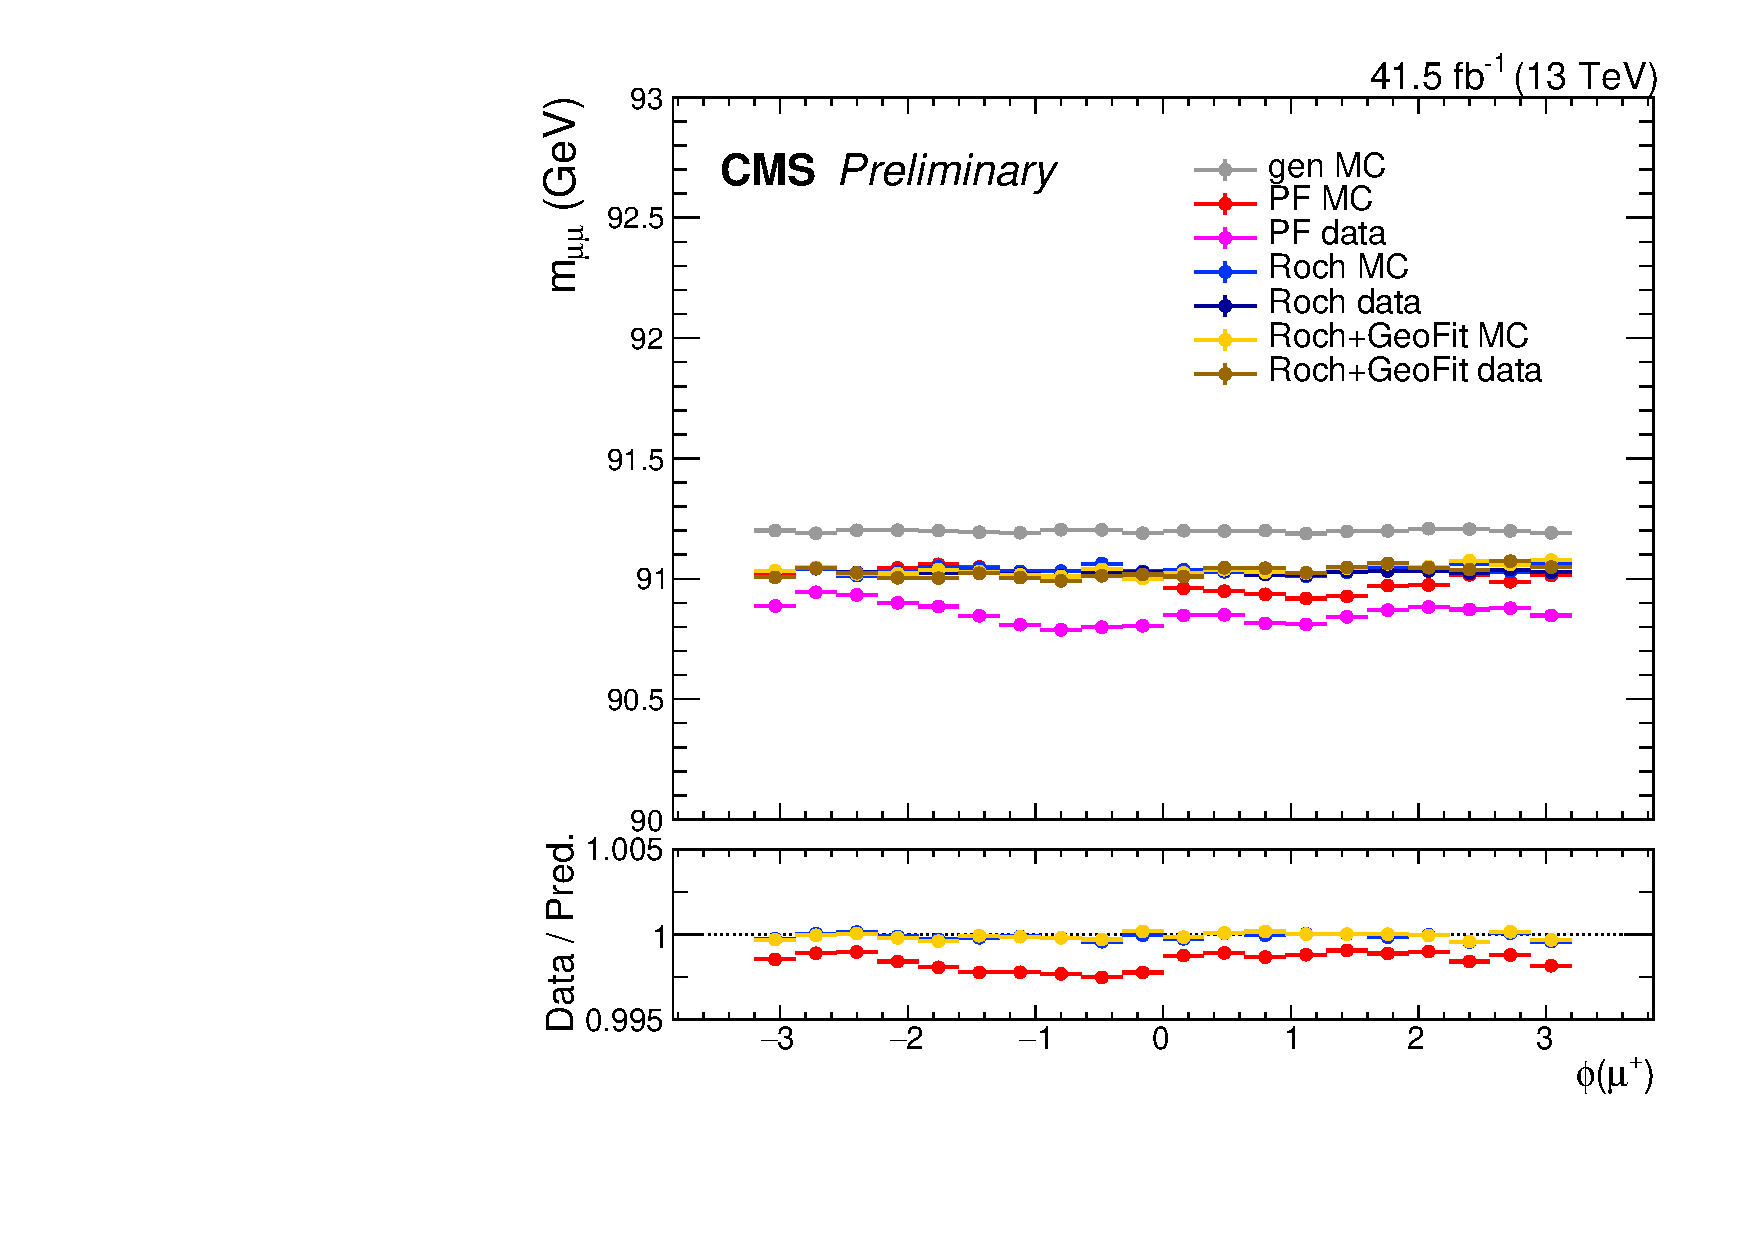
\includegraphics[width=0.32\textwidth]{pics/muon_corr/muon_cal/2017/muP_phi_summary_mean.pdf}
      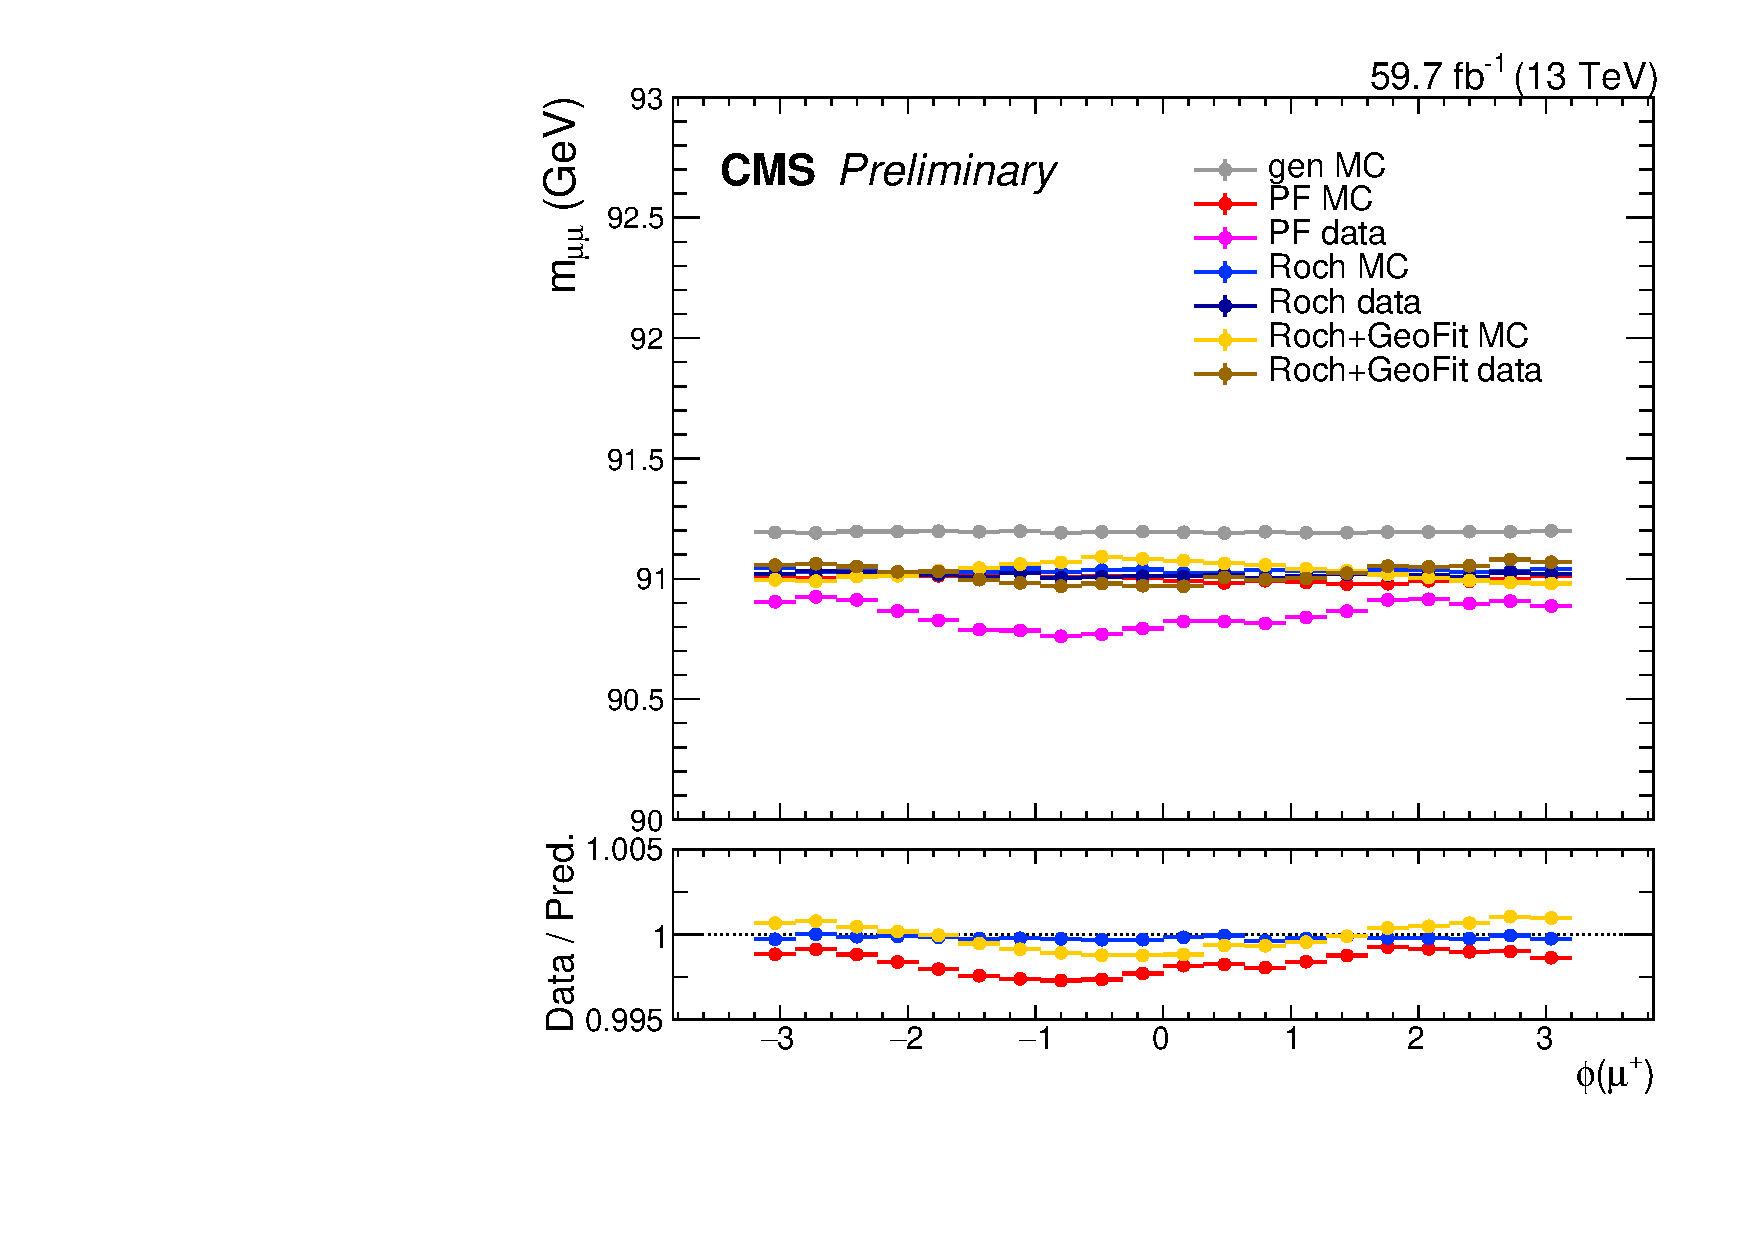
\includegraphics[width=0.32\textwidth]{pics/muon_corr/muon_cal/2018/muP_phi_summary_mean.pdf}
      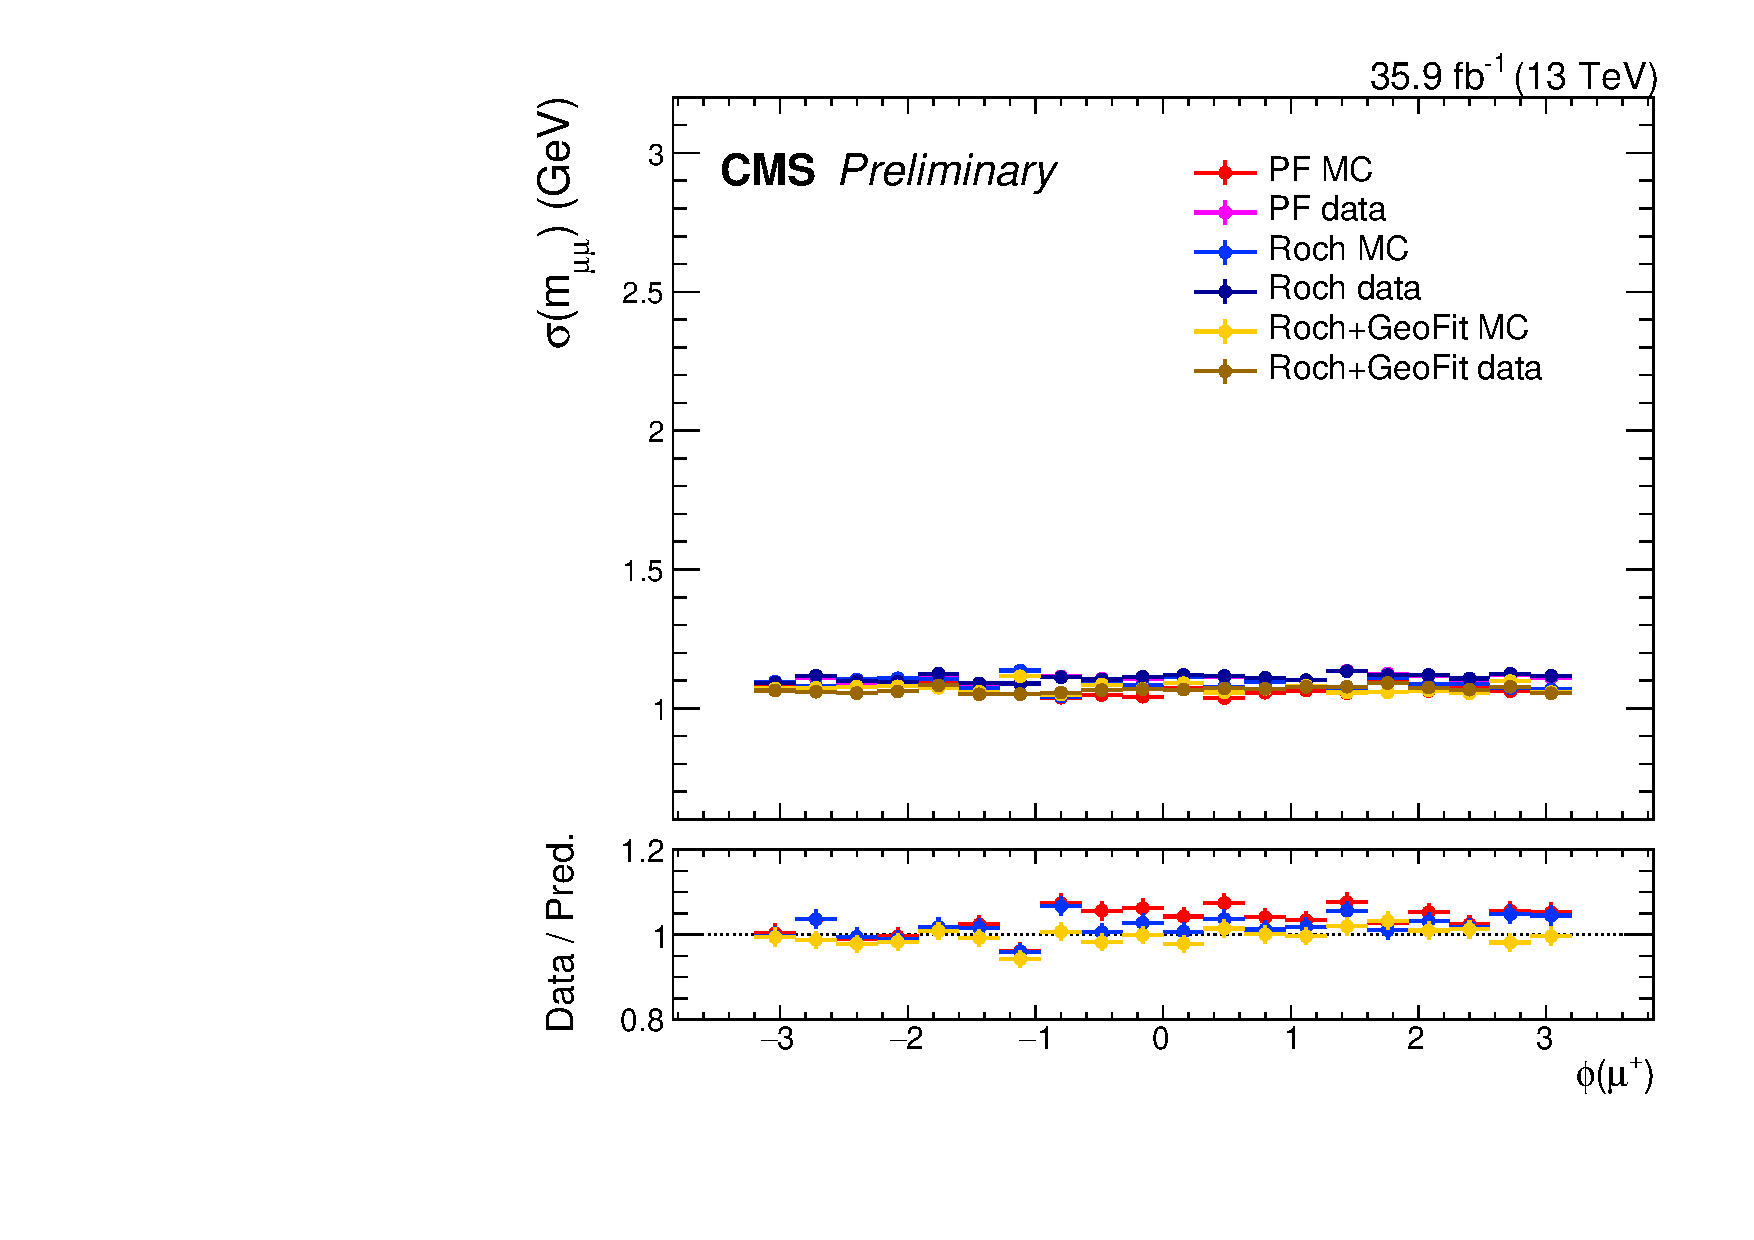
\includegraphics[width=0.32\textwidth]{pics/muon_corr/muon_cal/2016/muP_phi_summary_reso.pdf}
      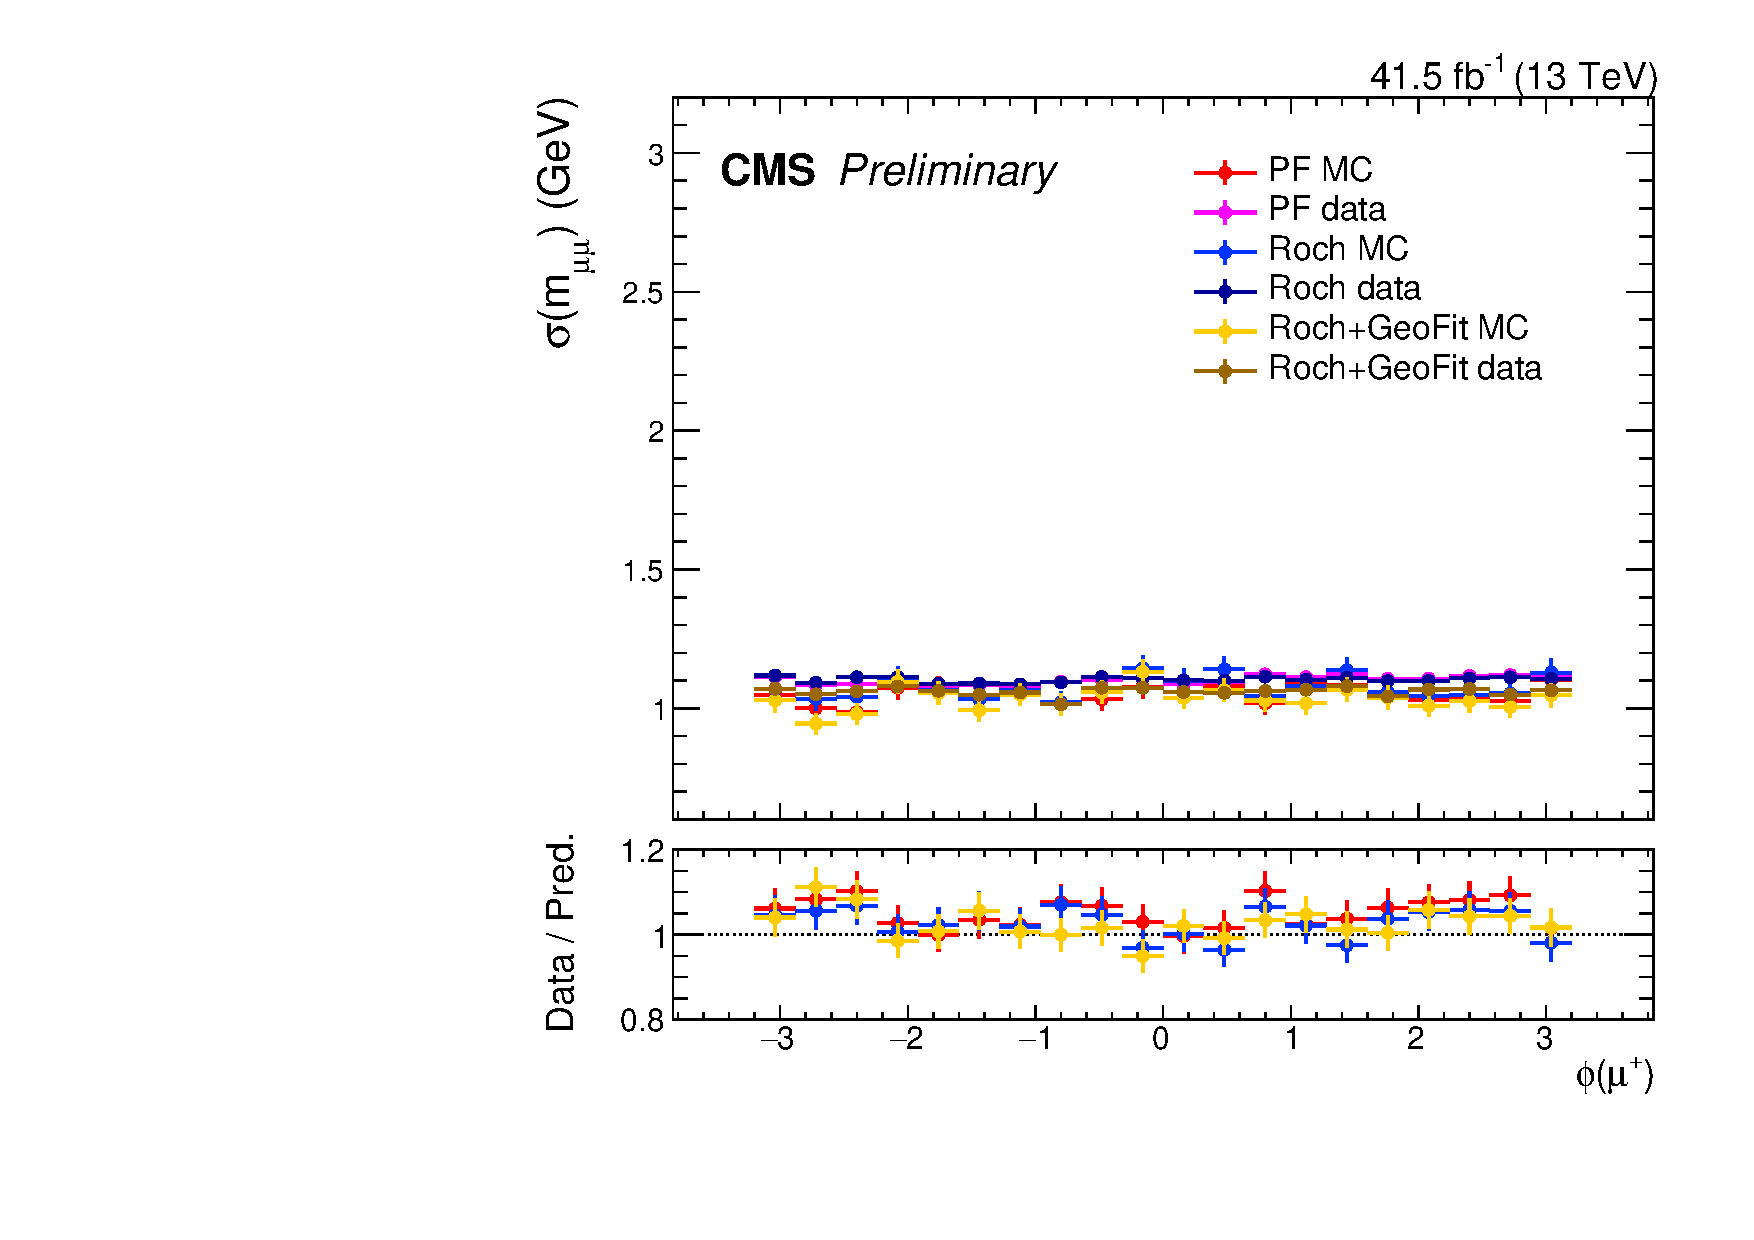
\includegraphics[width=0.32\textwidth]{pics/muon_corr/muon_cal/2017/muP_phi_summary_reso.pdf}
      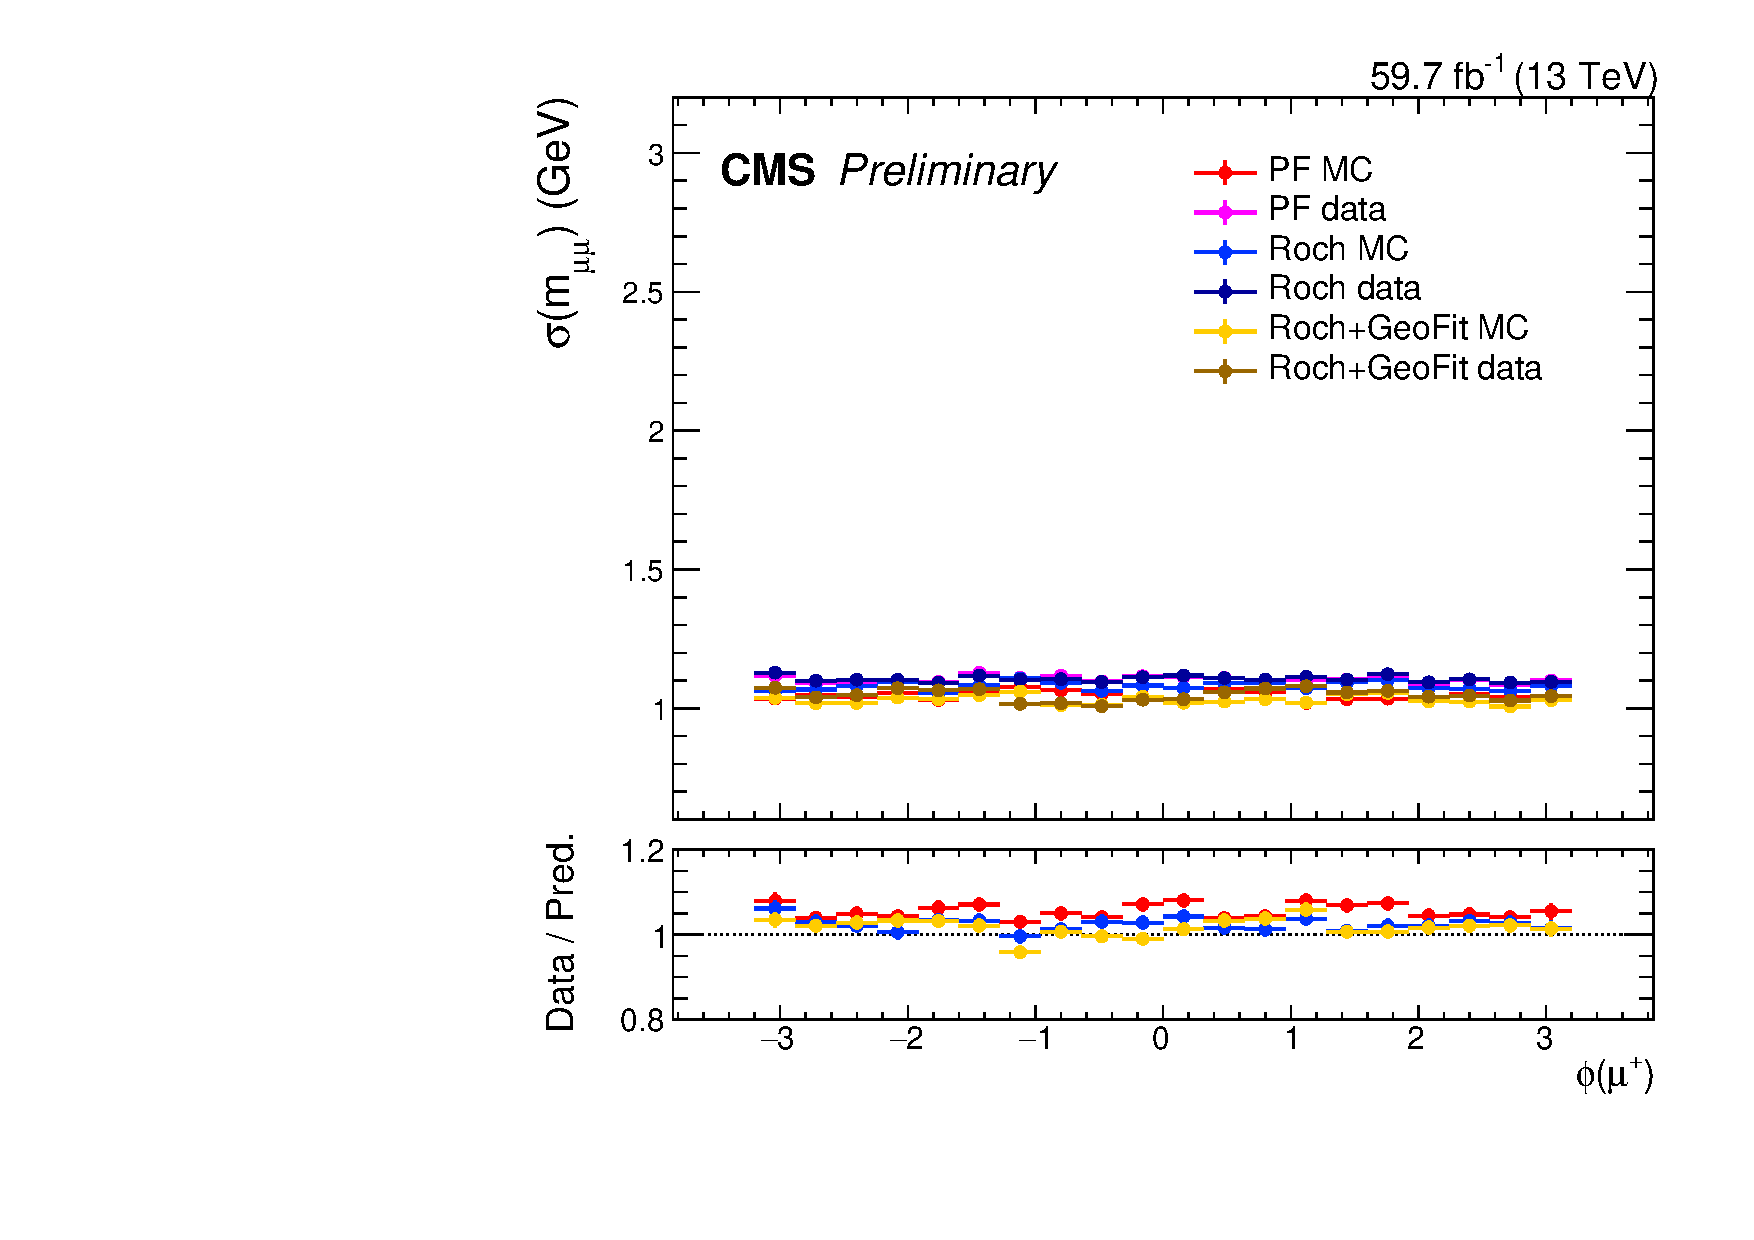
\includegraphics[width=0.32\textwidth]{pics/muon_corr/muon_cal/2018/muP_phi_summary_reso.pdf}
      \caption{Muon calibration plots vs $\phi(\mu^{+})$, for 2016 (left column), 2017 (middle column) and 2018 (right column).
              The top row shows the mean value of the Voigtian fit to the \mmm distribution, 
              while the bottom row shows its experimental resolution.}
      \label{fig:mucal_muP_phi}
\end{figure*}


\begin{figure*}[!htb]
      \centering
%      \captionsetup{justification=justified}
      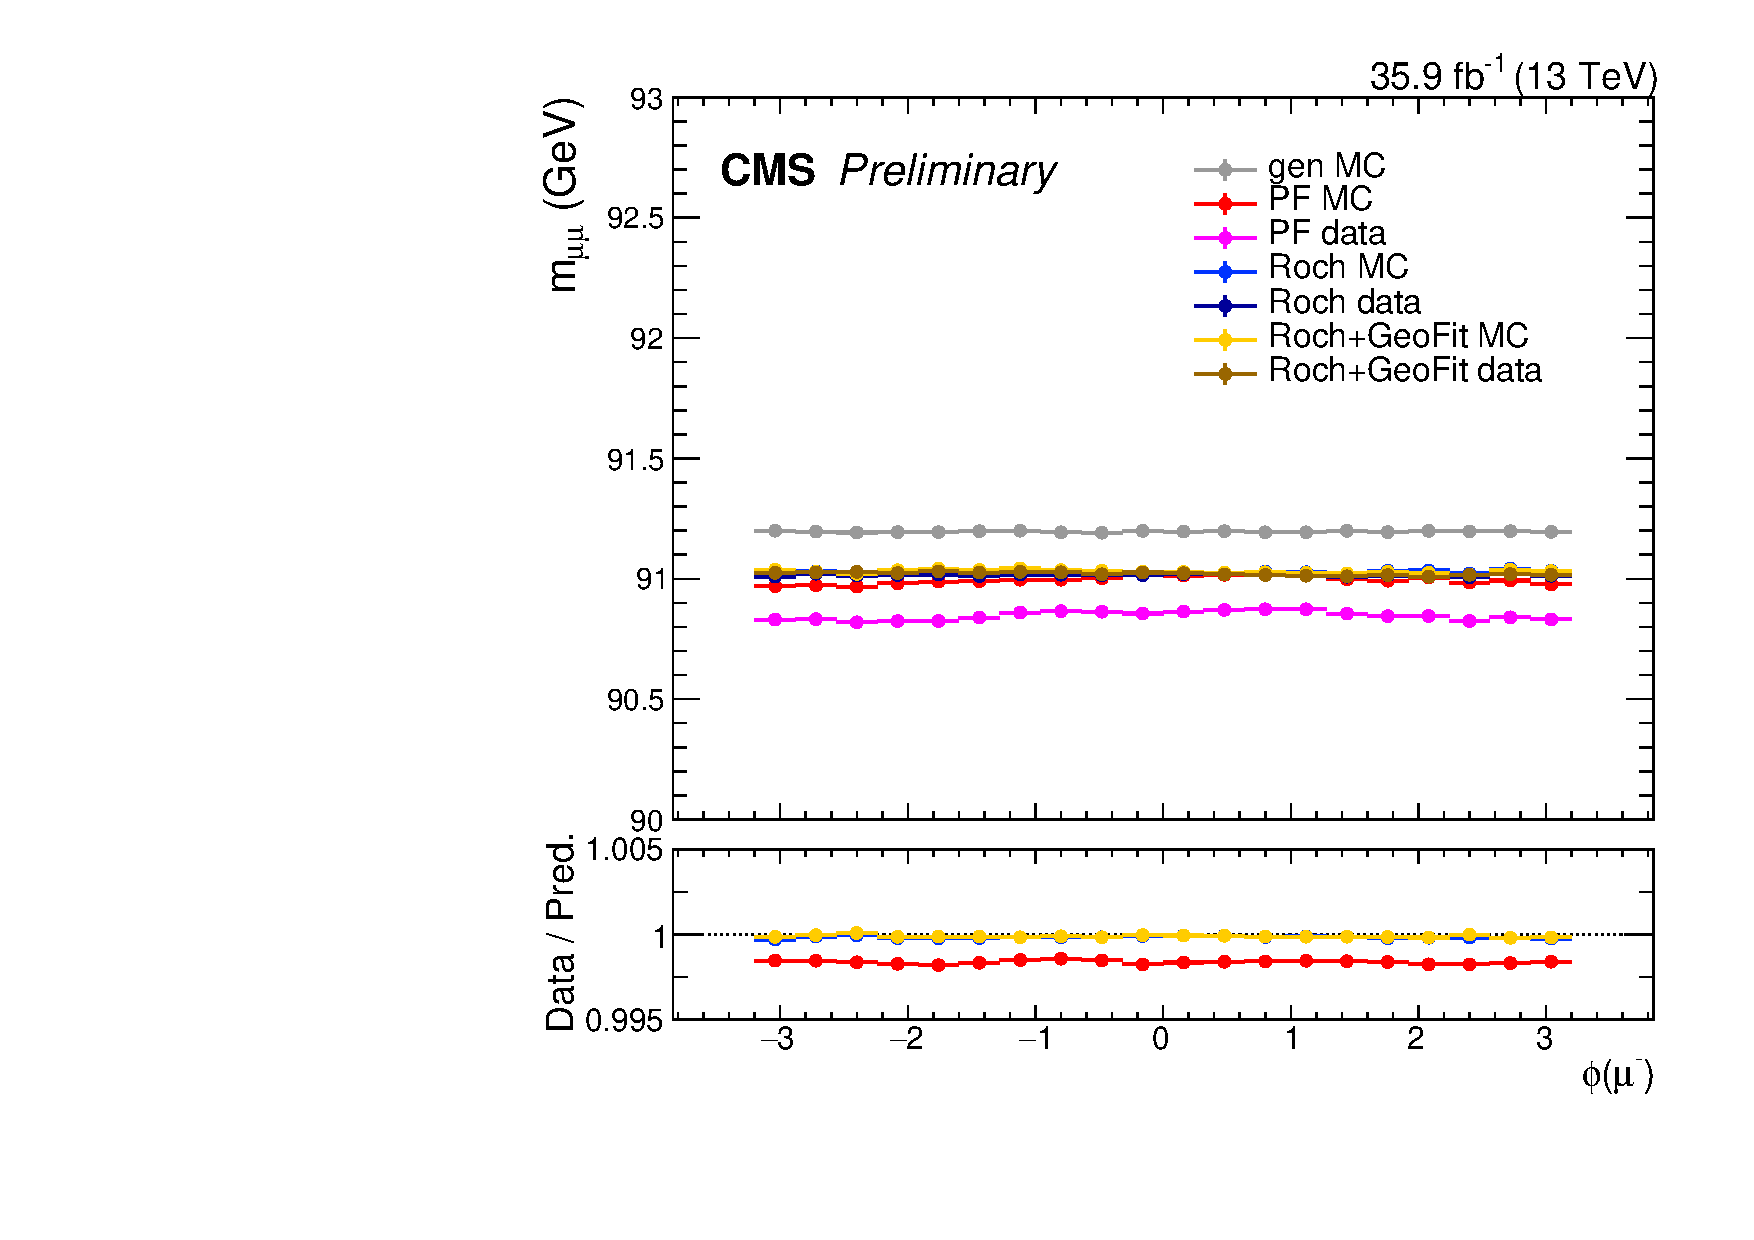
\includegraphics[width=0.32\textwidth]{pics/muon_corr/muon_cal/2016/muN_phi_summary_mean.pdf}
      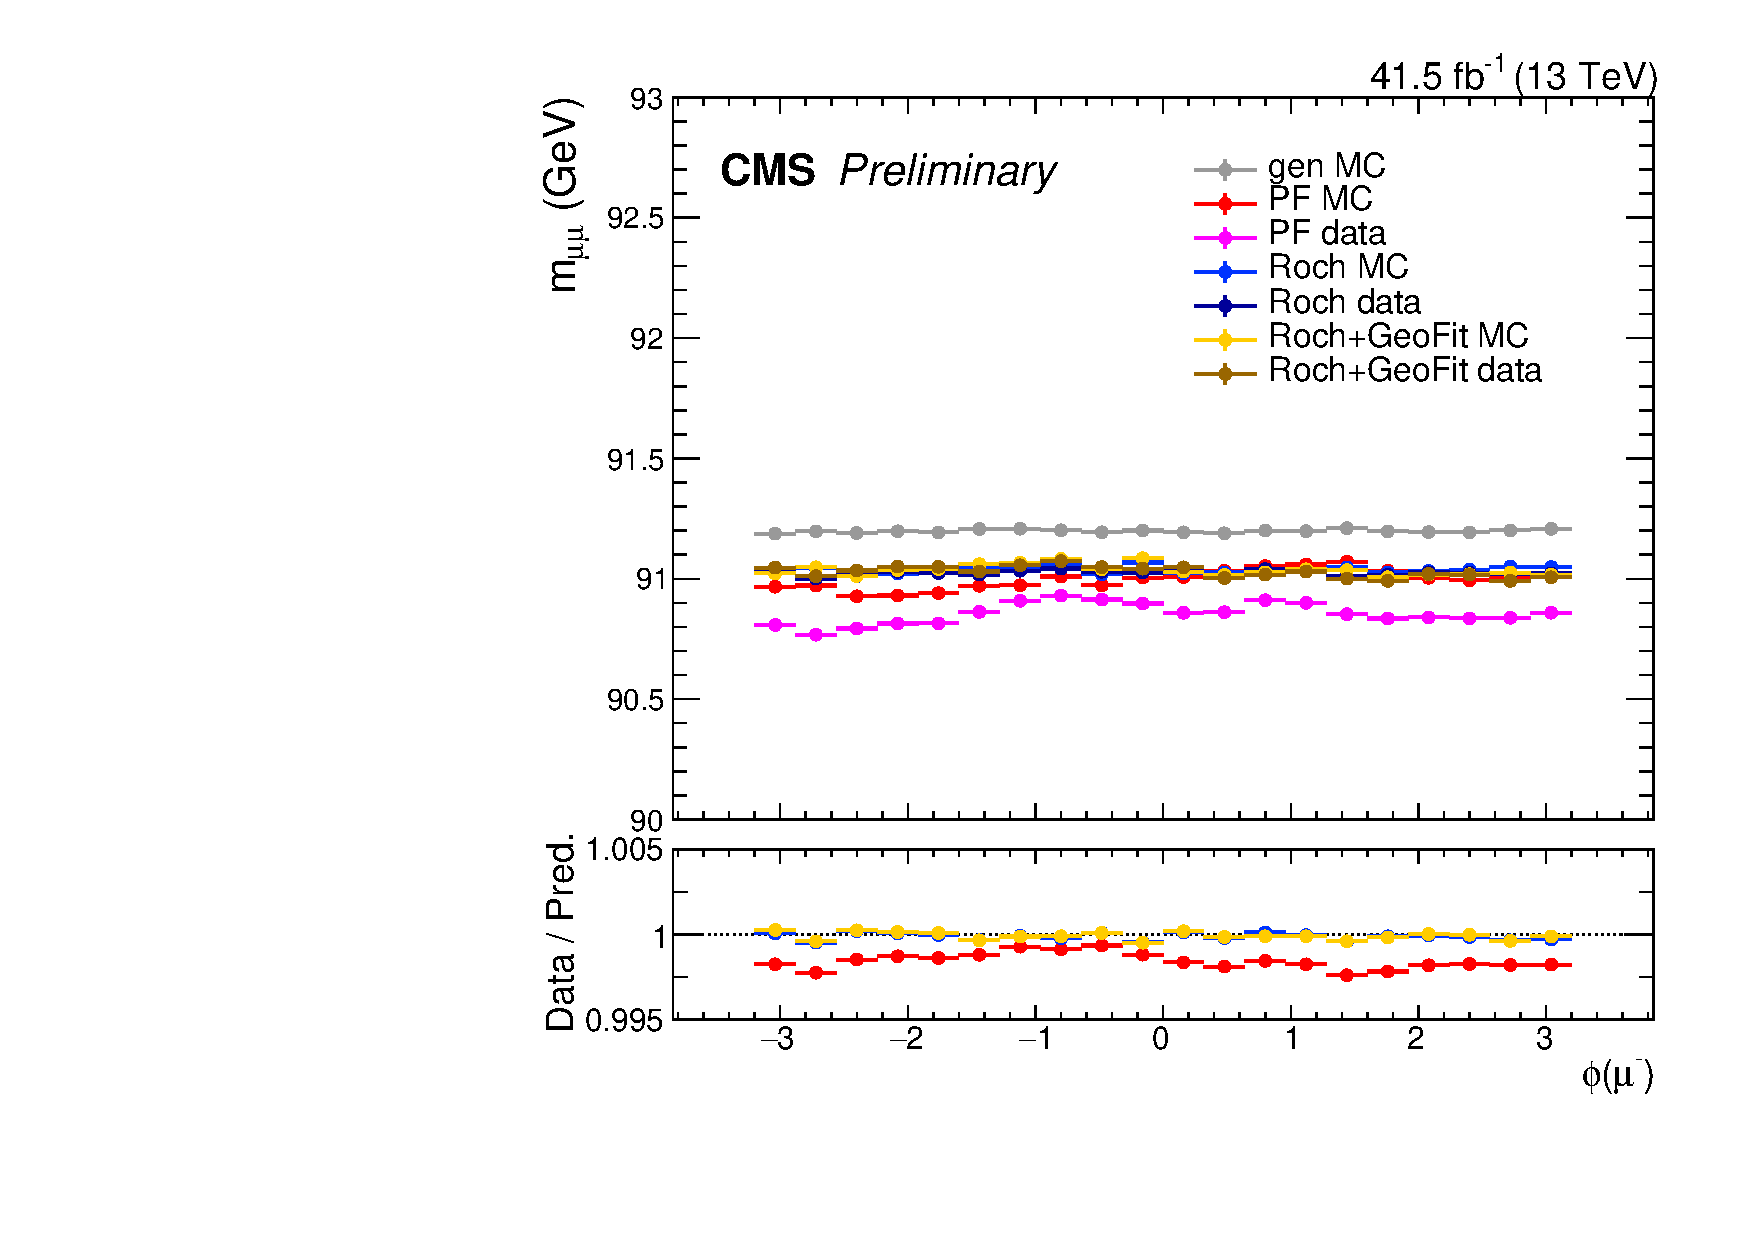
\includegraphics[width=0.32\textwidth]{pics/muon_corr/muon_cal/2017/muN_phi_summary_mean.pdf}
      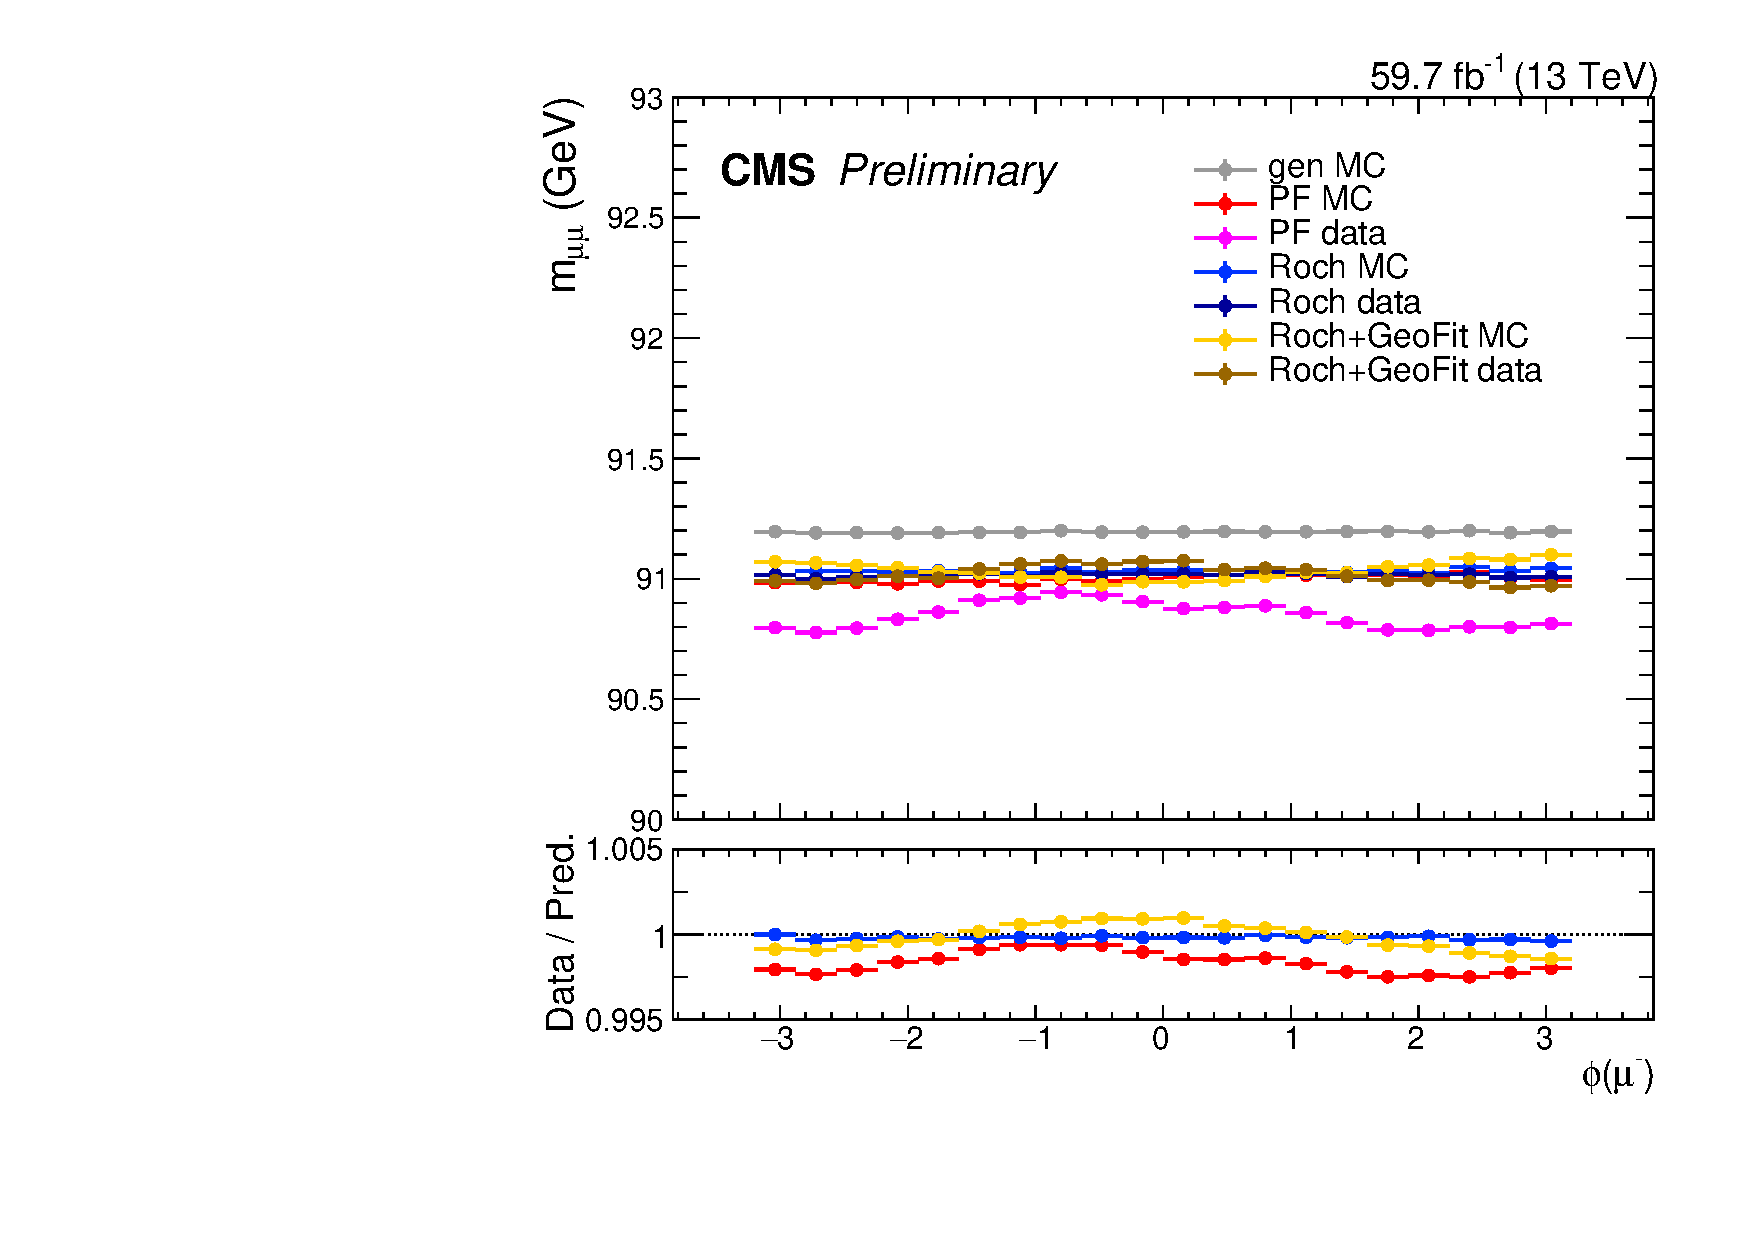
\includegraphics[width=0.32\textwidth]{pics/muon_corr/muon_cal/2018/muN_phi_summary_mean.pdf}
      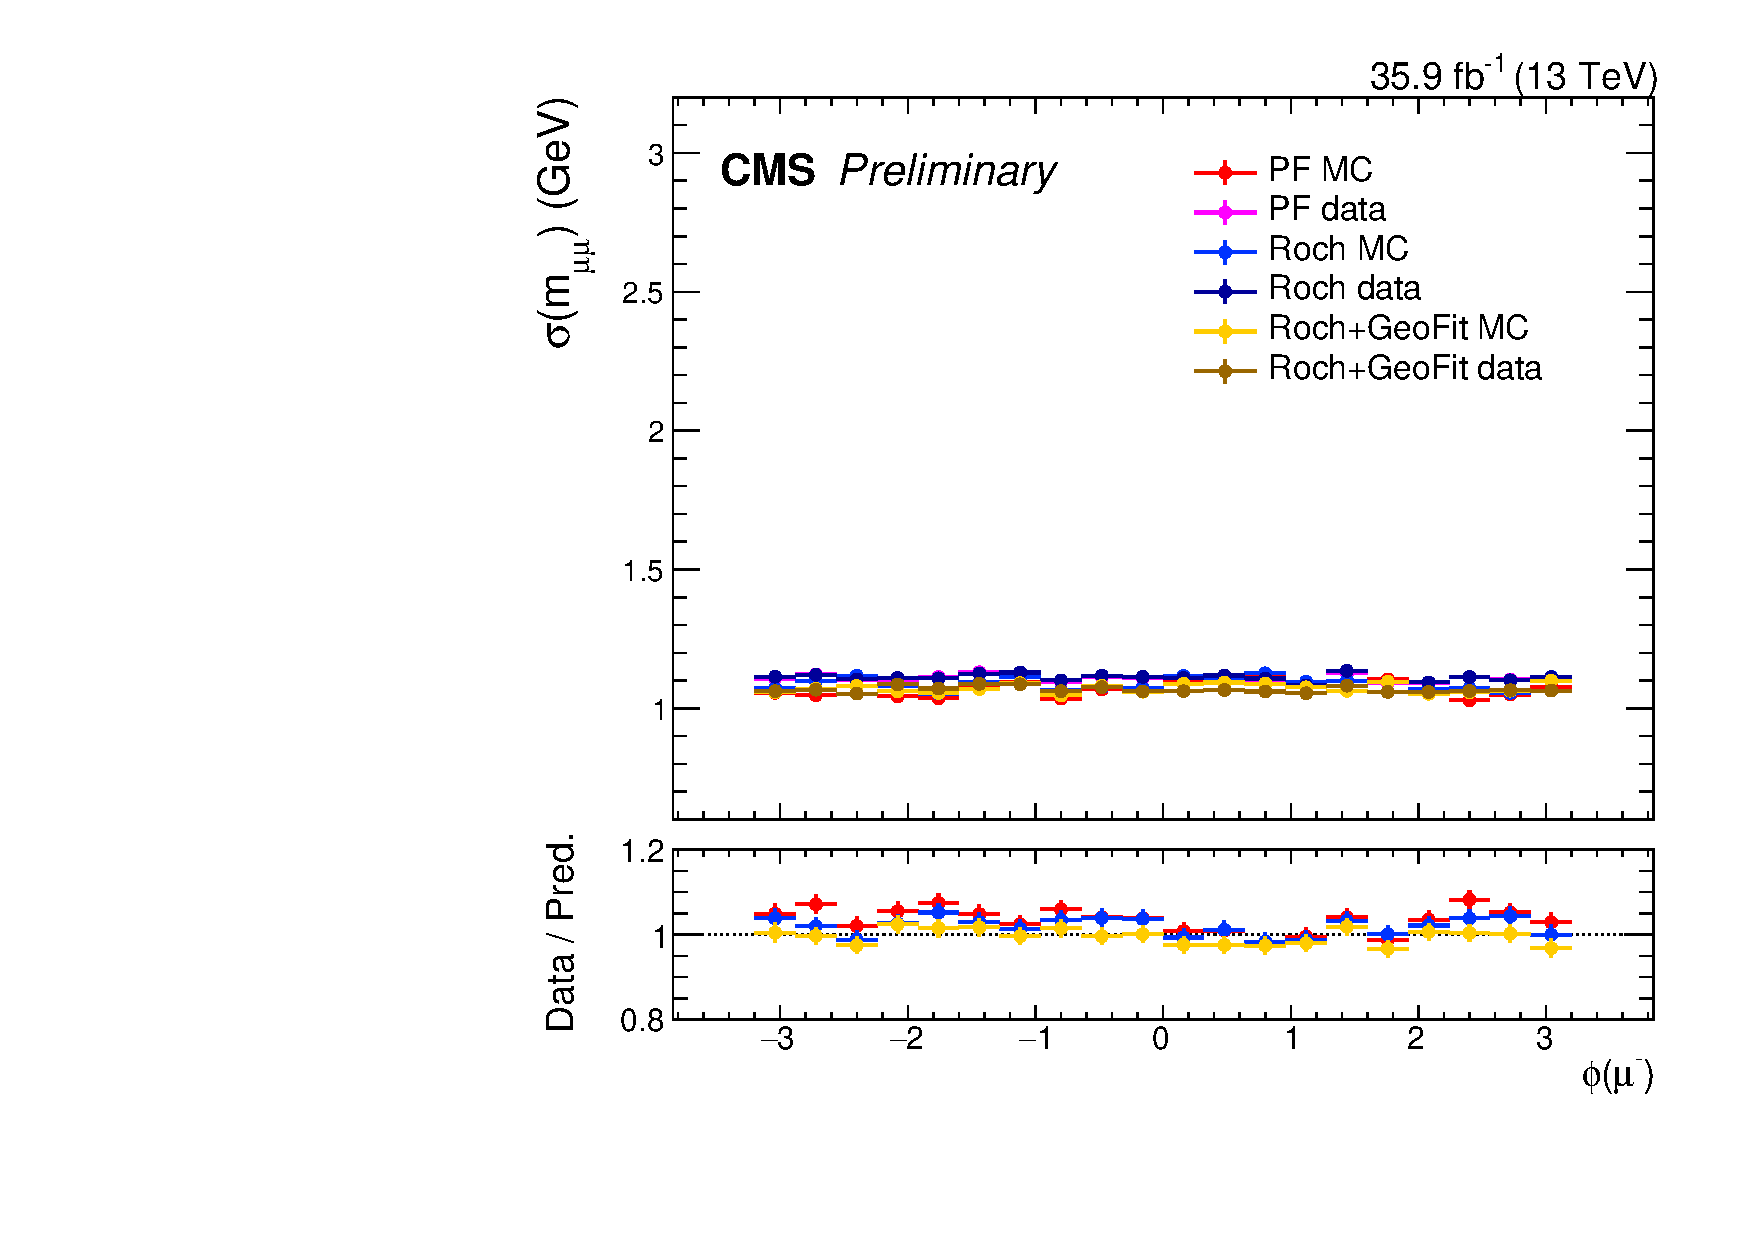
\includegraphics[width=0.32\textwidth]{pics/muon_corr/muon_cal/2016/muN_phi_summary_reso.pdf}
      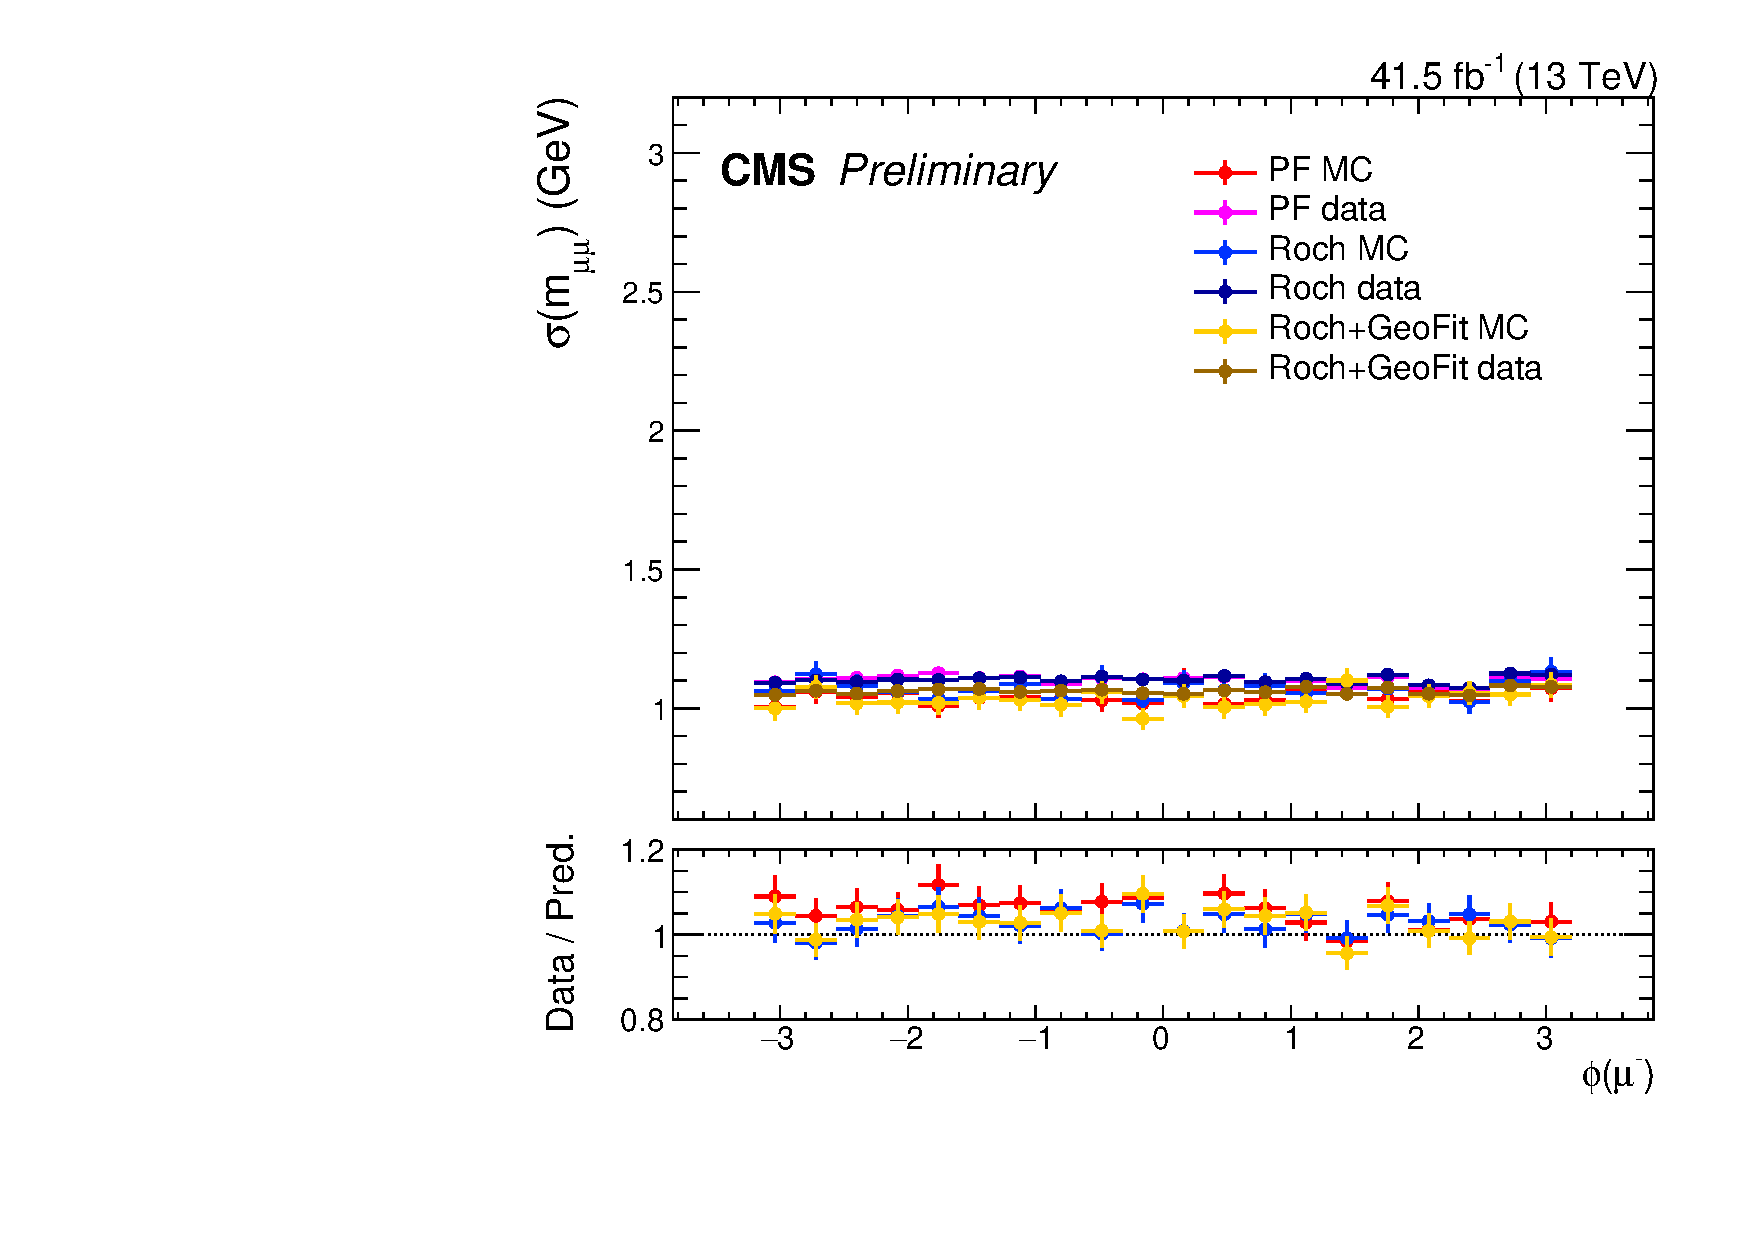
\includegraphics[width=0.32\textwidth]{pics/muon_corr/muon_cal/2017/muN_phi_summary_reso.pdf}
      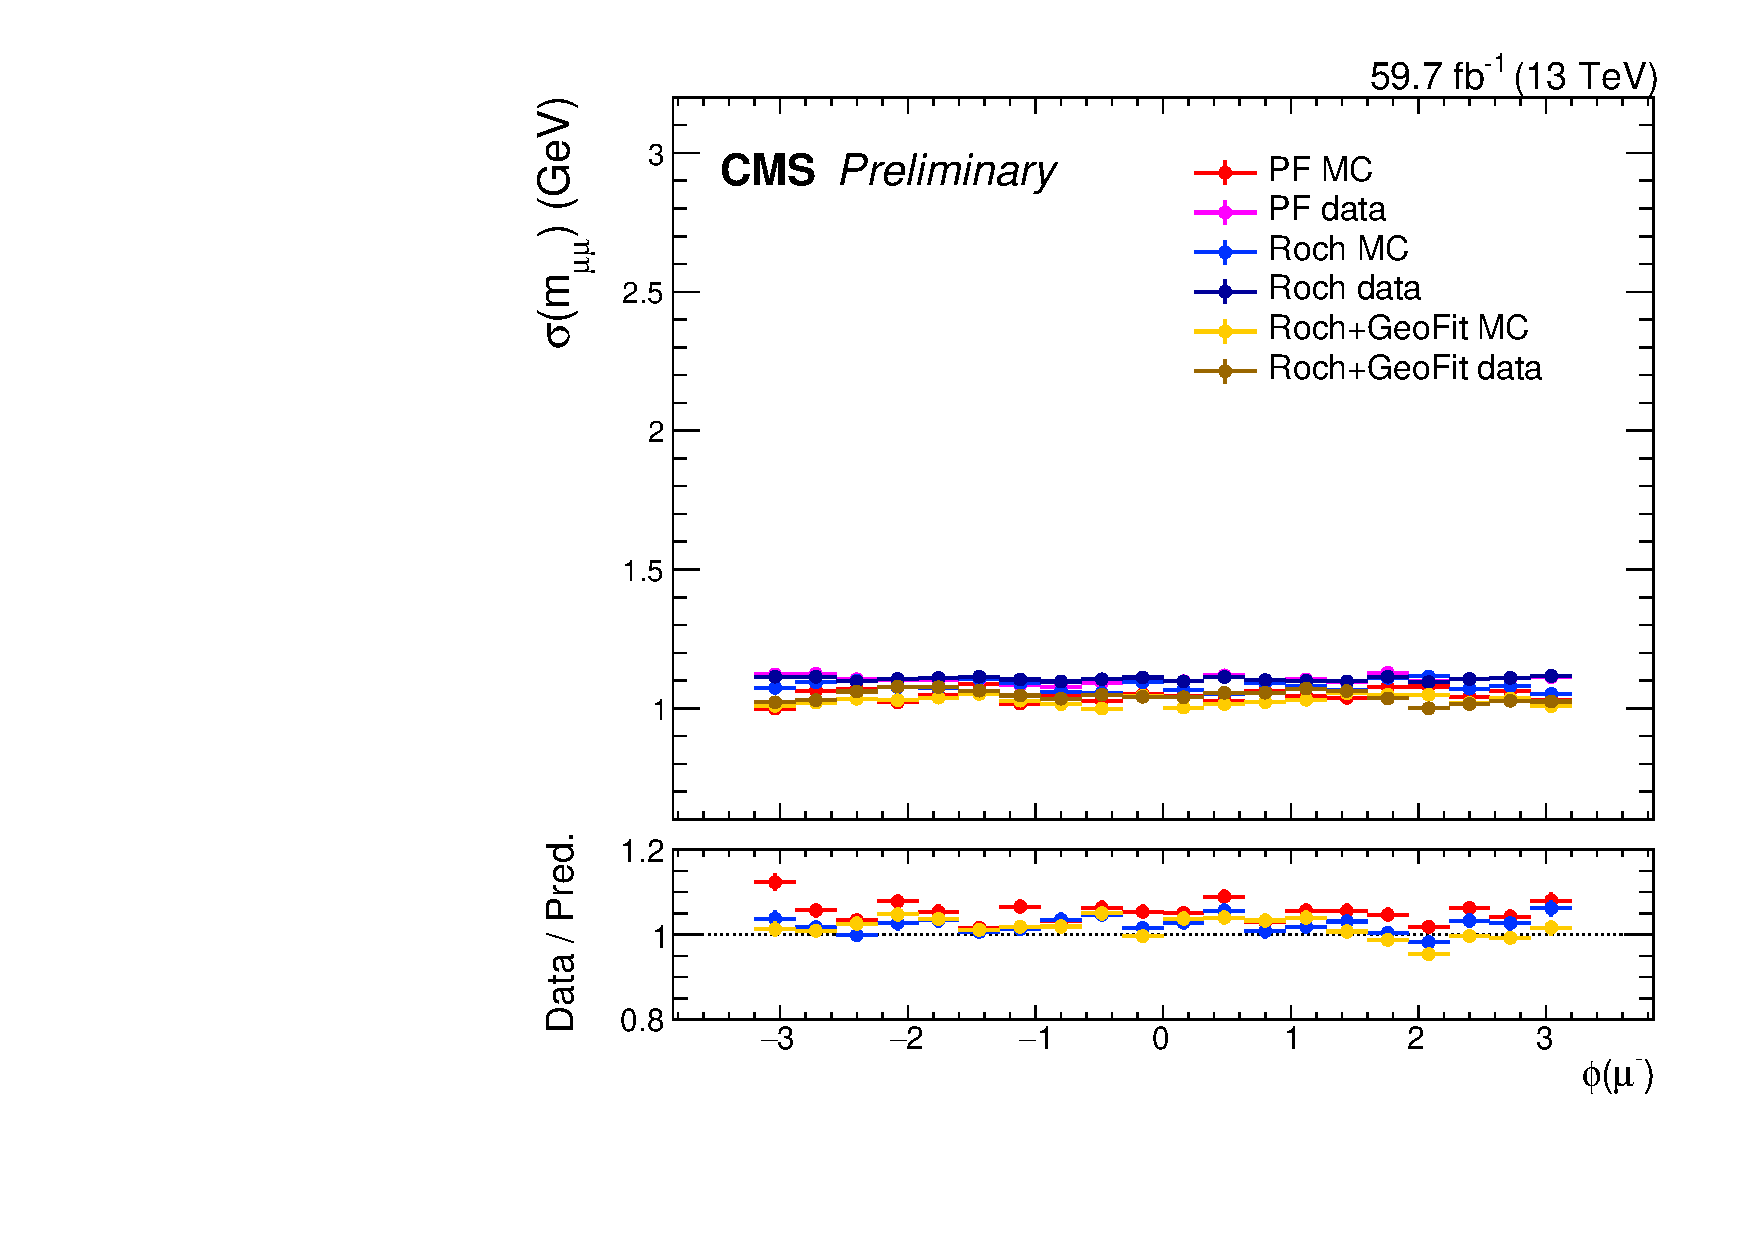
\includegraphics[width=0.32\textwidth]{pics/muon_corr/muon_cal/2018/muN_phi_summary_reso.pdf}
      \caption{Muon calibration plots vs $\phi(\mu^{-})$, for 2016 (left column), 2017 (middle column) and 2018 (right column).
               The top row shows the mean value of the Voigtian fit to the \mmm distribution, 
               while the bottom row shows its experimental resolution.}
      \label{fig:mucal_muN_phi}
\end{figure*}


\begin{figure*}[!htb]
      \centering
%      \captionsetup{justification=justified}
      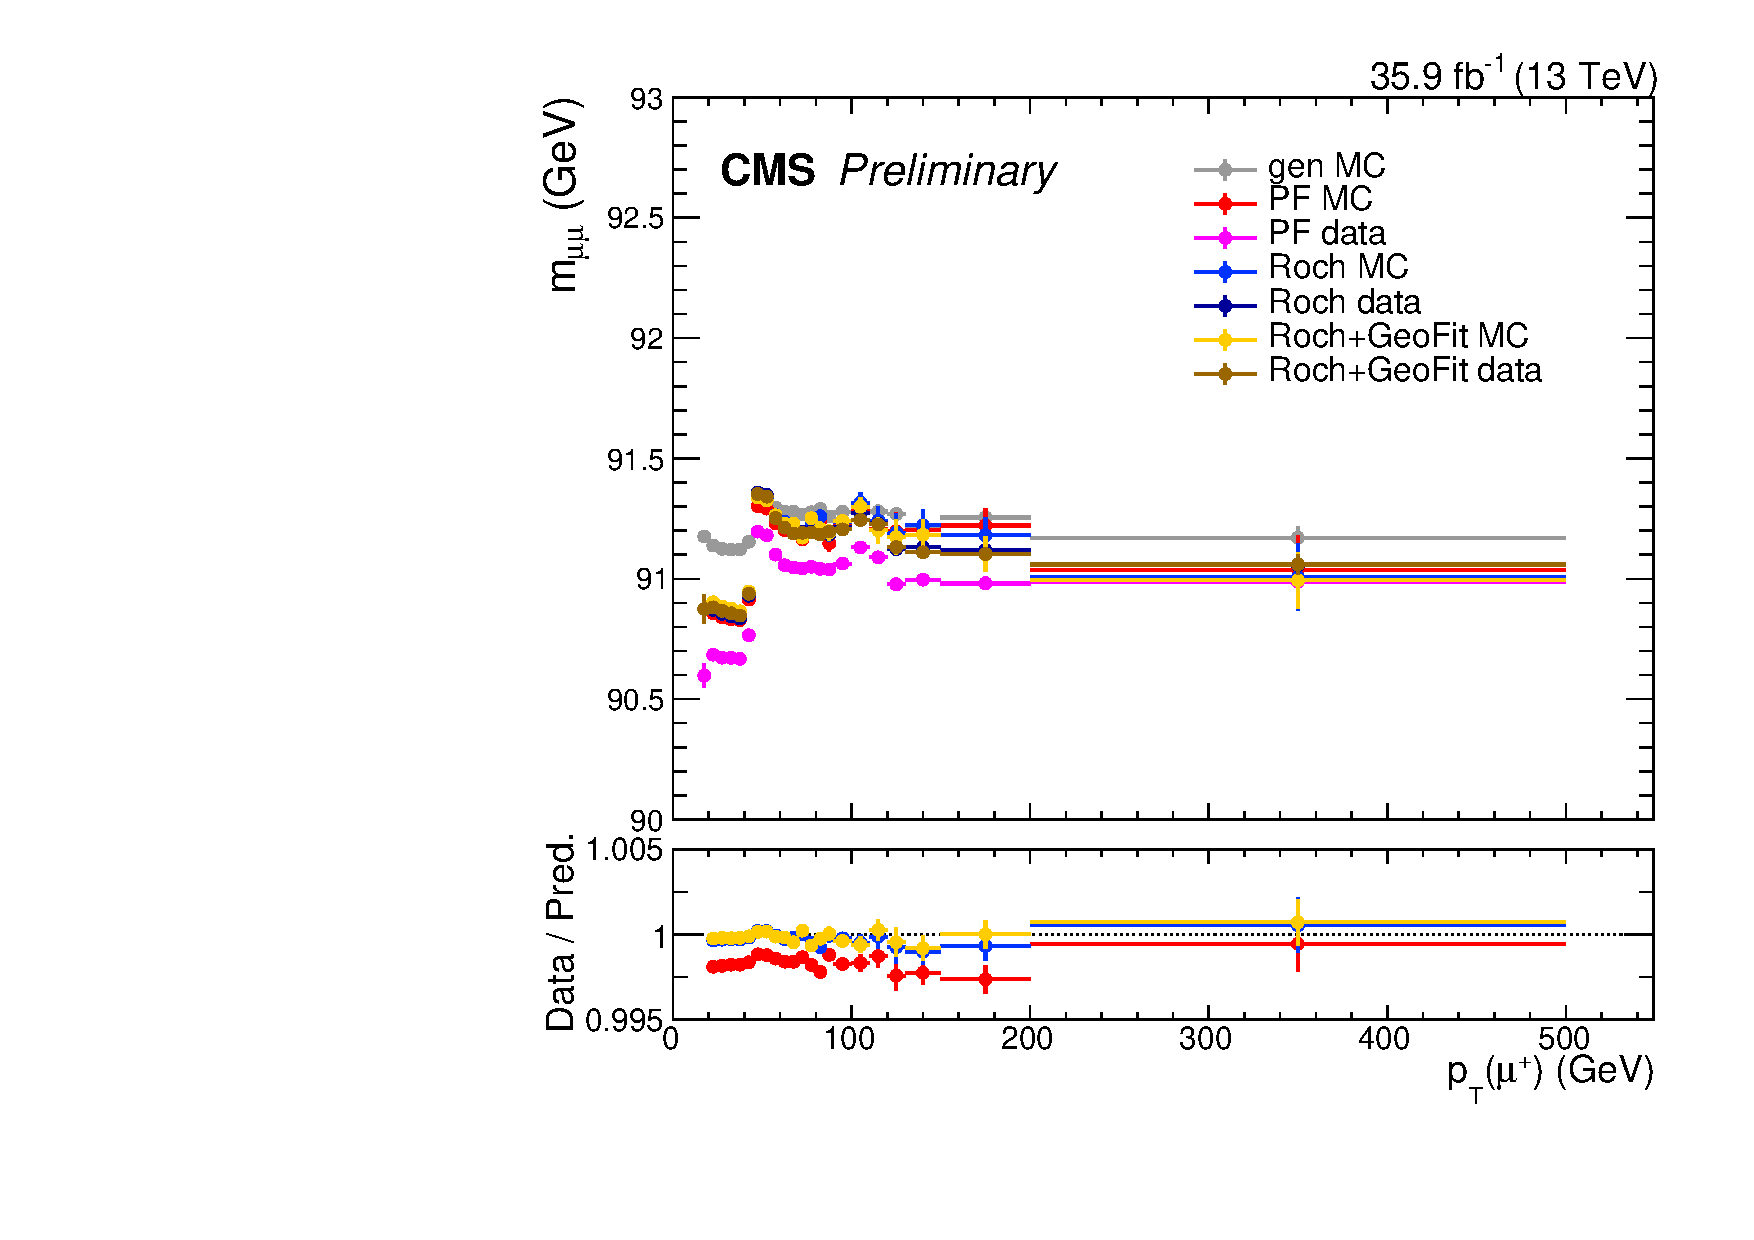
\includegraphics[width=0.32\textwidth]{pics/muon_corr/muon_cal/2016/muP_pt_summary_mean.pdf}
      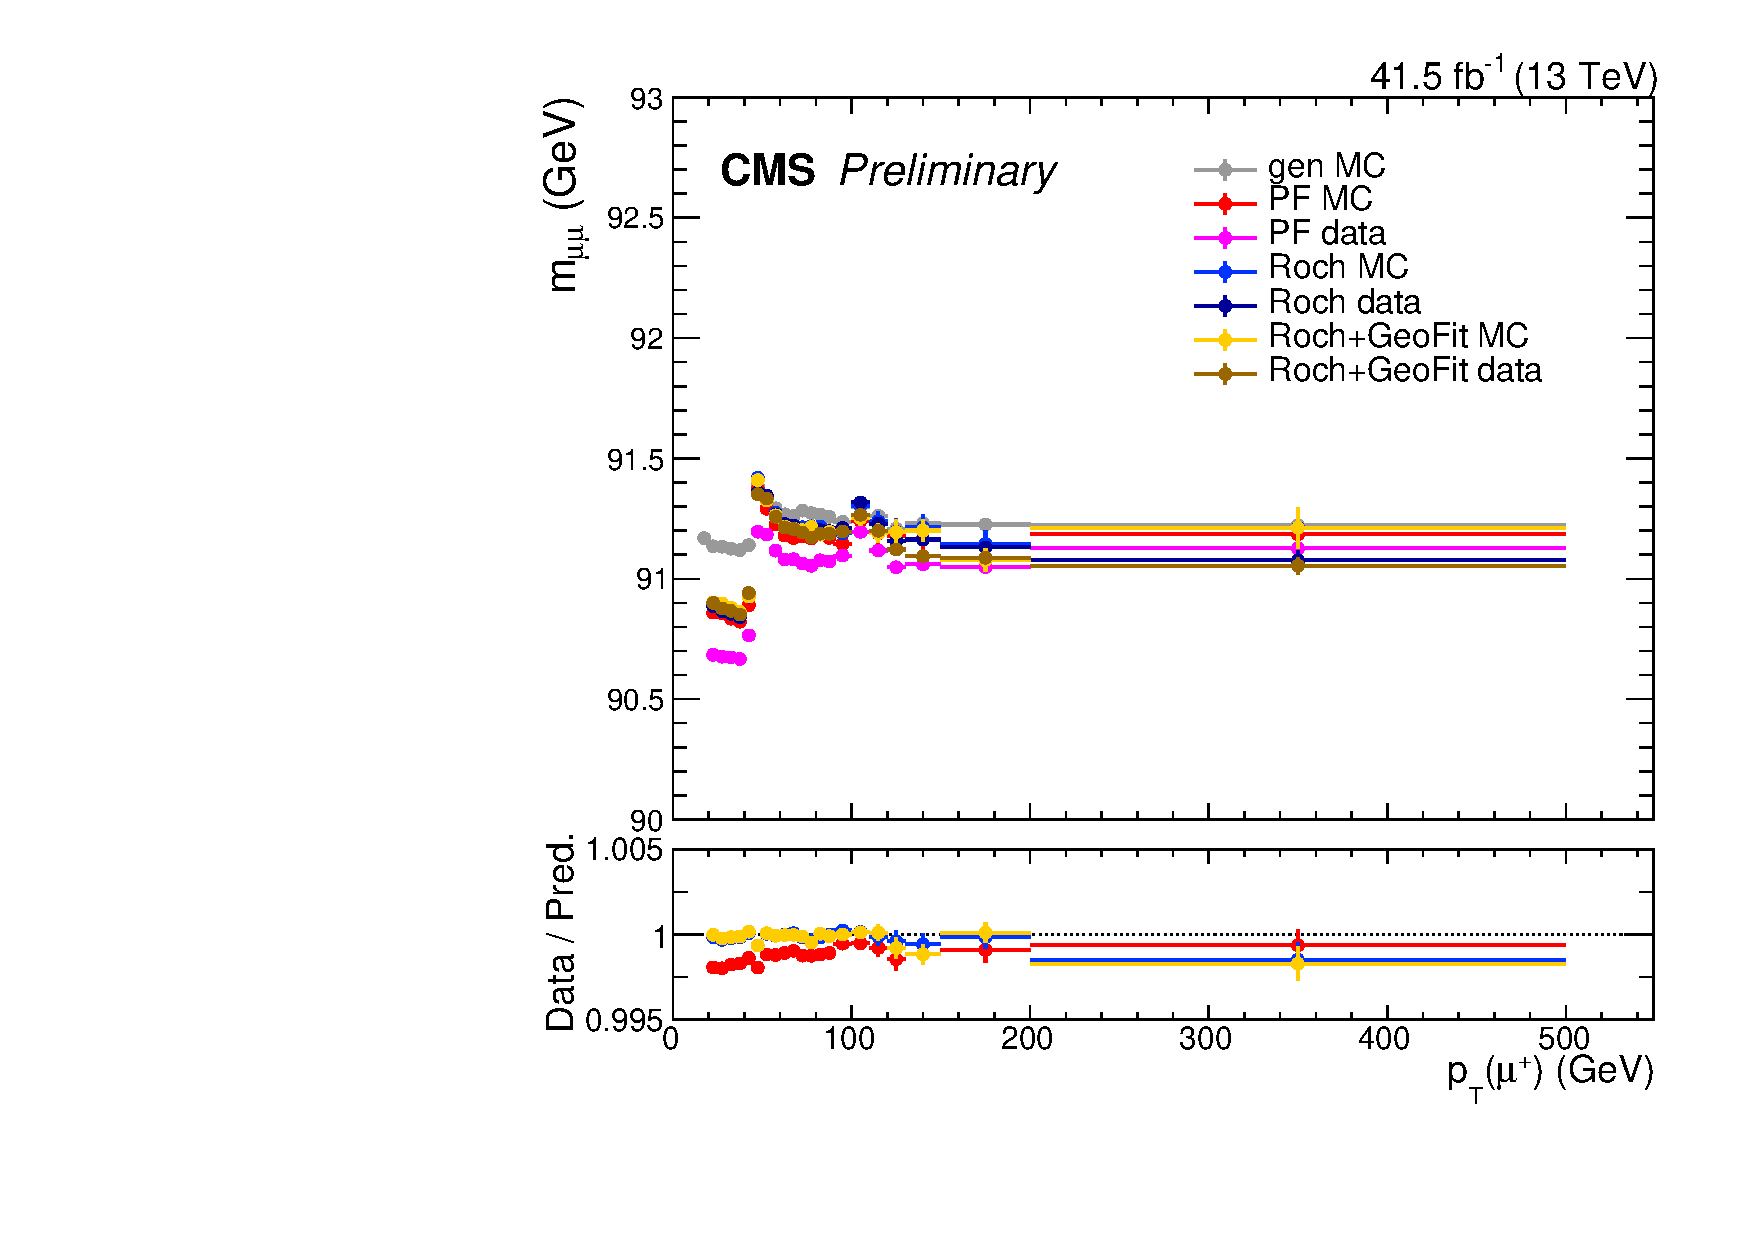
\includegraphics[width=0.32\textwidth]{pics/muon_corr/muon_cal/2017/muP_pt_summary_mean.pdf}
      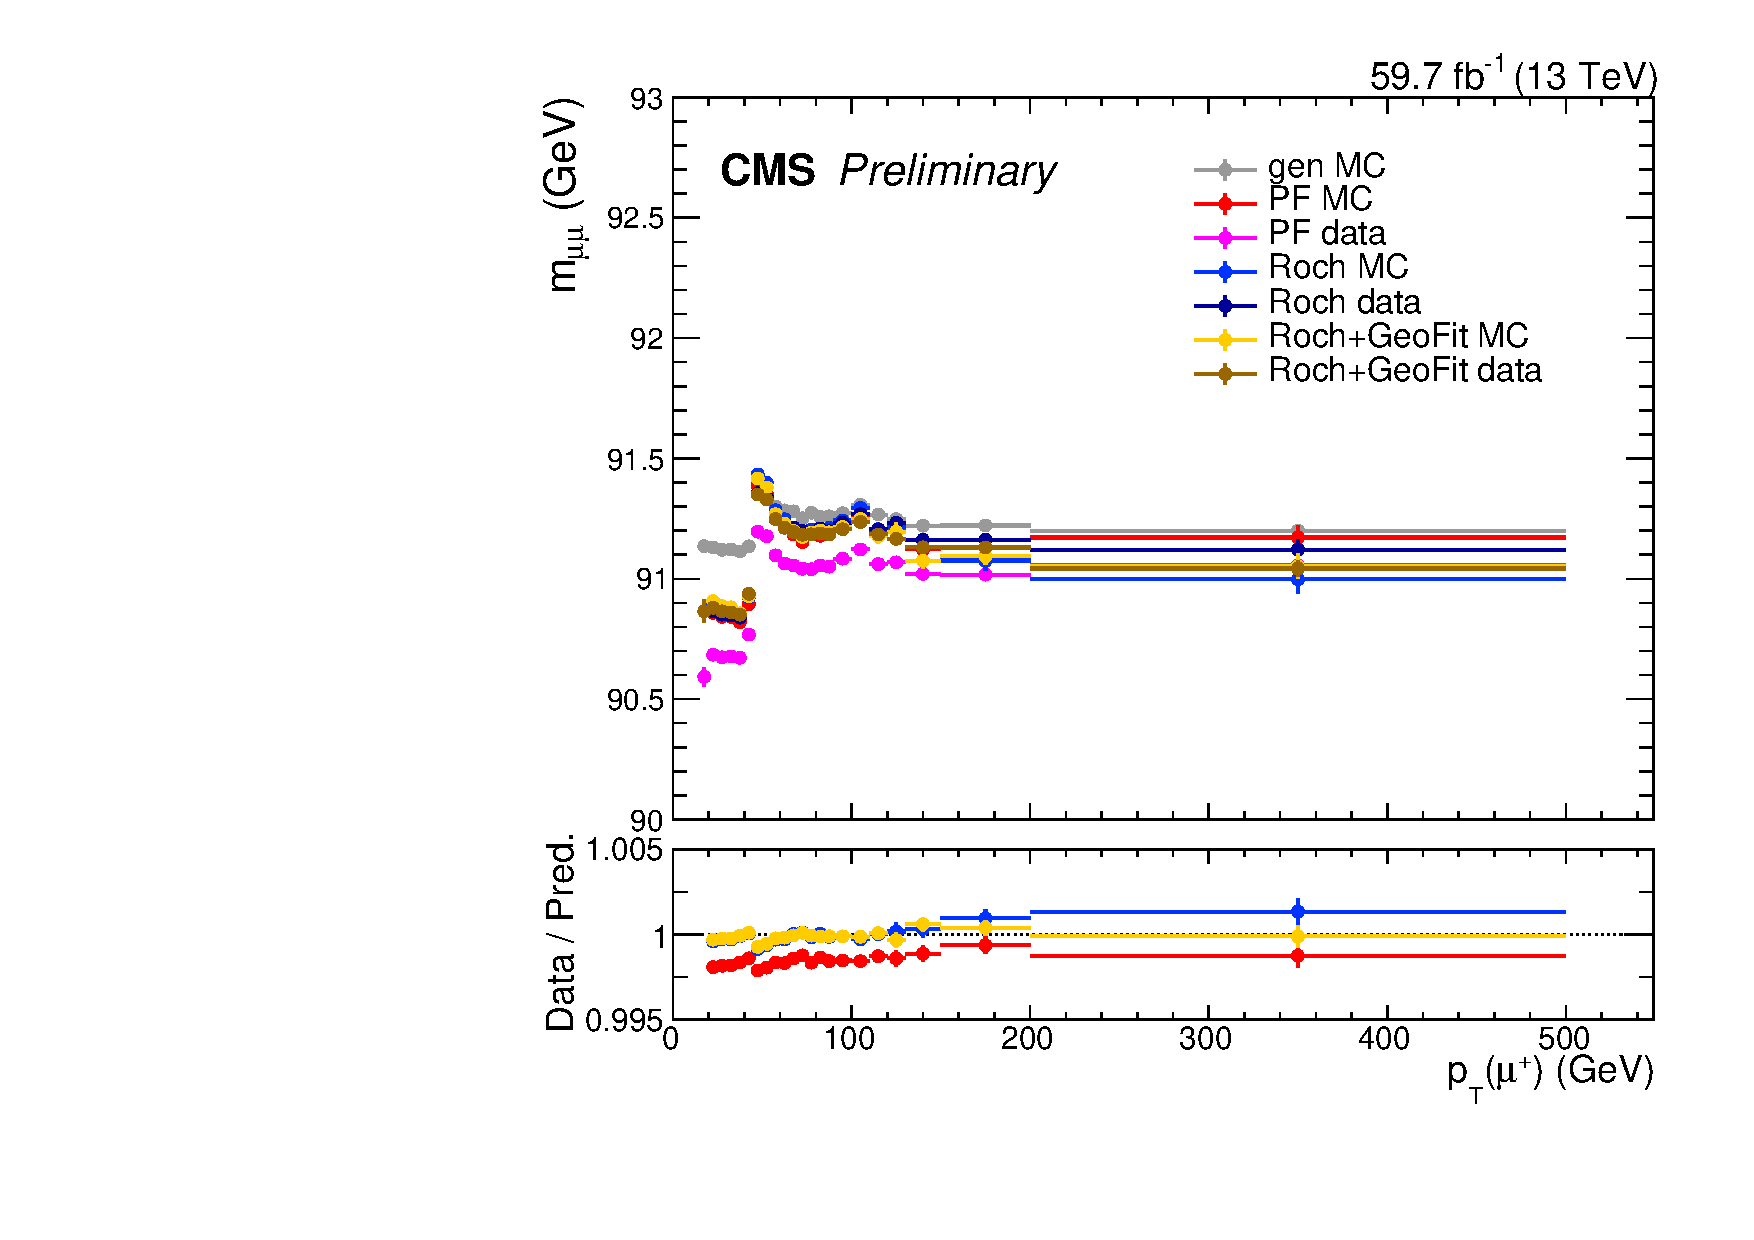
\includegraphics[width=0.32\textwidth]{pics/muon_corr/muon_cal/2018/muP_pt_summary_mean.pdf}
      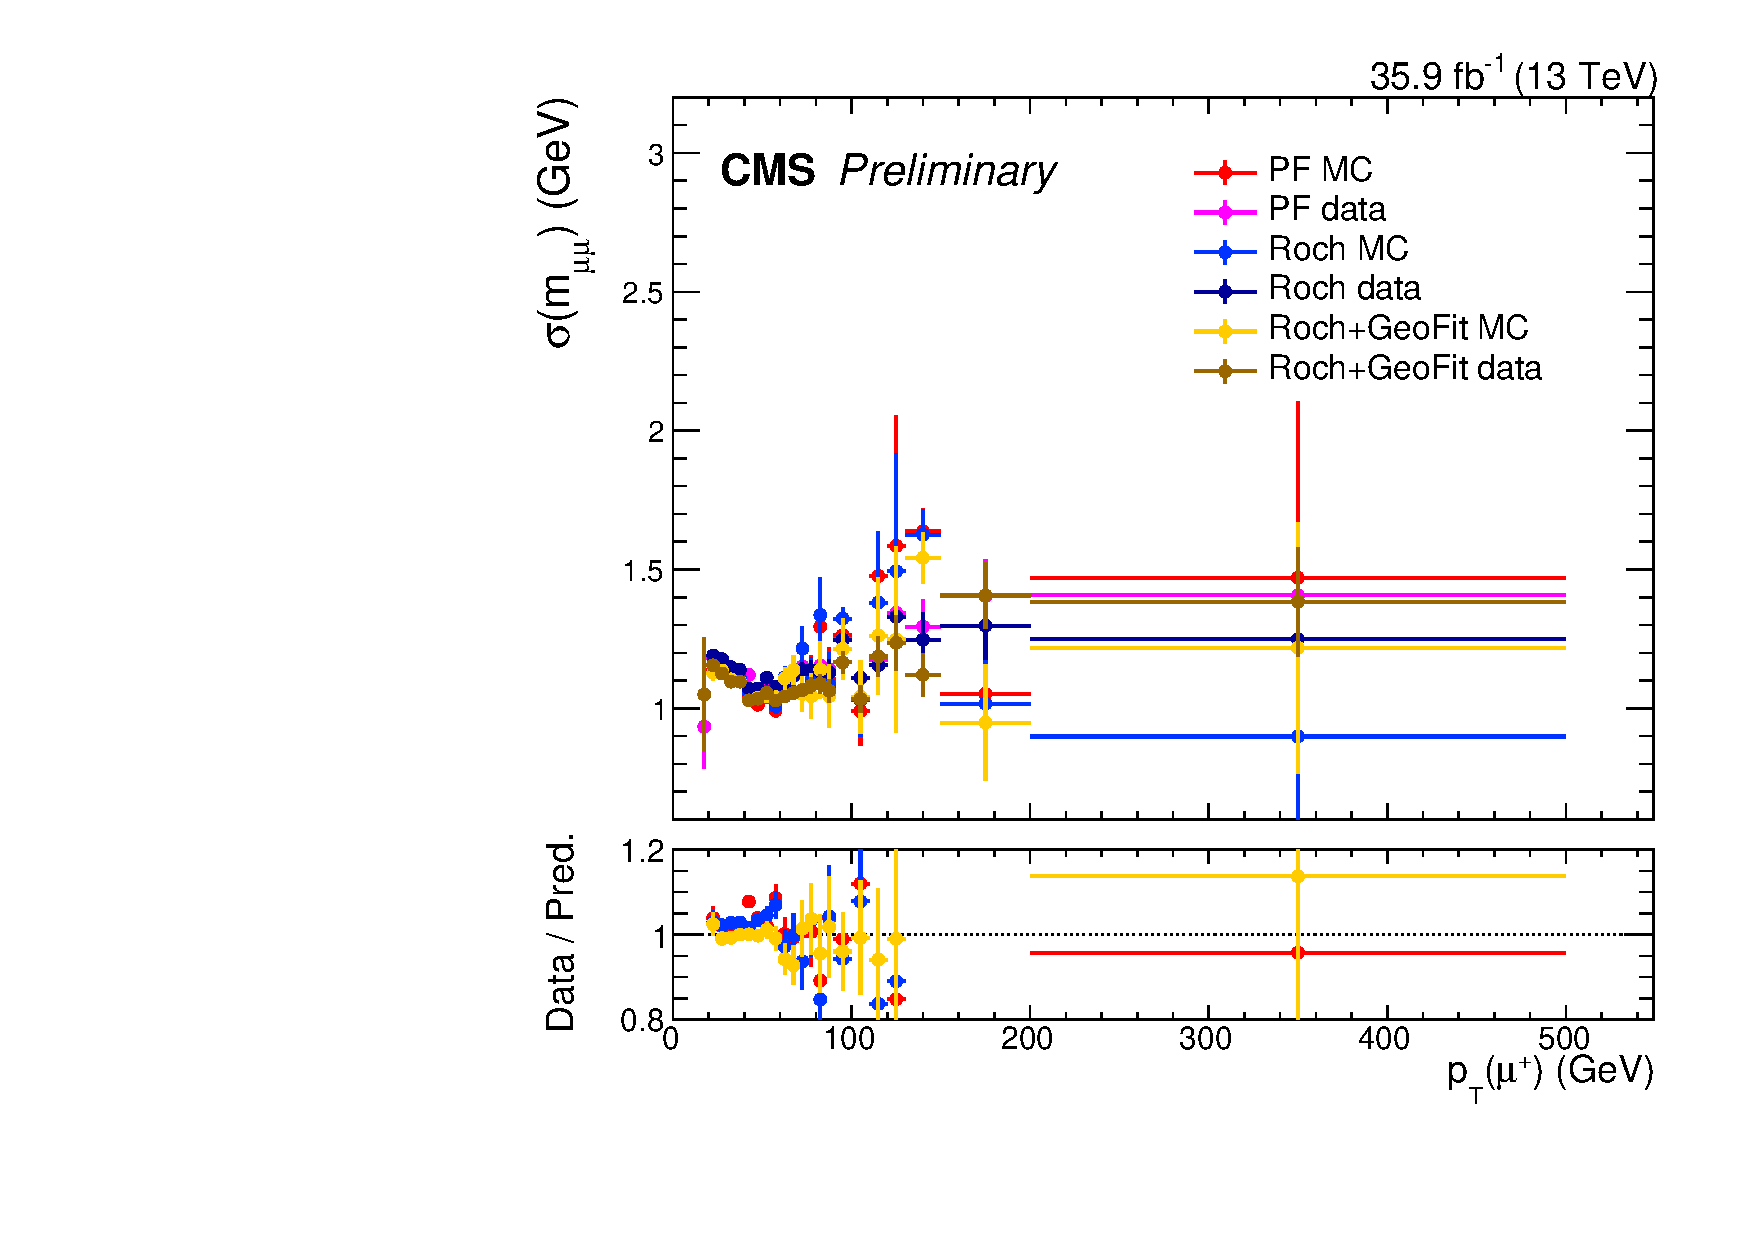
\includegraphics[width=0.32\textwidth]{pics/muon_corr/muon_cal/2016/muP_pt_summary_reso.pdf}
      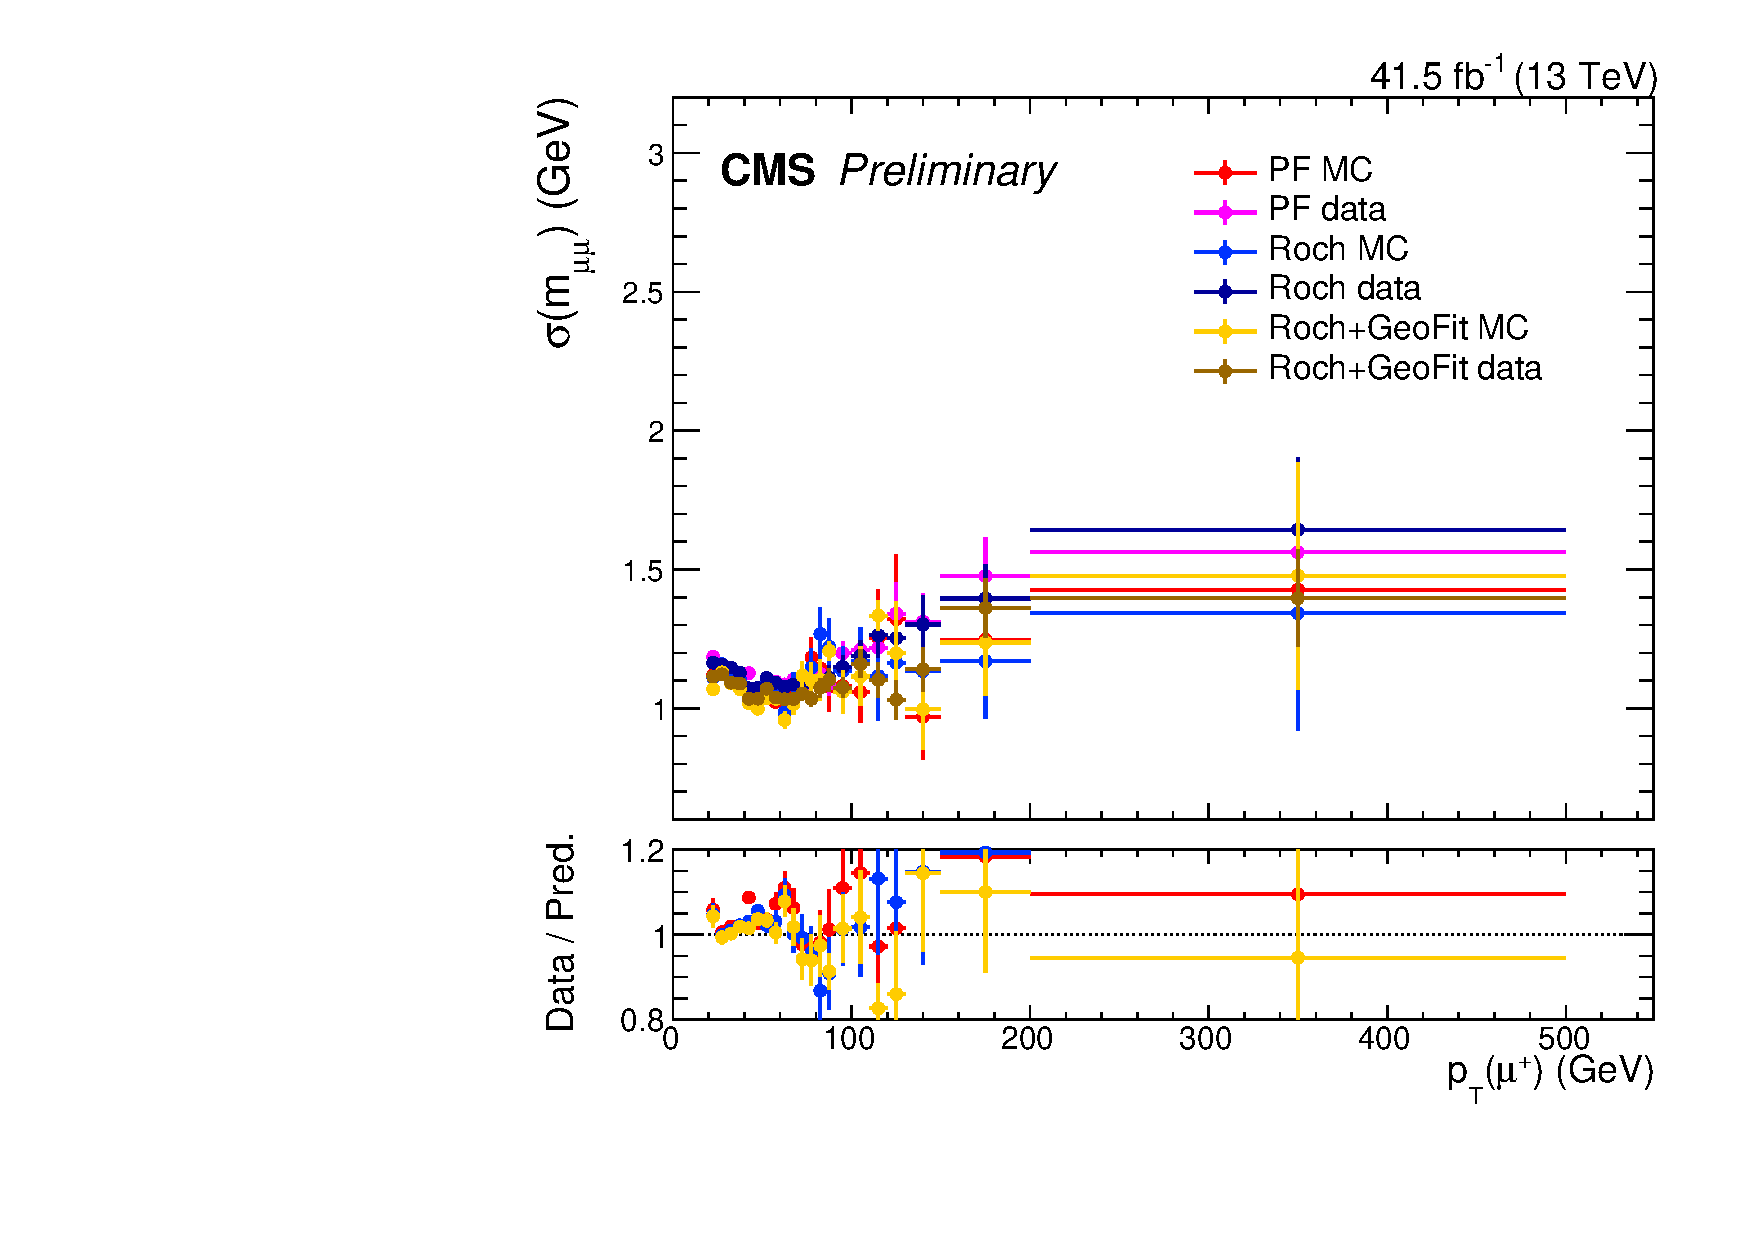
\includegraphics[width=0.32\textwidth]{pics/muon_corr/muon_cal/2017/muP_pt_summary_reso.pdf}
      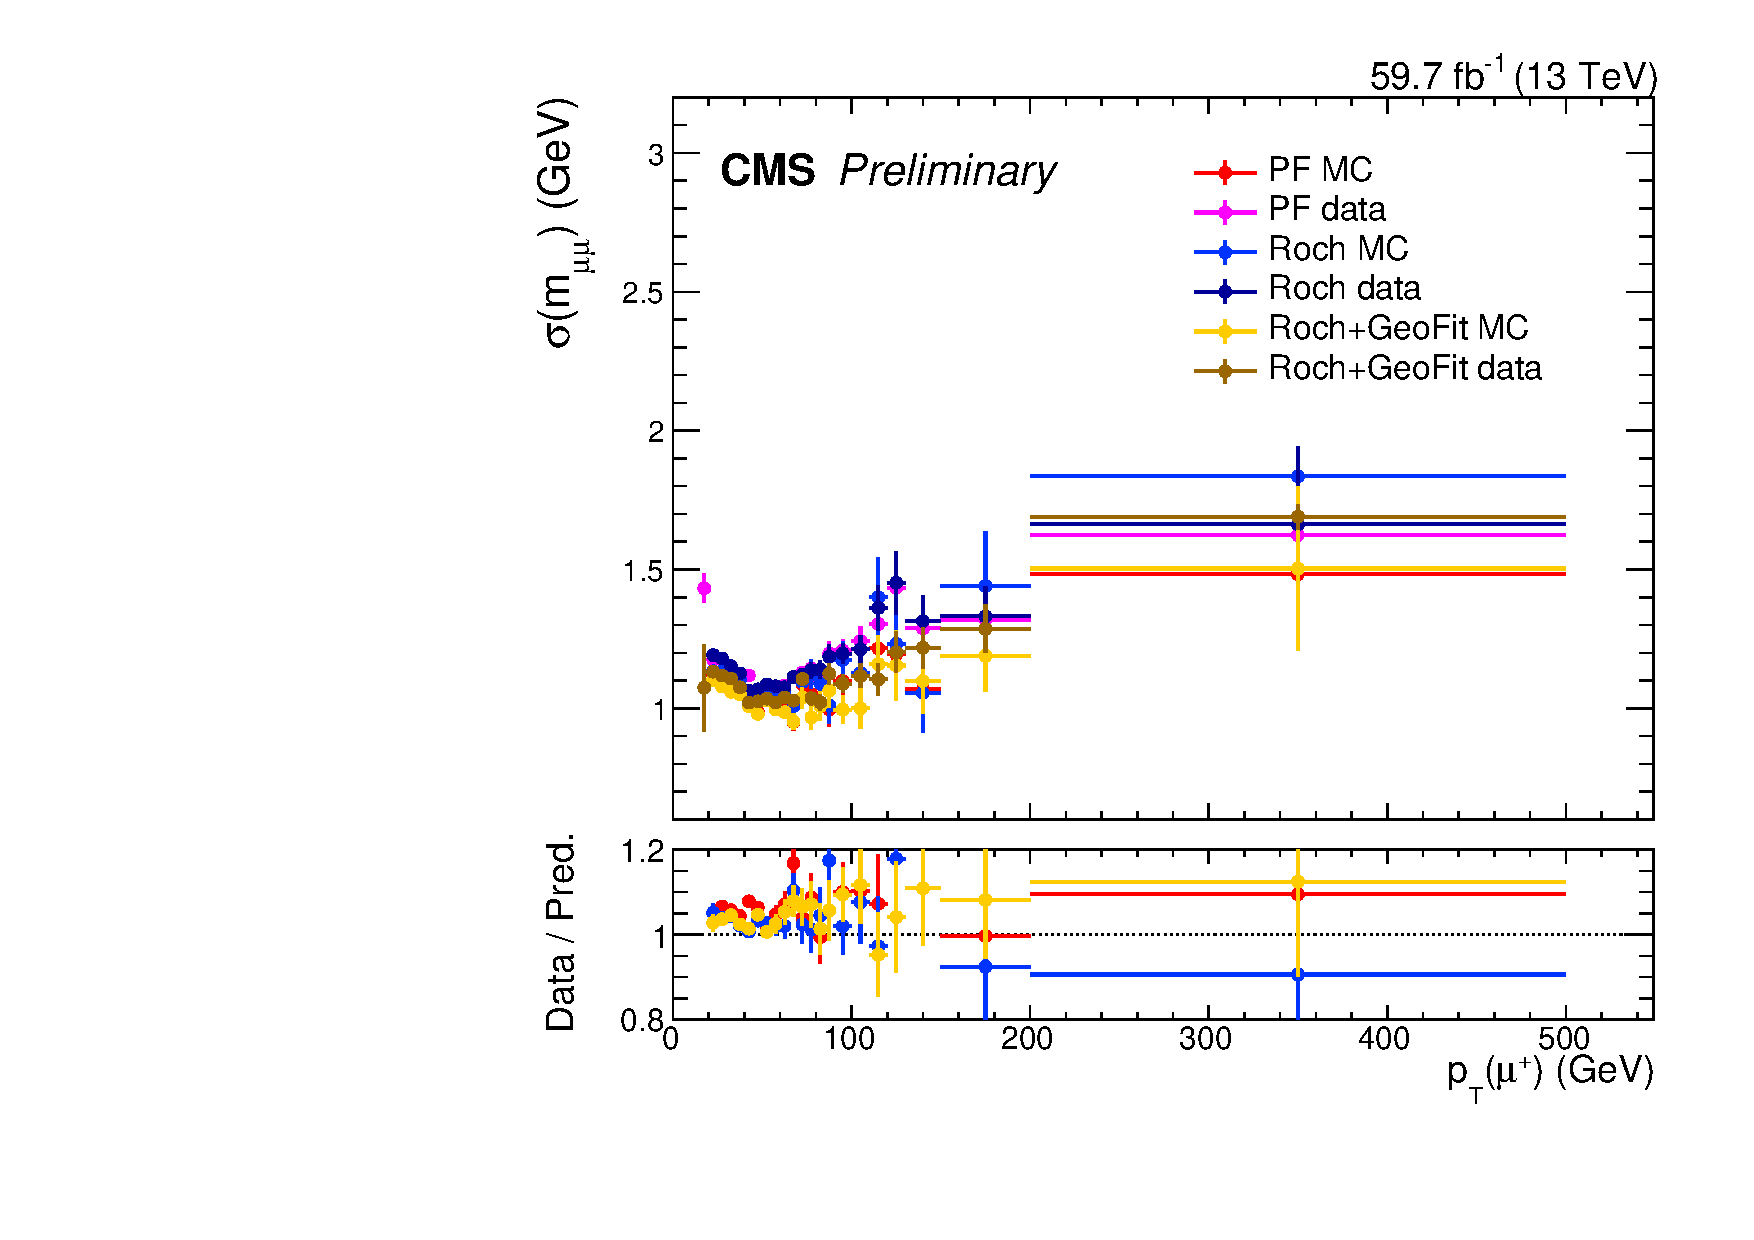
\includegraphics[width=0.32\textwidth]{pics/muon_corr/muon_cal/2018/muP_pt_summary_reso.pdf}
      \caption{Muon calibration plots vs $\pt(\mu^{+})$, for 2016 (left column), 2017 (middle column) and 2018 (right column).
               The top row shows the mean value of the Voigtian fit to the \mmm distribution, 
               while the bottom row shows its experimental resolution.
               The \pt binning sculpts the shape of the \mmm peak, which leads to a jump at the \pt = 45 \GeV in the plots.}
      \label{fig:mucal_muP_pt}
\end{figure*}


\begin{figure*}[!htb]
      \centering
%      \captionsetup{justification=justified}
      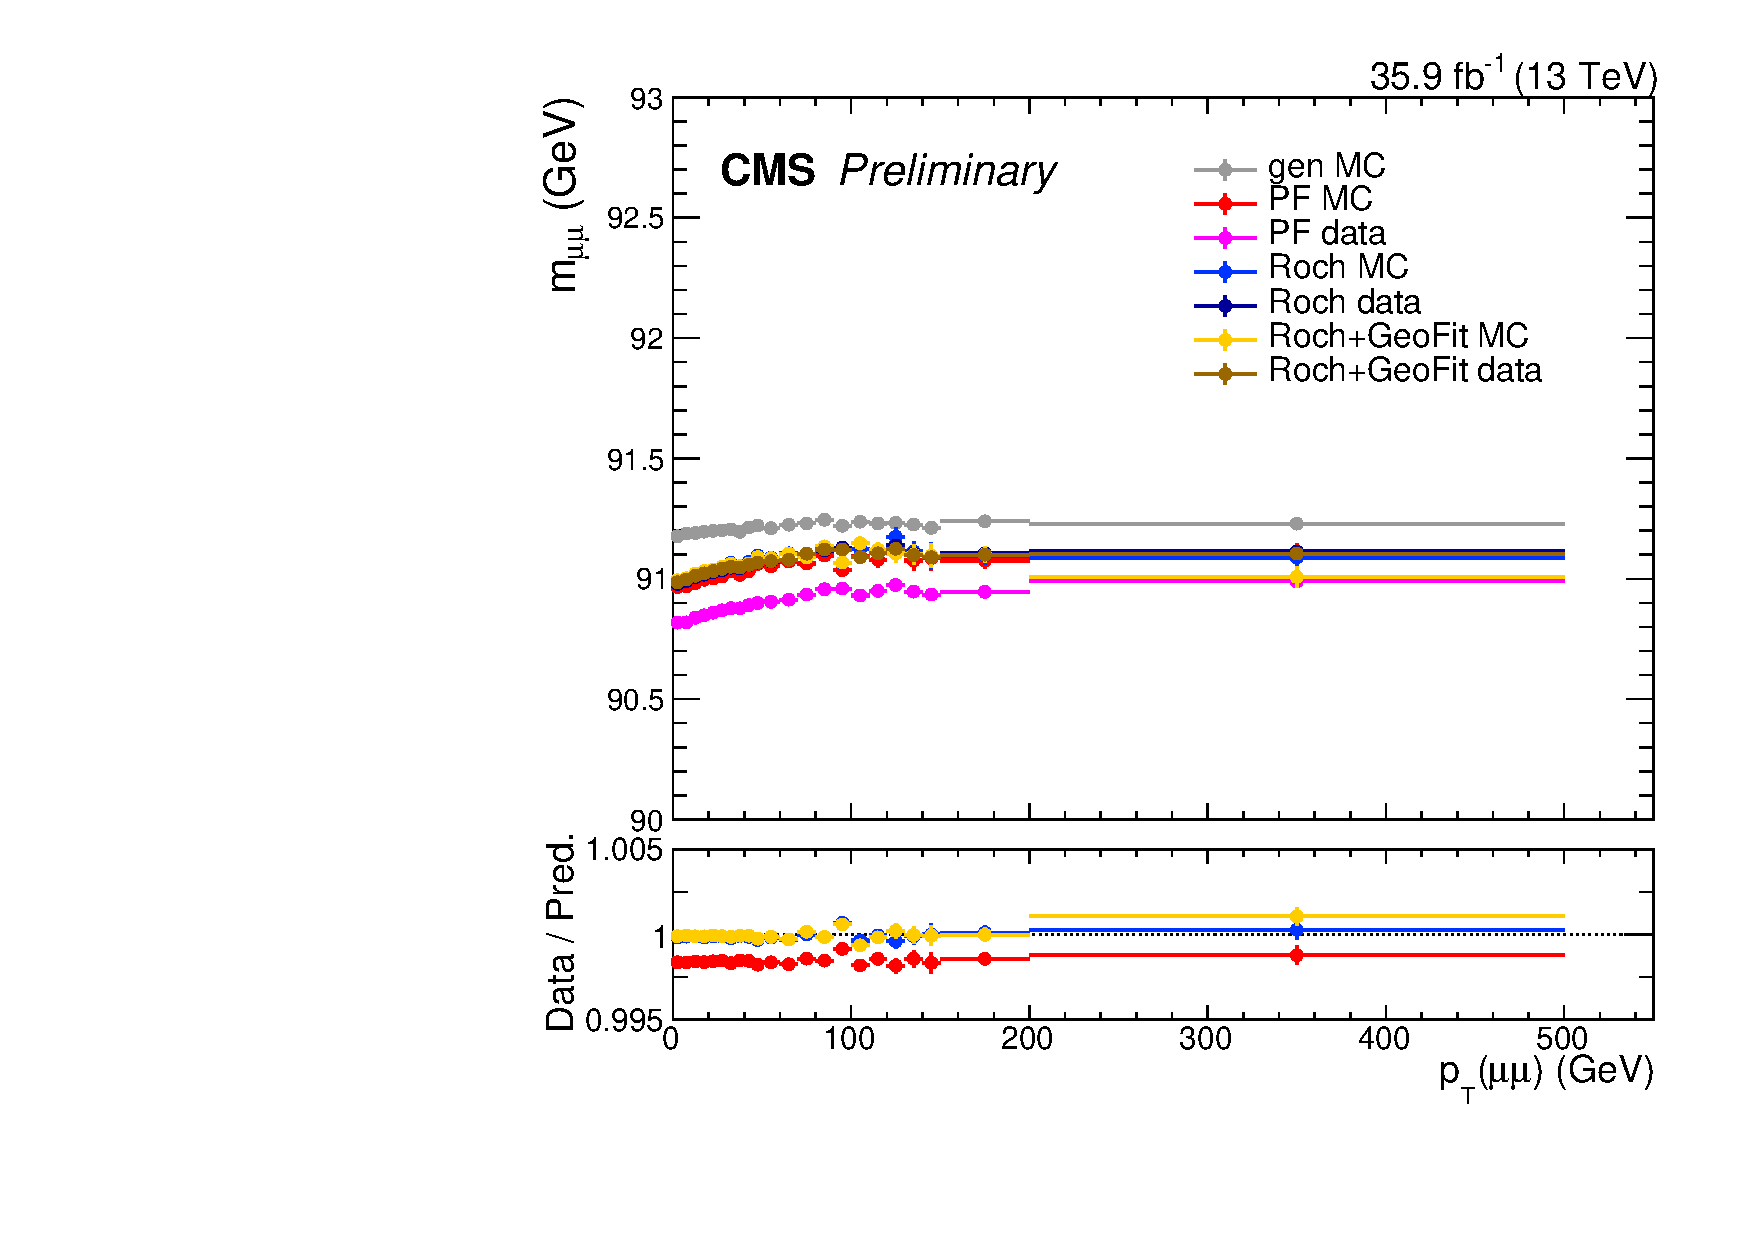
\includegraphics[width=0.32\textwidth]{pics/muon_corr/muon_cal/2016/dimu_pt_summary_mean.pdf}
      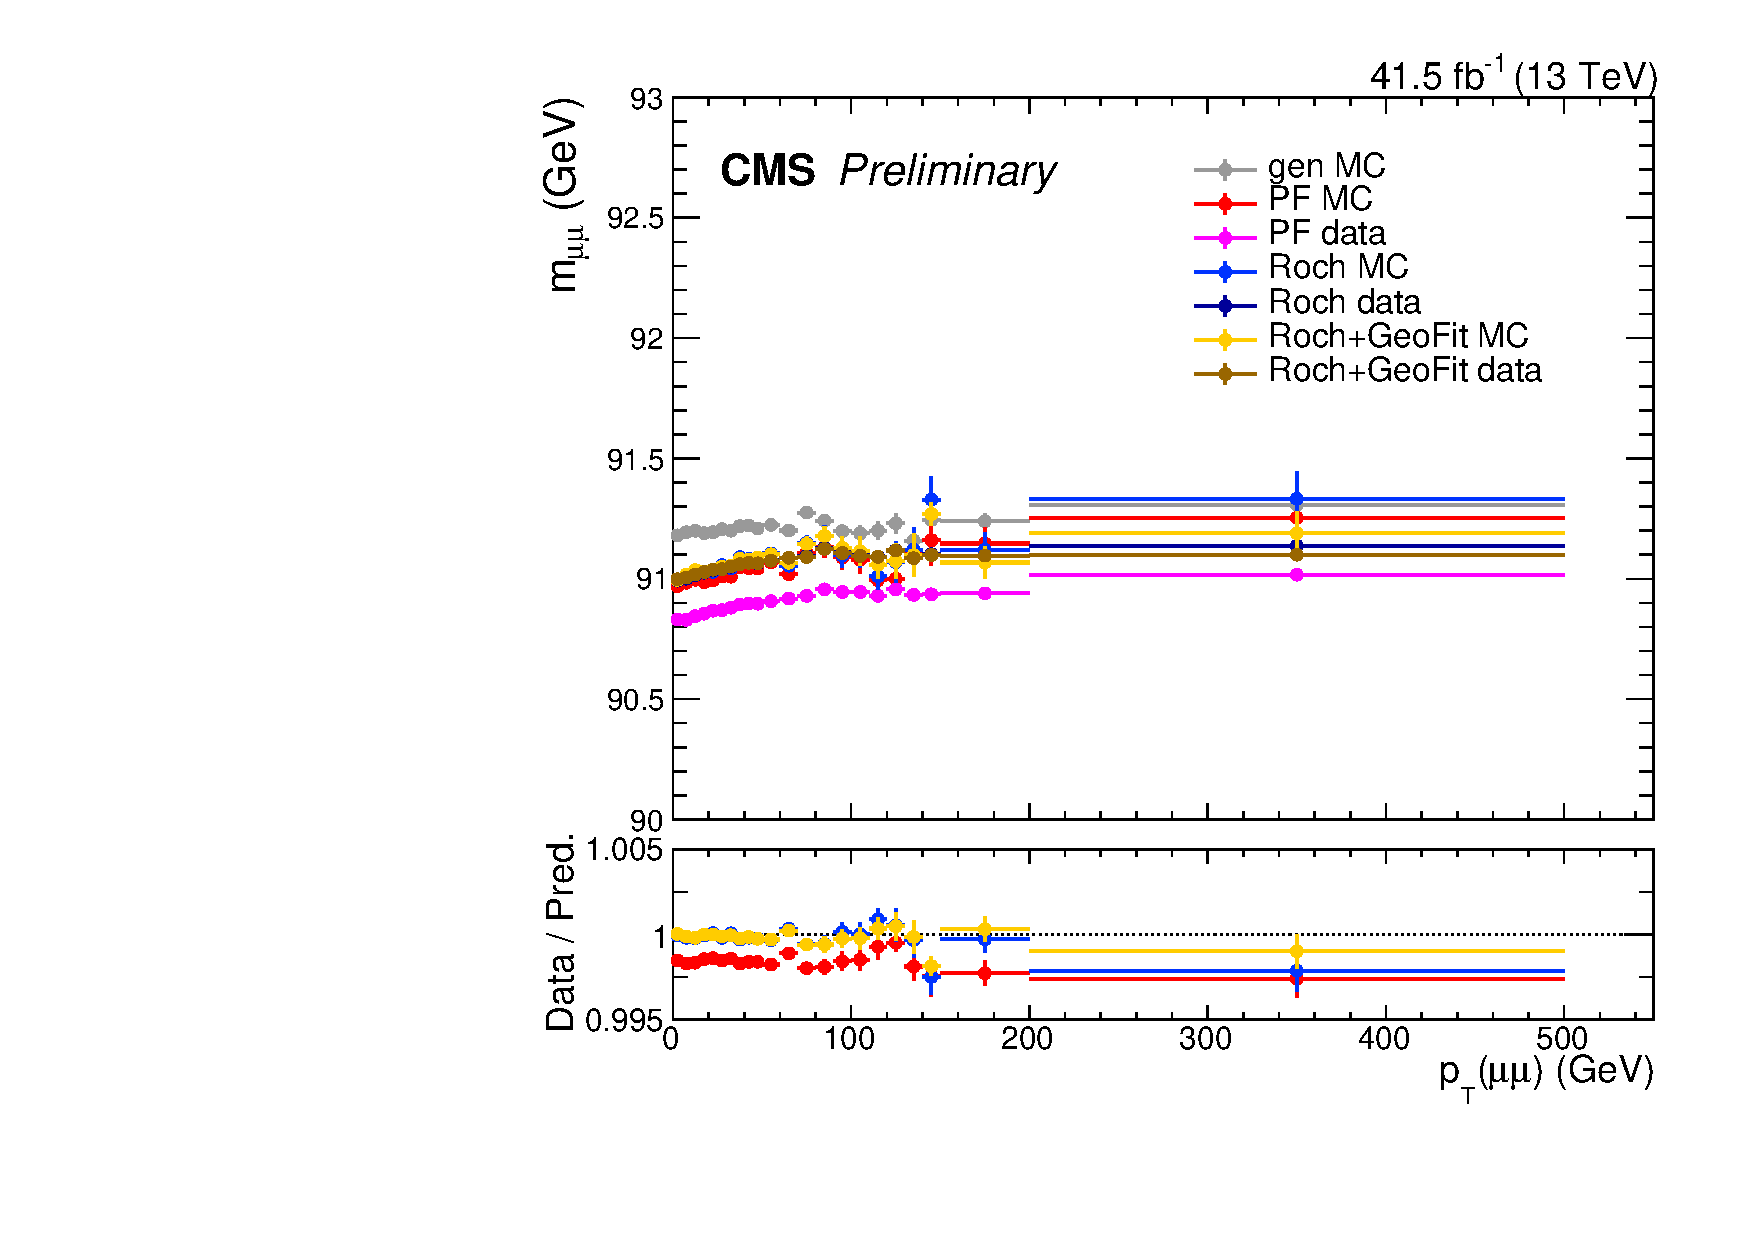
\includegraphics[width=0.32\textwidth]{pics/muon_corr/muon_cal/2017/dimu_pt_summary_mean.pdf}
      \includegraphics[width=0.32\textwidth]{pics/muon_corr/muon_cal/2018/dimu_pt_summary_mean.pdf}
      \includegraphics[width=0.32\textwidth]{pics/muon_corr/muon_cal/2016/dimu_pt_summary_reso.pdf}
      \includegraphics[width=0.32\textwidth]{pics/muon_corr/muon_cal/2017/dimu_pt_summary_reso.pdf}
      \includegraphics[width=0.32\textwidth]{pics/muon_corr/muon_cal/2018/dimu_pt_summary_reso.pdf}
      \caption{Muon calibration plots vs $\pt(\mu\mu)$, for 2016 (left column), 2017 (middle column) and 2018 (right column).
               The top row shows the mean value of the Voigtian fit to the \mmm distribution, 
               while the bottom row shows its experimental resolution.}
      \label{fig:mucal_dimu_pt}
\end{figure*}


\begin{figure*}[!htb]
      \centering
%      \captionsetup{justification=justified}
      \includegraphics[width=0.32\textwidth]{pics/muon_corr/muon_cal/2016/dimu_eta_summary_mean.pdf}
      \includegraphics[width=0.32\textwidth]{pics/muon_corr/muon_cal/2017/dimu_eta_summary_mean.pdf}
      \includegraphics[width=0.32\textwidth]{pics/muon_corr/muon_cal/2018/dimu_eta_summary_mean.pdf}
      \includegraphics[width=0.32\textwidth]{pics/muon_corr/muon_cal/2016/dimu_eta_summary_reso.pdf}
      \includegraphics[width=0.32\textwidth]{pics/muon_corr/muon_cal/2017/dimu_eta_summary_reso.pdf}
      \includegraphics[width=0.32\textwidth]{pics/muon_corr/muon_cal/2018/dimu_eta_summary_reso.pdf}
      \caption{Muon calibration plots vs $\eta(\mu\mu)$, for 2016 (left column), 2017 (middle column) and 2018 (right column).
               The top row shows the mean value of the Voigtian fit to the \mmm distribution, 
               while the bottom row shows its experimental resolution.}
      \label{fig:mucal_dimu_eta}
\end{figure*}


\begin{figure*}[!htb]
      \centering
%      \captionsetup{justification=justified}
      \includegraphics[width=0.32\textwidth]{pics/muon_corr/muon_cal/2016/muP_d0_rebin_summary_mean.pdf}
      \includegraphics[width=0.32\textwidth]{pics/muon_corr/muon_cal/2017/muP_d0_rebin_summary_mean.pdf}
      \includegraphics[width=0.32\textwidth]{pics/muon_corr/muon_cal/2018/muP_d0_rebin_summary_mean.pdf}
      \includegraphics[width=0.32\textwidth]{pics/muon_corr/muon_cal/2016/muP_d0_rebin_summary_reso.pdf}
      \includegraphics[width=0.32\textwidth]{pics/muon_corr/muon_cal/2017/muP_d0_rebin_summary_reso.pdf}
      \includegraphics[width=0.32\textwidth]{pics/muon_corr/muon_cal/2018/muP_d0_rebin_summary_reso.pdf}
      \caption{Muon calibration plots vs $d_0(\mu^{+})$, for 2016 (left column), 2017 (middle column) and 2018 (right column).
               The top row shows the mean value of the Voigtian fit to the \mmm distribution, 
               while the bottom row shows its experimental resolution.}
      \label{fig:mucal_muP_d0}
\end{figure*}


\begin{figure*}[!htb]
      \centering
%      \captionsetup{justification=justified}
      \includegraphics[width=0.32\textwidth]{pics/muon_corr/muon_cal/2016/muN_d0_rebin_summary_mean.pdf}
      \includegraphics[width=0.32\textwidth]{pics/muon_corr/muon_cal/2017/muN_d0_rebin_summary_mean.pdf}
      \includegraphics[width=0.32\textwidth]{pics/muon_corr/muon_cal/2018/muN_d0_rebin_summary_mean.pdf}
      \includegraphics[width=0.32\textwidth]{pics/muon_corr/muon_cal/2016/muN_d0_rebin_summary_reso.pdf}
      \includegraphics[width=0.32\textwidth]{pics/muon_corr/muon_cal/2017/muN_d0_rebin_summary_reso.pdf}
      \includegraphics[width=0.32\textwidth]{pics/muon_corr/muon_cal/2018/muN_d0_rebin_summary_reso.pdf}
      \caption{Muon calibration plots vs $d_0(\mu^{-})$, for 2016 (left column), 2017 (middle column) and 2018 (right column).
               The top row shows the mean value of the Voigtian fit to the \mmm distribution, 
               while the bottom row shows its experimental resolution.}
      \label{fig:mucal_muN_d0}
\end{figure*}